% LaTeX source for ``Think Java2: Data Structures in Java''
% Copyright (C) 2014  Allen B. Downey

% Permission is granted to copy, distribute, transmit and adapt
% this work under a Creative Commons
% Attribution-NonCommercial-ShareAlike 3.0 Unported License:
% http://creativecommons.org/licenses/by-nc-sa/3.0/

% If you are interested in distributing a commercial version of this
% work, please contact Allen B. Downey.

% The original form of this book is LaTeX source code.  Compiling this
% LaTeX source has the effect of generating a device-independent
% representation of the book, which can be converted to other formats
% and printed.

% The LaTeX source for this book is available from http://thinkapjava.com
% and http://code.google.com/p/thinkapjava/source/checkout

% This book was typeset using LaTeX .  The illustrations were
% drawn in xfig.  All of these are free, open-source programs.

%%----------------------------------------------------------------

% How to compile this document:
% If your environment provides latex, makeindex, and dvips,
% the following commands should produce a Postscript version
% of the book.

%        latex book
%        makeindex book
%        latex book
%        dvips -o book.ps book

% You will also need the following (fairly standard) latex
% packages: url, epsfig, makeidx, fancyhdr

% This distribution also includes a Makefile that should
% compile both the Postscript and PDF versions of the book.

%%-----------------------------------------------------------------

\documentclass[12pt]{book}

\usepackage{amsmath}
\usepackage{amsthm}
\usepackage{amssymb}
\usepackage{makeidx}
\usepackage{url}
\usepackage{fancyhdr}
\usepackage{verbatim}
\usepackage{moreverb}
\usepackage{hevea}
\usepackage{upquote}
\usepackage{graphicx}


\newcommand{\thetitle}{Think Java 2: Data Structures in Java}
\newcommand{\theversion}{Version 0.1}

\newif\ifplastex
\plastexfalse

\ifplastex
% PLASTEX ONLY
    \usepackage{localdef}
    \maketitle

\else

% LATEX AND HTML

\newtheoremstyle{exercise}
  {\topsep}     % space above
  {\topsep}     % space below
  {}            % body font
  {}            % indent amount
  {\bfseries}   % head font
  {.}           % punctuation
  {5pt}         % head space
  {}            % custom head
\theoremstyle{exercise}
\newtheorem{exercise}{Exercise}[chapter]

\title{\thetitle}

\author{Allen B. Downey}

% these styles get translated in CSS for the HTML version
\newstyle{a:link}{color:black;}
\newstyle{pre}{color:darkgreen;font-size:110\%;}
\newstyle{tt}{color:darkgreen;font-size:110\%;}
\newstyle{p+p}{margin-top:1em;margin-bottom:1em}
\newstyle{img}{border:0px}

% change the arrows
\setlinkstext
  {\imgsrc[ALT="Previous"]{back.png}}
  {\imgsrc[ALT="Up"]{up.png}}
  {\imgsrc[ALT="Next"]{next.png}}

\makeindex

% define styles for syntax highlighting in code listings
\usepackage[usenames,dvipsnames]{color}
\usepackage{listings}
\lstset{
    language=java,
    basicstyle=\ttfamily,
    commentstyle=\color{Green},
    keywordstyle=\color{blue},
    stringstyle=\color{Orange},
    columns=fullflexible,
    keepspaces=true,
    showstringspaces=false,
    aboveskip=4pt,
    belowskip=-4pt
}

% enable pdf hyperlinks, table of contents, and document properties
\usepackage[pdftex]{hyperref}
\makeatletter
\hypersetup{%
  pdftitle={\@title},
  pdfauthor={\@author},
  pdfsubject={Version \theversion},
  pdfkeywords={},
  bookmarksopen=false,
  colorlinks=true,
  citecolor=black,
  filecolor=black,
  linkcolor=black,
  urlcolor=blue
}
\makeatother

\begin{document}

\frontmatter

% title page for the HTML version

\begin{htmlonly}

% TITLE PAGE FOR HTML VERSION

{\Large Think Java 2}

{\large Allen B. Downey}

Version \theversion

\setcounter{chapter}{-1}

\end{htmlonly}

% BEGINNING OF LATEXONLY

\input{latexonly}

\begin{latexonly}

%-half title--------------------------------------------------

%\thispagestyle{empty}
%
%\begin{flushright}
%\vspace*{2.5in}
%
%{\huge Think Java}
%
%\vspace{1in}
%
%{\LARGE How to Think Like a Computer Scientist}
%
%\vfill
%
%\end{flushright}

%--verso------------------------------------------------------

%%\clearemptydoublepage
%\cleardoublepage

%--title page--------------------------------------------------
\pagebreak
\thispagestyle{empty}

\begin{flushright}
\vspace*{2.5in}

{\huge Think Java 2}

\vspace{0.25in}

{\LARGE Data Structures in Java}

\vspace{1in}

{\Large
Allen B. Downey
}


\vspace{1in}

{\Large \theversion}

\vfill

\end{flushright}


%--copyright--------------------------------------------------
\pagebreak
\thispagestyle{empty}

Copyright \copyright ~2014 Allen Downey.

\vspace{0.25in}

Permission is granted to copy, distribute, transmit and adapt
this work under a Creative Commons
Attribution-NonCommercial-ShareAlike 3.0 Unported License:
\url{http://creativecommons.org/licenses/by-nc-sa/3.0/}

If you are interested in distributing a commercial version of this
work, please contact Allen B. Downey.

The original form of this book is \LaTeX\ source code.  Compiling this
\LaTeX\ source has the effect of generating a device-independent
representation of the book, which can be converted to other formats
and printed.

The \LaTeX\ source for this book is available from:
\url{http://thinkapjava.com}

This book was typeset using \LaTeX .  The illustrations were
drawn in xfig.  All of these are free, open-source programs.

\vspace{0.25in}


%-----------------------------------------------------------------

\end{latexonly}

\fi
% END OF THE PART WE SKIP FOR PLASTEX

\chapter{Preface}



\section*{Contributors List}

When I started writing free books, it didn't occur to me to keep
a contributors list.  When Jeff Elkner suggested it, it seemed so
obvious that I am embarassed by the omission.  This list starts
with the 4th Edition, so it omits many people who contributed
suggestions and corrections to earlier versions.

If you have additional comments, please send them to: \\
\href{mailto:feedback@greenteapress.com}{feedback@greenteapress.com}

\begin{itemize}

\item Ellen Hildreth used a previous version of this book to teach
  Data Structures at Wellesley College, and she gave me a whole stack
  of corrections, along with some great suggestions.


\end{itemize}

% endcontrib

% table of contents

\setcounter{tocdepth}{1}
\tableofcontents

% main matter
\mainmatter

\chapter{Linked lists}
\label{list}
\index{list}

\section{References in objects}
\index{reference}
\index{embedded reference}
\index{reference!embedded}
\index{node}
\index{cargo}

In the last chapter we saw that the instance variables of an
object can be arrays, and I mentioned that they can be objects,
too.

One of the more interesting possibilities is that an object
can contain a reference to another object of the same type.
There is a common data structure, the {\bf list}, that takes advantage
of this feature.

Lists are made up of {\bf nodes}, where each node contains a
reference to the next node in the list.  In addition, each node
usually contains a unit of data called the {\bf cargo}.  In our
first example, the cargo will be a single integer, but later we
will write a {\bf generic} list that can contain objects
of any type.

\index{generic data structure}
\index{data structure!generic}

\section{The {\tt Node} class}
\index{Node class}
\index{class!Node}

As usual when we write a new class, we'll start with the instance
variables, one or two constructors and {\tt toString} so that we
can test the basic mechanism of creating and displaying the new
type.

\begin{verbatim}
public class Node {
    int cargo;
    Node next;

    public Node () {
        cargo = 0;
        next = null;
    }

    public Node (int cargo, Node next) {
        this.cargo = cargo;
        this.next = next;
    }

    public String toString () {
        return cargo + "";
    }
}
\end{verbatim}
%
The declarations of the instance variables follow naturally
from the specification, and the rest follows mechanically from
the instance variables.  The expression {\tt cargo + ""} is
an awkward but concise way to convert an integer to a String.

To test the implementation so far, we would put something like
this in {\tt main}:

\begin{verbatim}
    Node node = new Node (1, null);
    System.out.println (node);
\end{verbatim}
%
The result is simply

\begin{verbatim}
1
\end{verbatim}
%
To make it interesting, we need a list with more than
one node!

\begin{verbatim}
    Node node1 = new Node (1, null);
    Node node2 = new Node (2, null);
    Node node3 = new Node (3, null);
\end{verbatim}
%
This code creates three nodes, but we don't have a list yet
because the nodes are not {\bf linked}.  The state diagram
looks like this:


\includegraphics{figs/list1.pdf}


To link up the nodes, we have to make the first node refer to the
second and the second node refer to the third.

\begin{verbatim}
    node1.next = node2;
    node2.next = node3;
    node3.next = null;
\end{verbatim}
%
The reference of the third node is {\tt null}, which indicates that
it is the end of the list.  Now the state diagram looks like:


\includegraphics{figs/list2.pdf}


Now we know how to create nodes and link them into lists.  What
might be less clear at this point is why.

\section{Lists as collections}
\index{collection}

The thing that makes lists useful is that they are a way of assembling
multiple objects into a single entity, sometimes called a collection.
In the example, the first node of the list serves as a reference to
the entire list.

\index{list!printing}
\index{list!as parameter}

If we want to pass the list as a parameter, all we have to pass is a
reference to the first node.  For example, the method {\tt printList}
takes a single node as an argument.  Starting with the head of the
list, it prints each node until it gets to the end (indicated by the
{\tt null} reference).

\begin{verbatim}
    public static void printList (Node list) {
        Node node = list;

        while (node != null) {
            System.out.print (node);
            node = node.next;
        }
        System.out.println ();
    }
\end{verbatim}
%
To invoke this method we just have to pass a reference to the
first node:

\begin{verbatim}
        printList (node1);
\end{verbatim}
%
Inside {\tt printList} we have a reference to the first node
of the list, but there is no variable that refers to the other
nodes.  We have to use the {\tt next} value from each node
to get to the next node.

This diagram shows the value of {\tt list} and the values that
{\tt node} takes on:

\includegraphics{figs/list3.pdf}

This way of moving through a list is called a {\bf traversal},
just like the similar pattern of moving through the elements of
an array.  It is common to use a loop variable like {\tt node}
to refer to each of the nodes in the list in succession.

\index{loop variable}
\index{list!traversal}
\index{traverse}

The output of this method is

\begin{verbatim}
123
\end{verbatim}
%
By convention, lists are printed in parentheses with commas
between the elements, as in {\tt (1, 2, 3)}.  As an exercise, modify
{\tt printList} so that it generates output in this format.

As another exercise, rewrite {\tt printList} using a {\tt for} loop
instead of a {\tt while} loop.

\section{Lists and recursion}
\index{list!traverse recursively}
\index{traverse}

Recursion and lists go together like fava beans and a nice
Chianti.  For example, here is a recursive algorithm for printing
a list backwards:

\index{fava beans}
\index{Chianti}

\begin{enumerate}

\item Separate the list into two pieces: the first node (called
the head) and the rest (called the tail).

\item Print the tail backwards.

\item Print the head.

\end{enumerate}

Of course, Step 2, the recursive call, assumes that we have a way of
printing a list backwards.  But {\em if} we assume that the recursive
call works---the leap of faith---then we can convince ourselves that
this algorithm works.

\index{leap of faith}
\index{list!printing backwards}

All we need is a base case, and a way of proving that for
any list we will eventually get to the base case.  A natural
choice for the base case is a list with a single element, but
an even better choice is the empty list, represented by null.

\begin{verbatim}
    public static void printBackward (Node list) {
        if (list == null) return;

        Node head = list;
        Node tail = list.next;

        printBackward (tail);
        System.out.print (head);
    }    
\end{verbatim}
%
The first line handles the base case by doing nothing.  The
next two lines split the list into {\tt head} and {\tt tail}.
The last two lines print the list.

We invoke this method exactly as we invoked {\tt printList}:

\begin{verbatim}
        printBackward (node1);
\end{verbatim}
%
The result is a backwards list.

Can we prove that this method will always terminate?   In other
words, will it always reach the base case?  In fact, the answer
is no.  There are some lists that will make this method crash.


\section{Infinite lists}
\index{infinite list}
\index{list!infinite}
\index{loop!in list}
\index{list!loop}

There is nothing to prevent a node from referring back to
an earlier node in the list, including itself.  For example,
this figure shows a list with two nodes, one of which refers
to itself.

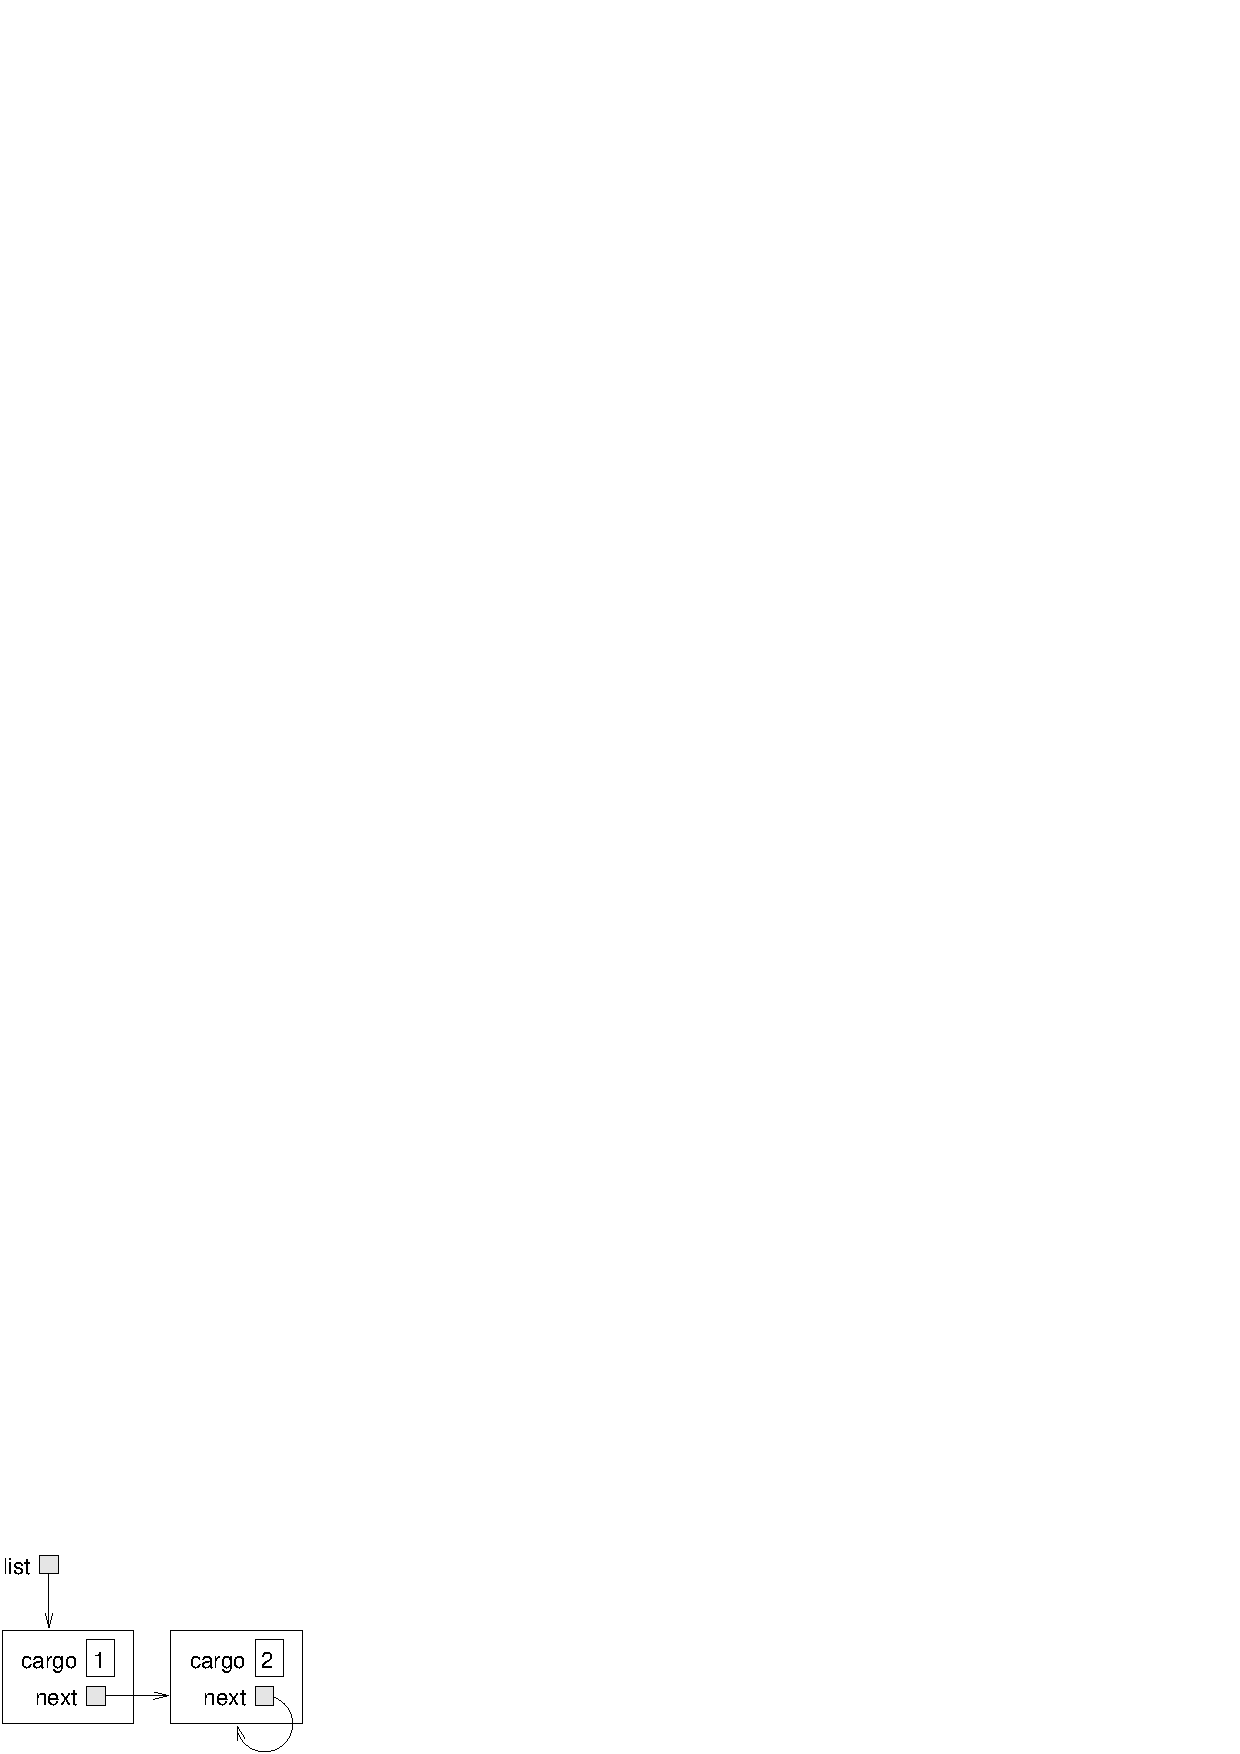
\includegraphics{figs/list4.pdf}

If we invoke {\tt printList} on this list, it will loop forever.
If we invoke {\tt printBackward} it will recurse infinitely.
This sort of behavior makes infinite lists difficult to work
with.

Nevertheless, they are occasionally useful.  For example, we
might represent a number as a list of digits and use an infinite
list to represent a repeating fraction.

Regardless, it is problematic that we cannot prove that {\tt printList}
and {\tt printBackward} terminate.  The best we can do is the
hypothetical statement, ``If the list contains no loops, then these
methods will terminate.''  This sort of claim is called a {\bf
precondition}.  It imposes a constraint on one of the parameters and
describes the behavior of the method if the constraint is satisfied.
We will see more examples soon.

\index{precondition}

\section{The fundamental ambiguity theorem}
\index{ambiguity!fundamental theorem}
\index{theorem!fundamental ambiguity}

There is a part of {\tt printBackward} that might have raised
an eyebrow:

\begin{verbatim}
        Node head = list;
        Node tail = list.next;
\end{verbatim}
%
After the first assignment, {\tt head} and {\tt list} have the same
type and the same value.  So why did I create a new variable?

The reason is that the two variables play different roles.  We think
of {\tt head} as a reference to a single node, and we think of
{\tt list} as a reference to the first node of a list.  These
``roles'' are not part of the program; they are in the mind of the
programmer.

\index{variable!roles}
\index{role!variable}

The second assignment creates a new reference to the second node
in the list, but in this case we think of it as a list.
So, even though {\tt head} and {\tt tail} have the same
type, they play different roles.

This ambiguity is useful, but it can make programs with lists
difficult to read.  I often use variable names like {\tt node}
and {\tt list} to document how I intend to use a variable, and
sometimes I create additional variables to disambiguate.

I could have written {\tt printBackward} without {\tt head}
and {\tt tail}, but I think it makes it harder to understand:

\begin{verbatim}
    public static void printBackward (Node list) {
        if (list == null) return;

        printBackward (list.next);
        System.out.print (list);
    }    

\end{verbatim}
%
Looking at the two function calls, we have to remember that
{\tt printBackward} treats its argument as a list and {\tt print}
treats its argument as a single object.

Always keep in mind the {\bf fundamental ambiguity theorem}:

\begin{quote}
A variable that refers to a node
might treat the node as a single object or as the first
in a list of nodes.
\end{quote}


\section{Object methods for nodes}
\index{method!object}
\index{node!object method}

You might have wondered why {\tt printList} and {\tt printBackward}
are class methods.  I have made the claim that anything that can
be done with class methods can also be done with object methods;
it's just a question of which form is cleaner.

In this case there is a legitimate reason to choose
class methods.  It is legal to send {\tt null}
as an argument to a class method, but it is not legal to invoke
an object method on a null object.

\begin{verbatim}
	Node node = null;
	printList (node);       // legal
	node.printList ();      // NullPointerException
\end{verbatim}
%
This limitation makes it awkward to write list-manipulating
code in a clean, object-oriented style.  A little later we
will see a way to get around this, though.


\section{Modifying lists}
\index{list!modifying}
\index{modifying lists}

Obviously one way to modify a list is to change the cargo of
one of the nodes, but the more interesting operations are the
ones that add, remove, or reorder the nodes.

As an example, we'll write a method that removes the second
node in the list and returns a reference to the removed node.

\begin{verbatim}
    public static Node removeSecond (Node list) {
        Node first = list;
        Node second = list.next;

        // make the first node refer to the third
        first.next = second.next;

        // separate the second node from the rest of the list
        second.next = null;
        return second;
    }
\end{verbatim}
%
Again, I am using temporary variables to make the code more
readable.  Here is how to use this method.

\begin{verbatim}
        printList (node1);
        Node removed = removeSecond (node1);
        printList (removed);
        printList (node1);
\end{verbatim}
%
The output is

\begin{verbatim}
(1, 2, 3)           the original list
(2)                 the removed node
(1, 3)              the modified list
\end{verbatim}
%
Here is a state diagram showing the effect of this operation.

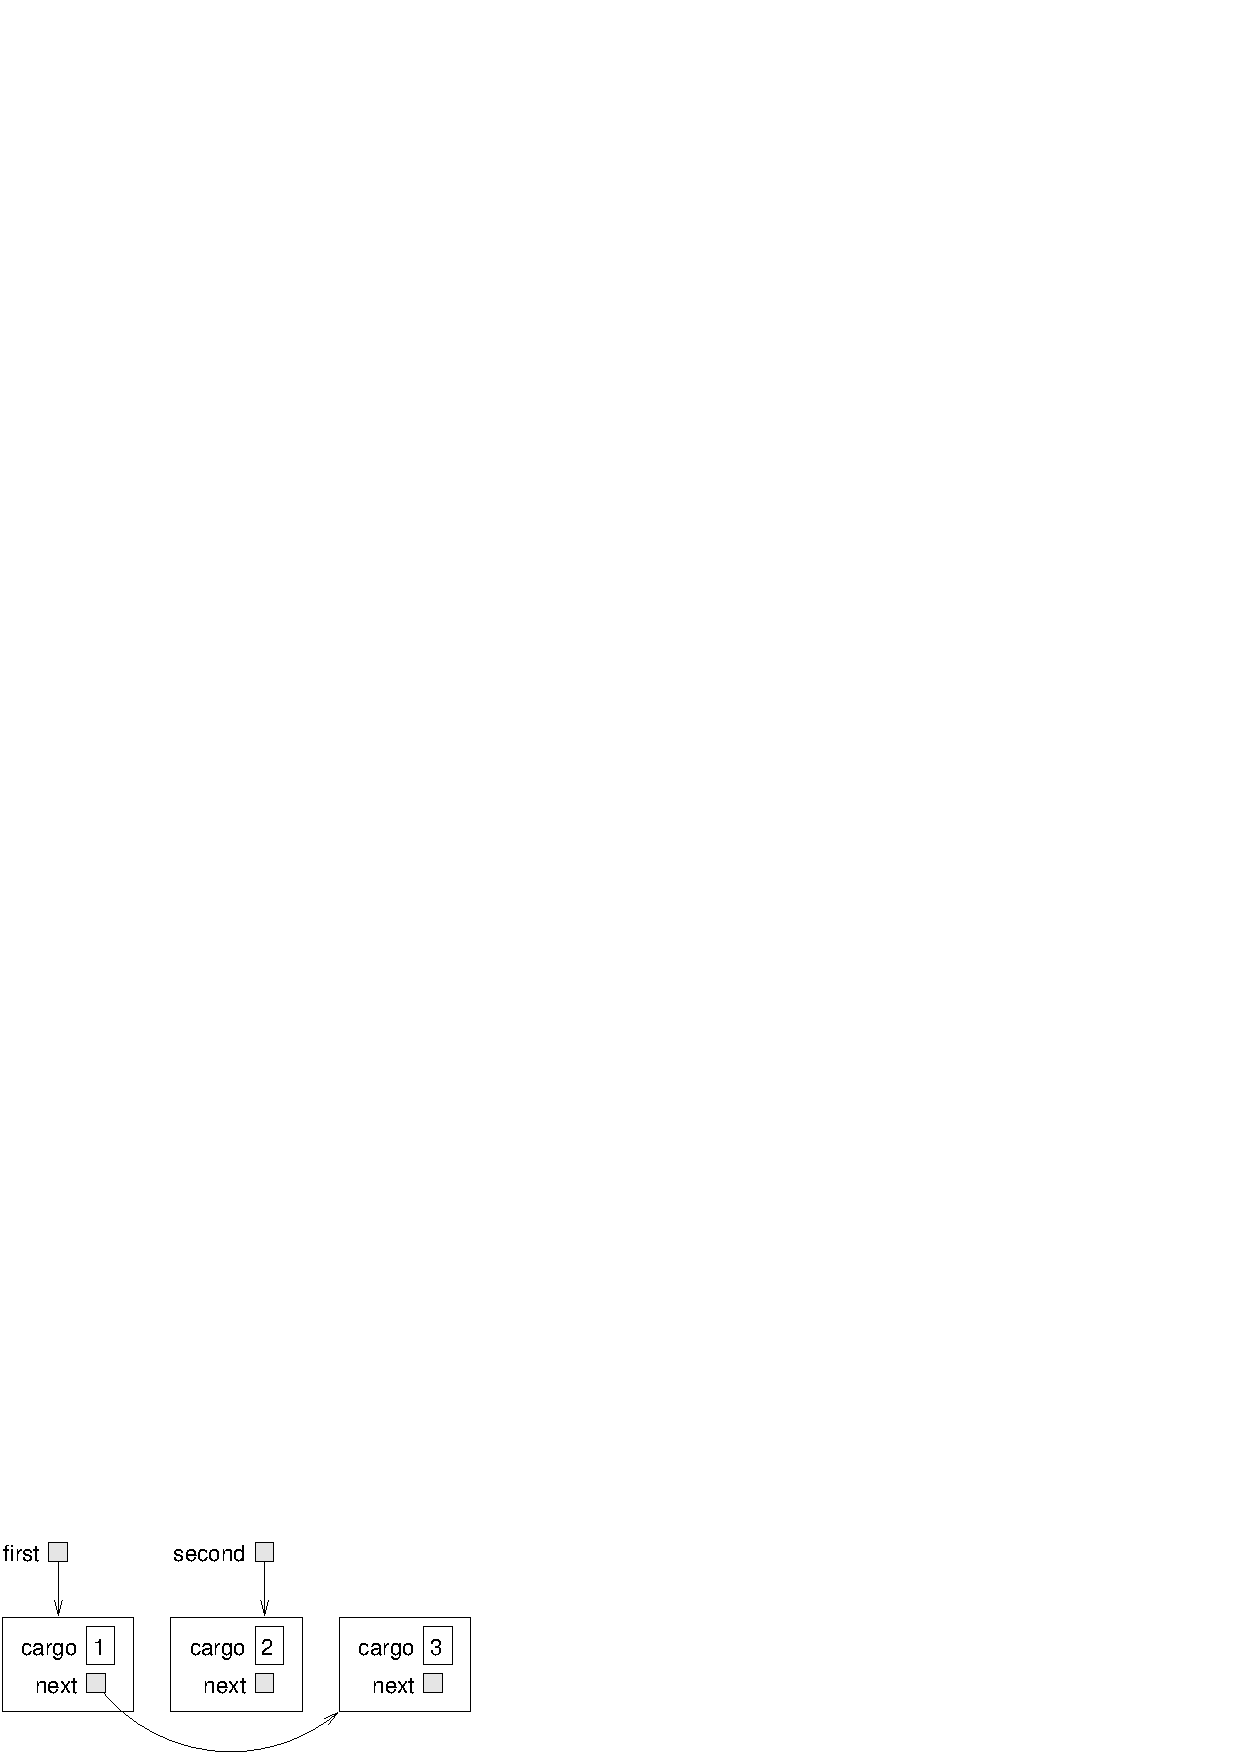
\includegraphics{figs/list5.pdf}

What happens if we invoke this method and pass a list with only one
element (a {\bf singleton})?  What happens if we pass the empty list
as an argument?  Is there a precondition for this method?

\index{singleton}


\section{Wrappers and helpers}
\label{wrapper}
\index{wrapper methods}
\index{method!wrapper}
\index{helper method}
\index{method!helper}

For some list operations it is useful to divide the labor into
two methods.  For example, to print a list backwards in the
conventional list format, {\tt (3, 2, 1)} we can use the
{\tt printBackwards} method to print {\tt 3, 2,} but we need
a separate method to print the parentheses and the first node.
We'll call it {\tt printBackwardNicely}.

\begin{verbatim}
    public static void printBackwardNicely (Node list) {
        System.out.print ("(");

        if (list != null) {
            Node head = list;
            Node tail = list.next;
            printBackward (tail);
            System.out.print (head);
        }
        System.out.println (")");
    }	
\end{verbatim}
%
Again, it is a good idea to check methods like this to see
if they work with special cases like an empty list or
a singleton.

\index{singleton}

Elsewhere in the program, when we use this method, we will
invoke {\tt printBackwardNicely} directly and it will invoke
{\tt printBackward} on our behalf.  In that sense, 
{\tt printBackwardNicely} acts as a {\bf wrapper}, and it uses
{\tt printBackward} as a helper.


\section {The {\tt IntList} class}
\index{IntList}
\index{class!IntList}

There are a number of subtle problems with the way we have been
implementing lists.  In a reversal of cause and effect, I will
propose an alternative implementation first and then explain what
problems it solves.

First, we will create a new class called {\tt IntList}.  Its
instance variables are an integer that contains the length of the list
and a reference to the first node in the list.  IntList objects
serve as handles for manipulating lists of Node objects.

\begin{verbatim}
public class IntList {
    int length;
    Node head;

    public IntList () {
        length = 0;
        head = null;
    }
}
\end{verbatim}
%
One nice thing about the {\tt IntList} class is that it gives
us a natural place to put wrapper functions like
{\tt printBackwardNicely}, which we can make an object
method in the {\tt IntList} class.

\begin{verbatim}
    public void printBackward () {
        System.out.print ("(");

        if (head != null) {
            Node tail = head.next;
            Node.printBackward (tail);
            System.out.print (head);
        }
        System.out.println (")");
    }	
\end{verbatim}
%
Just to make things confusing, I renamed {\tt printBackwardNicely}.
Now there are two methods named {\tt printBackward}: one in the
{\tt Node} class (the helper) and one in the {\tt IntList} class
(the wrapper).  In order for the wrapper to invoke the helper, it has
to identify the class explicitly ({\tt Node.printBackward}).

So, one of the benefits of the {\tt IntList} class is that
it provides a nice place to put wrapper functions.
Another is that it makes it easier to add or remove
the first element of a list.  For example, {\tt addFirst}
is an object method for {\tt IntLists}; it
takes an {\tt int} as an argument and puts it at the beginning of
the list.

\begin{verbatim}
    public void addFirst (int i) {
        Node node = new Node (i, head);
        head = node;
        length++;
    }
\end{verbatim}
%
As always, to check code like this it is a good idea to think about
the special cases.  For example, what happens if the list is initially
empty?


\section {Invariants}
\index{invariant}
\index{object invariant}
\index{list!well-formed}

Some lists are ``well-formed;'' others are not.  For example, if
a list contains a loop, it will cause many of our methods to
crash, so we might want to require that lists contain no loops.
Another requirement is that the {\tt length} value in the {\tt IntList}
object should be equal to the actual number of nodes in the list.

Requirements like this are called {\bf invariants} because, ideally,
they should be true of every object all the time.  Specifying invariants
for objects is a useful programming practice because it makes it
easier to prove the correctness of code, check the integrity of
data structures, and detect errors.

One thing that is sometimes confusing about invariants is that
there are some times when they are violated.  For example, in the
middle of {\tt addFirst}, after we have added the node, but
before we have incremented {\tt length}, the invariant is
violated.  This kind of violation is acceptable; in fact, it is
often impossible to modify an object without violating an
invariant for at least a little while.  Normally the requirement
is that every method that violates an invariant must restore
the invariant.

If there is any significant stretch of code in which the invariant
is violated, it is important for the comments to make that clear,
so that no operations are performed that depend on the invariant.

\index{documentation}


\section{Glossary}
\index{list}
\index{node}
\index{cargo}
\index{link}
\index{generic data structure}
\index{precondition}
\index{invariant}
\index{wrapper}

\begin{description}

\item[list:] A data structure that implements a collection using
a sequence of linked nodes.

\item[node:] An element of a list, usually implemented as an object
that contains a reference to another object of the same type.

\item[cargo:] An item of data contained in a node. 

\item[link:] An object reference embedded in an object.

\item[generic data structure:] A kind of data structure that can contain data
of any type.

\item[precondition:] An assertion that must be true in order for a
method to work correctly.

\item[invariant:] An assertion that should be true of an object at
all times (except maybe while the object is being modified).

\item[wrapper method:] A method that acts as a middle-man between a
caller and a helper method, often offering an interface that is
cleaner than the helper method's.

\end{description}


\section{Exercises}

\begin{exercise}
\label{ex.list}

Start by downloading the file {\tt IntList.java} from
\url{http://thinkapjava.com/code/IntList}.  It contains
the definitions of {\tt IntList} and {\tt Node} from this chapter,
along with code that demonstrates and tests some of the methods.
Compile and run the program.  The output should look like this:

\begin{verbatim}
(1, 2, 3)
(3, 2, 1)
\end{verbatim}

The following exercises ask you to write additional object
methods in the {\tt IntList}
class, but you might want to write some helper methods in the {\tt
Node} class as well.

After you write each method, add code to {\tt main}
and test it.  Be sure to test special cases like empty lists and
singletons.

For each method, identify any preconditions that are necessary
for the method to work and add comments that document them.  Your
comments should also indicate whether each method is a constructor,
function, or modifier.

\begin{enumerate}

\item Write a method named {\tt removeFirst} that removes
the first node from a list and returns its cargo.

\item Write a method named {\tt set} that takes an index, {\tt i}, and
an item of cargo, and that replaces the cargo of the {\tt i}th node
with the given cargo.

\item Write a method named {\tt add} that takes an index, {\tt i}, and
an item of cargo, and that adds a new node containing the given cargo
in the {\tt i}th position.

% \item Write a method called {\tt clone} that returns a new {\tt
% IntList} that contains all the same cargo as the original list, but
% it should contain all new {\tt Node} objects.  You might want to write
% a helper method in {\tt Node} to copy the nodes and link up the
% copies.  You might find it natural to write that method
% recursively.

% WARNING: There is already a method in the {\tt Object} class called
% {\tt clone}, which your method will override.  In order to do that,
% the return type has to be {\tt Object}, not {\tt IntList}.  Therefore,
% when you invoke {\tt clone}, you will have to cast the result to
% be an {\tt IntList} again.

\item Write a method named {\tt addLast} that takes an item of
cargo and adds it to the end of the list.

\item Write a method called {\tt reverse} that modifies an {\tt
IntList}, reversing the order of the nodes.

\item Write a method named {\tt append} that takes an {\tt IntList}
as a parameter and appends a {\em copy} of the nodes from the
parameter list onto the current list.  You should be able to take
advantage of code you have already written.

\item Write a method named {\tt checkLength} that returns true if the
length field equals the number of nodes in the list, and false
otherwise.  The method should not cause an exception under any
circumstances, and it should terminate even if the list contains a
loop.

\end{enumerate}
\end{exercise}


\begin{exercise}
One way to represent very large numbers is with a list of digits,
usually stored in reverse order.  For example, the number 123 might
be represented with the list $(3, 2, 1)$.

Write a method that compares two numbers represented as IntLists
and returns 1 if the first is larger, -1 if the second is larger, and
0 if they are equal.
\end{exercise}



\chapter{Stacks}

\section{Abstract data types}
\index{abstract data type|see{ADT}}
\index{ADT}
\index{encapsulation}

The data types we have looked at so far are all concrete, in the
sense that we have completely specified how they are implemented.
For example, the {\tt Card} class represents a card using two
integers.  As I discussed at the time, that is not the only way
to represent a card; there are many alternative implementations.

An {\bf abstract data type}, or ADT, specifies a set of operations (or
methods) and the semantics of the operations (what they do) but it
does not specify the implementation of the operations.  That's
what makes it abstract.

Why is that useful?

\begin{itemize}

\item It simplifies the task of specifying an algorithm if you
can denote the operations you need without having to think at the
same time about how the operations are performed.

\item Since there are usually many ways to implement an ADT,
it might be useful to write an algorithm that can be used with
any of the possible implementations.

\item Well-known ADTs, like the {\tt Stack} ADT in this chapter,
are often implemented in standard libraries so they can be written
once and used by many programmers.

\item The operations on ADTs provide a common high-level language
for specifying and talking about algorithms.

\end{itemize}

When we talk about ADTs, we often distinguish the code that uses
the ADT, called the {\bf client} code, from the code that implements
the ADT, called {\bf provider} code because it provides a standard
set of services.

\index{client}
\index{provider}


\section{The Stack ADT}
\index{stack}
\index{collection}
\index{ADT!Stack}

In this chapter we will look at one common ADT, the stack.  A
stack is a collection, meaning that it is a data structure that
contains multiple elements.  Other collections we have seen include
arrays and lists.

As I said, an ADT is defined by a set of operations.
Stacks can perform the following set of operations:

\begin{description}

\item[constructor:] Create a new, empty stack.

\item[{\tt push}:] Add a new item to the stack.

\item[{\tt pop}:] Remove and return an item from the stack.  The item
that is returned is always the last one that was added.

\item[{\tt isEmpty}:] Check whether the stack is empty.

\end{description}

A stack is sometimes called a ``last in, first out,'' or LIFO
data structure, because the last item added is the first to
be removed.


\section {The Java Stack Object}
\index{Stack}
\index{class!Stack}
\index{generic data structure}
\index{data structure!generic}

Java provides a built-in object type called {\tt Stack} that
implements the Stack ADT.  You should make some effort to keep
these two things---the ADT and the Java implementation---straight.
Before using the {\tt Stack} class, we have to import it from
{\tt java.util}.

Then the syntax for constructing a new {\tt Stack} is

\begin{verbatim}
    Stack stack = new Stack ();
\end{verbatim}
%
Initially the stack is empty, as we can confirm with the
{\tt isEmpty} method, which returns a {\tt boolean}:

\begin{verbatim}
    System.out.println (stack.isEmpty ());
\end{verbatim}
%
A stack is a generic data structure, which means that we can
add any type of item to it.  In the Java implementation, though,
we can only add object types.  For our first example, we'll
use {\tt Node} objects, as defined in the previous chapter.
Let's start by creating and printing a short list.

\begin{verbatim}
    IntList list = new IntList ();
    list.addFirst (3);
    list.addFirst (2);
    list.addFirst (1);
    list.print ();
\end{verbatim}
%
The output is {\tt (1, 2, 3)}.  To put a {\tt Node} object onto
the stack, use the {\tt push} method:

\begin{verbatim}
	stack.push (list.head);
\end{verbatim}
%
The following loop traverses the list and pushes all the nodes
onto the stack:

\begin{verbatim}
    for (Node node = list.head; node != null; node = node.next) {
        stack.push (node);
    }
\end{verbatim}
%
We can remove an element from the stack with the {\tt pop} method.

\begin{verbatim}
    Object obj = stack.pop ();
\end{verbatim}
%
The return type from {\tt pop} is {\tt Object}!  That's because the
stack implementation doesn't really know the type of the objects it
contains.  When we pushed the {\tt Node} objects, they were automatically
converted to {\tt Objects}.  When we get them back from the stack,
we have to cast them back to {\tt Nodes}.

\begin{verbatim}
Node node = (Node) obj;
System.out.println (node);
\end{verbatim}
%
Unfortunately, the burden falls on the programmer to keep track of the
objects in the stack and cast them back to the right type when they
are removed.  If you try to cast an object to the wrong type, you get
a {\tt ClassCastException}.

The following loop is a common idiom for popping all the elements
from a stack, stopping when it is empty:

\begin{verbatim}
    while (!stack.isEmpty ()) {
        Node node = (Node) stack.pop ();
        System.out.print (node + " ");
    }

\end{verbatim}
%
The output is {\tt 3 2 1}.  In other words, we just used a stack
to print the elements of a list backwards!  Granted, it's not the
standard format for printing a list, but using a stack it was
remarkably easy to do.

You should compare this code to the implementations of {\tt
printBackward} in the previous chapter.  There is a natural parallel
between the recursive version of {\tt printBackward} and the stack
algorithm here.  The difference is that {\tt printBackward} uses the
run-time stack to keep track of the nodes while it traverses the list,
and then prints them on the way back from the recursion.  The stack
algorithm does the same thing, just using a {\tt Stack} object instead
of the run-time stack.


\section {Wrapper classes}
\index{wrapper class}
\index{class!wrapper}
\index{object type}
\index{primitive type}

For every primitive type in Java, there is a built-in object type
called a {\bf wrapper class}.  For example, the wrapper class for
{\tt int} is called {\tt Integer}; for {\tt double} it is called
{\tt Double}.

Wrapper classes are useful for several reasons:

\begin{itemize}

\item You can instantiate wrapper classes and create objects
that contain primitive values.  In other words, you can wrap
a primitive value up in an object, which is useful if you want
to invoke a method that requires an object type.

\item Each wrapper class contains special values (like the
minimum and maximum values for the type), and methods that are useful
for converting between types.

\end{itemize}


\section {Creating wrapper objects}
\index{wrapper class!instantiating}

The most straightforward way to create a wrapper object is
to use its constructor:

\begin{verbatim}
    Integer i = new Integer (17);
    Double d = new Double (3.14159);
    Character c = new Character ('b');
\end{verbatim}
%
Technically {\tt String} is not a wrapper class, because there
is no corresponding primitive type, but the syntax for creating
a {\tt String} object is the same:

\begin{verbatim}
    String s = new String ("fred");
\end{verbatim}
%
On the other hand, no one ever uses the constructor for
{\tt String} objects, because you can get the same effect
with a simple {\tt String} value:

\begin{verbatim}
    String s = "fred";
\end{verbatim}


\section {Creating more wrapper objects}

Some of the wrapper classes have a second constructor that takes
a {\tt String} as an argument and tries to convert
to the appropriate type.  For example:

\begin{verbatim}
    Integer i = new Integer ("17");
    Double d = new Double ("3.14159");
\end{verbatim}
%
The type conversion process is not very robust.
For example, if the {\tt String}s are not in the right format,
they will cause a {\tt NumberFormatException}.  Any non-numeric
character in the {\tt String}, including a space, will cause
the conversion to fail.

\index{NumberFormatException}
\index{exception!NumberFormat}

\begin{verbatim}
    Integer i = new Integer ("17.1");        // WRONG!!
    Double d = new Double ("3.1459 ");       // WRONG!!
\end{verbatim}
%
It is usually a good idea to check the format of the {\tt String}
before you try to convert it.


\section{Getting the values out}
\index{wrapper class!extracting value}

Java knows how to print wrapper objects, so the easiest
way to extract a value is just to print the object:

\begin{verbatim}
    Integer i = new Integer (17);
    Double d = new Double (3.14159);
    System.out.println (i);
    System.out.println (d);
\end{verbatim}
%
Alternatively, you can use the {\tt toString} method to
convert the contents of the wrapper object to a String

\begin{verbatim}
    String istring = i.toString();
    String dstring = d.toString();
\end{verbatim}
%
Finally, if you just want to extract the primitive value
from the object, there is an object method in each wrapper
class that does the job:

\begin{verbatim}
    int iprim = i.intValue ();
    double dprim = d.doubleValue ();
\end{verbatim}
%
There are also methods for converting wrapper objects into
different primitive types.  You should check out the documentation
for each wrapper class to see what is available.


\section{Useful methods in the wrapper classes}
\index{wrapper class!methods}

As I mentioned, the wrapper classes contain useful methods that
pertain to each type.  For example, the {\tt Character} class contains
lots of methods for converting characters to upper and lower case, and
for checking whether a character is a number, letter, or symbol.

The {\tt String} class also contains methods for converting to upper
and lower case.  Keep in mind, though, that they are functions,
not modifiers (see Section~\ref{immutable}).

As another example, the {\tt Integer} class contains methods for
interpreting and printing integers in different bases.  If you have a
{\tt String} that contains a number in base 6, you can convert to base
10 using {\tt parseInt}.

\begin{verbatim}
    String base6 = "12345";
    int base10 = Integer.parseInt (base6, 6);
    System.out.println (base10);
\end{verbatim}
%
Since {\tt parseInt} is a class method, you invoke it by
naming the class and the method in dot notation.

Base 6 might not be all that useful, but hexadecimal
(base 16) and octal (base 8) are common for computer science
related things.


\section {Postfix expressions}
\index{postfix}
\index{infix}
\index{expressions}

In most programming languages, mathematical expressions are
written with the operator between the two operands, as in
{\tt 1+2}.  This format is called {\bf infix}.  An alternative
format used by some calculators is called {\bf postfix}.  In
postfix, the operator follows the operands, as in {\tt 1 2+}.

The reason postfix is sometimes useful is that there is a
natural way to evaluate a postfix expression using a stack.

\begin{itemize}

\item Starting at the beginning of the expression, get one
term (operator or operand) at a time.

	\begin{itemize}

	\item If the term is an operand, push it on the stack.

	\item If the term is an operator, pop two operands off
	the stack, perform the operation on them, and push the
	result back on the stack.

	\end{itemize}

\item When we get to the end of the expression, there should
be exactly one operand left on the stack.  That operand is the
result.

\end{itemize}

As an exercise, apply this algorithm to the expression
{\tt 1 2 + 3 *}.

This example demonstrates one of the advantages of postfix: there is
no need to use parentheses to control the order of operations.  To get
the same result in infix, we would have to write {\tt (1 + 2) * 3}.
As an exercise, write a postfix expression that is equivalent to {\tt
1 + 2 * 3}.


\section {Parsing}
\index{parse}
\index{token}
\index{delimiter}
\index{class!StringTokenizer}
\index{StringTokenizer class}

In order to implement the algorithm from the previous section,
we need to be able to traverse a string and break it into operands
and operators.  This process is an example of {\bf parsing}, and
the results---the individual chunks of the string---are called
{\bf tokens}.

Java provides a built-in class called a {\tt StringTokenizer}
that parses strings and breaks them into tokens.  To use it, you
have to import it from {\tt java.util}.

In its simplest form, the {\tt StringTokenizer} uses spaces
to mark the boundaries between tokens.  A character that marks
a boundary is called a {\bf delimiter}.

We can create a {\tt StringTokenizer} in the usual way, passing
as an argument the string we want to parse.

\begin{verbatim}
    StringTokenizer st = new StringTokenizer ("Here are four tokens.");
\end{verbatim}
%
The following loop is a standard idiom for extracting the tokens
from a {\tt StringTokenizer}.

\begin{verbatim}
    while (st.hasMoreTokens ()) {
        System.out.println (st.nextToken());
    }
\end{verbatim}
%
The output is

\begin{verbatim}
Here
are
four
tokens.
\end{verbatim}
%
For parsing expressions, we have the option of specifying additional
characters that will be used as delimiters:

\begin{verbatim}
    StringTokenizer st = new StringTokenizer ("11 22+33*", " +-*/");
\end{verbatim}
%
The second argument is a {\tt String} that contains all the characters
that will be used as delimiters.  Now the output is:

\begin{verbatim}
11
22
33
\end{verbatim}
%
This succeeds at extracting all the operands but we have lost the
operators.  Fortunately, there is one more option for {\tt
StringTokenizer}s.

\begin{verbatim}
    StringTokenizer st = new StringTokenizer ("11 22+33*", " +-*/", true);
\end{verbatim}
%
The third argument says, ``Yes, we would like to treat the delimiters
as tokens.''  Now the output is

\begin{verbatim}
11
 
22
+
33
*
\end{verbatim}
%
This is just the stream of tokens we would like for evaluating
this expression.


\section {Implementing ADTs}
\index{encapsulation}
\index{ADT}

One of the fundamental goals of an ADT is to separate the
interests of the provider, who writes the code that implements
the ADT, and the client, who uses the ADT.
The provider only has to worry
about whether the implementation is correct---in accord
with the specification of the ADT---and not how it will be used.

Conversely, the client {\em assumes} that the implementation of the
ADT is correct and doesn't worry about the details.  When you
are using one of Java's built-in classes, you have the luxury
of thinking exclusively as a client.

When you implement an ADT, on the other hand, you also have
to write client code to test it.  In that case, you sometimes
have to think carefully about which role you are playing at
a given instant.

In the next few sections we will switch gears and look at one way of
implementing the Stack ADT, using an array.  Start thinking like a
provider.


\section {Array implementation of the Stack ADT}
\label{arraystack}
\index{implementation!Stack}
\index{stack!array implementation}

The instance variables for this implementation are
an array of {\tt Objects}, which will contain the items on
the stack, and an integer index which will keep track of
the next available space in the array.
Initially, the array is empty and the index is {\tt 0}.

To add an element to the stack ({\tt push}), we'll copy 
a reference to it onto the stack and increment the index.
To remove an element ({\tt pop}) we have to decrement the
index first and then copy the element out.

Here is the class definition:

\begin{verbatim}
public class Stack {
    Object[] array;
    int index;

    public Stack () {
        this.array = new Object[128];
        this.index = 0;
    }
}
\end{verbatim}
%
As usual, once we have chosen the instance variables, it is
a mechanical process to write a constructor.
For now, the default size is 128 items.  Later we will consider
better ways of handling this.

Checking for an empty stack is trivial.

\begin{verbatim}
    public boolean isEmpty () {
        return index == 0;
    }
\end{verbatim}
%
It is important to remember, though, that the number of elements in
the stack is not the same as the size of the array.  Initially the
size is 128, but the number of elements is 0.

The implementations of {\tt push} and {\tt pop} follow naturally from
the specification.

\begin{verbatim}
    public void push (Object item) {
        array[index] = item;
        index++;
    }

    public Object pop () {
        index--;
        return array[index];
    }
\end{verbatim}
%
To test these methods, we can take advantage of the client code
we used to exercise the built-in Stack.  All we have to do is
comment out the line {\tt import java.util.Stack}.  Then, instead
of using the stack implementation from {\tt java.util} the
program will use the implementation we just wrote.

If everything goes according to plan, the program should
work without any additional changes.  Again, one of the strengths
of using an ADT is that you can change implementations without
changing client code.


\section{Resizing arrays}
\label{resize}
\index{array!resizing}
\index{ArrayIndexOutOfBounds}
\index{exception!ArrayIndexOutOfBounds}

A weakness of this implementation is that it chooses
an arbitrary size for the array when the {\tt Stack} is created.  If
the user pushes more than 128 items onto the stack, it will cause
an {\tt ArrayIndexOutOfBounds} exception.

\index{ArrayIndexOutOfBounds}
\index{exception!ArrayIndexOutOfBounds}

An alternative is to let the client code specify the size of
the array.  This alleviates the problem, but it requires the client
to know ahead of time how many items are needed, and that is not
always possible.

A better solution is to check whether the array is full and make
it bigger when necessary.  Since we have no idea how big the
array needs to be, it is a reasonable strategy to start with a
small size and double it each time it overflows.

Here's the improved version of {\tt push}:

\begin{verbatim}
    public void push (Object item) {
        if (full ()) resize ();

        // at this point we can prove that index < array.length

        array[index] = item;
        index++;
    }
\end{verbatim}
%
Before putting the new item in the array, we check if the array
is full.  If so, we invoke {\tt resize}.  After the {\tt if} statement,
we know that either (1) there was room in the array, or (2) the
array has been resized and there is room.  If {\tt full} and
{\tt resize} are
correct, then we can prove that {\tt index < array.length}, and 
therefore the next statement cannot cause an exception.

Now all we have to do is implement {\tt full} and {\tt resize}.

\begin{verbatim}
    private boolean full () {
        return index == array.length;
    }

    private void resize () {
        Object[] newArray = new Object[array.length * 2];

        // we assume that the old array is full
        for (int i=0; i<array.length; i++) {
            newArray[i] = array[i];
        }
        array = newArray;
    }
\end{verbatim}
%
Both methods are declared {\tt private}, which means that they
cannot be invoked from another class, only from
within this one.  This is acceptable, since there is no reason
for client code to use these functions, and desirable, since
it enforces the boundary between the provider code and the
client.

\index{method!private}
\index{private method}

The implementation of {\tt full} is trivial; it just checks
whether the index has gone beyond the range of valid indices.

The implementation of {\tt resize} is straightforward, with
the caveat that it assumes that the old array is full.  In other
words, that assumption is a precondition of this method.  It is
easy to see that this precondition is satisfied, since the only
way {\tt resize} is invoked is if {\tt full} returns true,
which can only happen if {\tt index == array.length}.

At the end of {\tt resize}, we replace the old array with
the new (causing the old to be garbage collected).  The
new {\tt array.length} is twice as big as the old, and 
{\tt index} hasn't changed, so now it must be true that
{\tt index < array.length}.  This assertion is a {\bf postcondition}
of {\tt resize}: something that must be true when the method
is complete (as long as its preconditions were satisfied).

Preconditions, postconditions, and invariants are useful tools
for analyzing programs and demonstrating their correctness.
In this example I have demonstrated a programming style that
facilitates program analysis and a style of documentation that
helps demonstrate correctness.

\index{precondition}
\index{postcondition}
\index{invariant}

\section{Glossary}
\index{ADT}
\index{client}
\index{provider}
\index{wrapper class}
\index{infix}
\index{postfix}
\index{parse}
\index{token}
\index{delimiter}
\index{predicate}
\index{postcondition}

\begin{description}

\item[abstract data type (ADT):]  A data type (usually a collection
of objects) that is defined by a set of operations, but that can
be implemented in a variety of ways.

\item[client:]  A program that uses an ADT (or the person who wrote
the program).

\item[provider:]  The code that implements an ADT (or the person
who wrote it).

\item[wrapper class:]  One of the Java classes, like {\tt Double}
and {\tt Integer} that provide objects to contain primitive types,
and methods that operate on primitives.

\item[{\tt private}:]  A Java keyword that indicates that a method
or instance variable cannot be accessed from outside the current
class definition.

\item[infix:]  A way of writing mathematical expressions with the
operators between the operands.

\item[postfix:]  A way of writing mathematical expressions with the
operators after the operands.

\item[parse:]  To read a string of characters or tokens and analyze
their grammatical structure.

\item[token:]  A set of characters that are treated as a unit for
purposes of parsing, like the words in a natural language.

\item[delimiter:]  A character that is used to separate tokens,
like the punctuation in a natural language.

\item[predicate:]  A mathematical statement that is either true or
false.

\item[postcondition:]  A predicate that must be true at the end of
a method (provided that the preconditions were true at the
beginning).


\end{description}


\section{Exercises}

\begin{exercise}
Write a method named {\tt reverse} that takes an array of integers,
traverses the array pushing each item onto a stack, and then pops
the items off the stack, putting them back into the array in the
reverse of their original order.

The point of this exercise is to practice the mechanisms for creating
wrapper objects, pushing and popping objects, and typecasting generic
Objects to a specific type.
\end{exercise}


\begin{exercise}
This exercise is based on the solution to Exercise~\ref{ex.list}.
Start by making a copy of your implementation of {\tt IntList}
called {\tt LinkedList}.

\begin {enumerate}

\item Transform the linked list implementation into a generic list by
making the cargo an {\tt Object} instead of an integer.
Modify the test code accordingly and run the program.

\item Write a {\tt LinkedList} method called {\tt split} that takes a
{\tt String}, breaks it up into words (using spaces as delimiters), and
returns a list of {\tt Strings}, with one word per list node.
Your implementation should be efficient, meaning that it takes
time proportional to the number of words in the string.

\item Write a {\tt LinkedList} method named {\tt join} that
returns a String that contains
the String representation of each of the objects in the list, in the order
they appear, with spaces in between.

\item Write a {\tt toString} method for {\tt LinkedList}. 

\end{enumerate}
\end{exercise}


\begin{exercise}
Write an implementation of the Stack ADT using your {\tt LinkedList}
implementation as the underlying data structure.  There are two
general approaches to this: the Stack might contain a LinkedList
as an instance variable, or the Stack class might extend the
LinkedList class.  Choose whichever sounds better to you, or,
if you are feeling ambitious, implement both and compare them.
\end{exercise}


\begin{exercise}
Write a program called {\tt Balance.java} that reads a file
and checks that the parentheses {\tt ()} and brackets {\tt []}
and squiggly-braces {\tt \{\}} are balanced and nested correctly.

HINT: See Section~\ref{fileIO} for code that reads lines
from a file.
\end{exercise}


\begin{exercise}
Write a method called {\tt evalPostfix} that takes a String containing
a postfix expression and returns a double that contains the result.
You can use a StringTokenizer to parse the String and a Stack of
Doubles to evaluate the expression.
\end{exercise}

\begin{exercise}
Write a program that prompts the user for a mathematical
expression in postfix and that evaluates the expression and
prints the result.
The following steps are my suggestion for a program development
plan.

\begin {enumerate}

\item Write a program that prompts the user for input and prints the
input string, over and over, until the user types ``quit''.  See
Section~\ref{keyboard} for information about getting input from the
keyboard.  You can use the following code as a starter:

\begin{verbatim}
    public static void inputLoop () throws IOException {
        BufferedReader stdin =
            new BufferedReader (new InputStreamReader (System.in));
	
        while (true) {
            System.out.print ("=>");       // print a prompt
            String s = stdin.readLine();   // get input
            if (s == null) break;
            // check if s is "quit"
            // print s
        }
    }
\end{verbatim}

\item Identify helper methods you think will be useful, and
write and debug them in isolation.  Suggestions: {\tt isOperator},
{\tt isOperand}, {\tt parseExpression}, {\tt performOperation}.

\item We know we want to push {\tt int} values onto the stack
and pop them off, which means we will have to use a wrapper class.
Make sure you know how to do that, and test those operations in
isolation.  Maybe make them helper methods.

\item Write a version of {\tt evaluate} that only handles one
kind of operator (like addition).  Test it in isolation.

\item Connect your evaluator to your input/output loop.

\item Add the other operations.

\item Once you have code that works, you might want to evaluate
the structural design.  How should you divide the code into
classes?  What instance variables should the classes have?  What
parameters should be passed around?

\item In addition to making the design elegant, you should also
make the code bulletproof, meaning that is should not cause an
exception under any circumstances, even if the user types something
weird.

\end{enumerate}
\end{exercise}




\chapter{Queues and Priority Queues}
\label{queue}
\index{queue}
\index{ADT!Queue}
\index{priority queue}
\index{ADT!Priority Queue}
\index{FIFO}
\index{queueing discipline}
\index{priority queueing}

This chapter presents two ADTs: Queues and Priority Queues.
In real life a {\bf queue} is a line of customers waiting for service
of some kind.  In most cases, the first customer in line is the
next customer to be served.  There are exceptions, though.  For
example, at airports customers whose flight is leaving imminently
are sometimes taken from the middle of the queue.  Also, at
supermarkets a polite customer might let someone with only a
few items go first.

The rule that determines who goes next is called a 
{\bf queueing discipline}.  The simplest queueing discipline is
called {\bf FIFO}, for ``first-in-first-out.''  The most general
queueing discipline is {\bf priority queueing}, in which each customer
is assigned a priority, and the customer with the highest priority
goes first, regardless of the order of arrival.  The reason I
say this is the most general discipline is that the priority
can be based on anything: what time a flight leaves, how many
groceries the customer has, or how important the customer is.
Of course, not all queueing disciplines are ``fair,'' but
fairness is in the eye of the beholder.

The Queue ADT and the Priority Queue ADT have the same set
of operations and their interfaces are the same.  The difference
is in the semantics of the operations: a Queue uses the FIFO
policy, and a Priority Queue (as the name suggests) uses the
priority queueing policy.

As with most ADTs, there are a number of ways to implement queues.
Since a queue is a collection of items, we can use any of the basic
mechanisms for storing collections, including arrays and lists.
Our choice among them will be based in part on their performance---
how long it takes to perform the operations we want to perform---
and partly on ease of implementation.

\index{collection}


\section{The queue ADT}
\index{ADT!Queue}
\index{Queue ADT}
\index{implementation!Queue}
\index{queue!List implementation}

The queue ADT is defined by the following operations:

\begin{description}

\item[constructor:] Create a new, empty queue.

\item[{\tt add}:] Add a new item to the queue.

\item[{\tt remove}:] Remove and return an item from the queue.  The item
that is returned is the first one that was added.

\item[{\tt isEmpty}:] Check whether the queue is empty.

\end{description}

Here is an implementation of a generic Queue, based on the
built-in class {\tt java.util.LinkedList}:

\begin{verbatim}
public class Queue {
    private LinkedList list;

    public Queue () {
        list = new LinkedList ();
    }

    public boolean isEmpty () {
        return list.isEmpty ();
    }

    public void add (Object obj) {
        list.addLast (obj);
    }

    public Object remove () {
        return list.removeFirst ();
    }
}
\end{verbatim}
%
A queue object contains a single instance variable, which is
the list that implements it.  For each of the other methods,
all we have to do is invoke one of the methods from the
{\tt LinkedList} class.

We can write the same implementation a bit more concisely by taking
advantage of inheritance:

\begin{verbatim}
public class Queue extends LinkedList {

    public Object remove () {
        return removeFirst ();
    }
}
\end{verbatim}
%
Ok, it's a lot more concise!  Because {\tt Queue} extends {\tt LinkedList},
we inherit the constructor, {\tt isEmpty} and {\tt add}.  We also
inherit {\tt remove}, but the version of {\tt remove} we get from
the {\tt LinkedList} class doesn't do what we want; it removes
the {\em last} element in the list, not the first.  We fix that
by providing a new version of {\tt remove}, which {\bf overrides}
the version we inherited.

The choice between these implementations depends on several factors.
Inheritance can make an implementation more concise, as long as
there are methods in the parent class that are useful.  But it can
also make an implementation more difficult to read and debug, because
the methods for the new class are not in one place.  Also, it can
lead to unexpected behavior, because the new class inherits {\em all}
the methods from the parent class, not just the ones you need.
That means that the second version of {\tt Queue}
provides methods like {\tt removeLast} and {\tt clear} that
are not part of the Queue ADT.
The first implementation is safer;
by declaring a {\tt private}
instance variable, it prevents
clients from invoking methods on the {\tt LinkedList}.

\index{instance variable!private}
\index{private instance variable}


\section{Veneer}
\index{veneer}
\index{performance hazard}
\index{performance analysis}

By using a LinkedList to implement a Queue, we were able
to take advantage of existing code; the code we wrote just
translates LinkedList methods into Queue methods.
An implementation like this is called a {\bf veneer}.  In
real life, veneer is a thin coating of good quality wood used
in furniture-making to hide lower quality wood underneath.
Computer scientists use this metaphor to describe a small
piece of code that hides the details of an implementation and
provides a simpler, or more standard, interface.

The Queue example demonstrates one of the nice things about a
veneer, which is that it is easy to implement, and one of
the dangers of using a veneer, which is the {\bf performance
hazard}!

Normally when we invoke a method we are not concerned with the
details of its implementation.  But there is one ``detail''
we might want to know---the performance characteristics of the
method.  How long does it take, as a function of the number
of items in the list?

To answer that question, we have to know more about the
implementation.  If we assume that {\tt LinkedList} is really
implemented as a linked list, then the
implementation of {\tt removeFirst} probably looks something
like this:

\begin{verbatim}
    public Object removeFirst () {
        Object result = head;
        if (head != null) {
            head = head.next;
        }
        return result.cargo;
    }
\end{verbatim}
%
We assume that {\tt head} refers to the first node in the list,
and that each node contains {\tt cargo} and a reference to
the next node in the list.

There are no loops or function calls here, so the run time of this
method is pretty much the same every time.  Such a method is called a
{\bf constant time} operation.  In reality, the method might be
slightly faster when the list is empty, since it skips the body of the
conditional, but that difference is not significant.

\index{constant time}

The performance of {\tt addLast} is very different.  Here is
a hypothetical implementation:

\begin{verbatim}
    public void addLast (Object obj) {
        // special case: empty list
        if (head == null) {
            head = new Node (obj, null);
            return;
        }
        Node last;
        for (last = head; last.next != null; last = last.next) {
            // traverse the list to find the last node
        }
        last.next = new Node (obj, null);
    }
\end{verbatim}
%
The first conditional handles the special case of adding a new node to
an empty list.  In this case, again, the run time does not depend on
the length of the list.  In the general case, though, we have to
traverse the list to find the last element so we can make it refer to
the new node.

This traversal takes time proportional to the length of the
list.  Since the run time is a linear function of the length,
we would say that this method is {\bf linear time}.  Compared to
constant time, that's very bad. 

\index{linear time}


\section{Linked Queue}
\index{queue!linked implementation}
\index{linked queue}

We would like an implementation of the Queue ADT that can
perform all operations in constant time.  One way to
accomplish that is to implement a {\bf linked queue}, which
is similar to a linked list in the sense that it is made up
of zero or more linked {\tt Node} objects.  The difference
is that the queue
maintains a reference to both the first and the last node,
as shown in the figure.

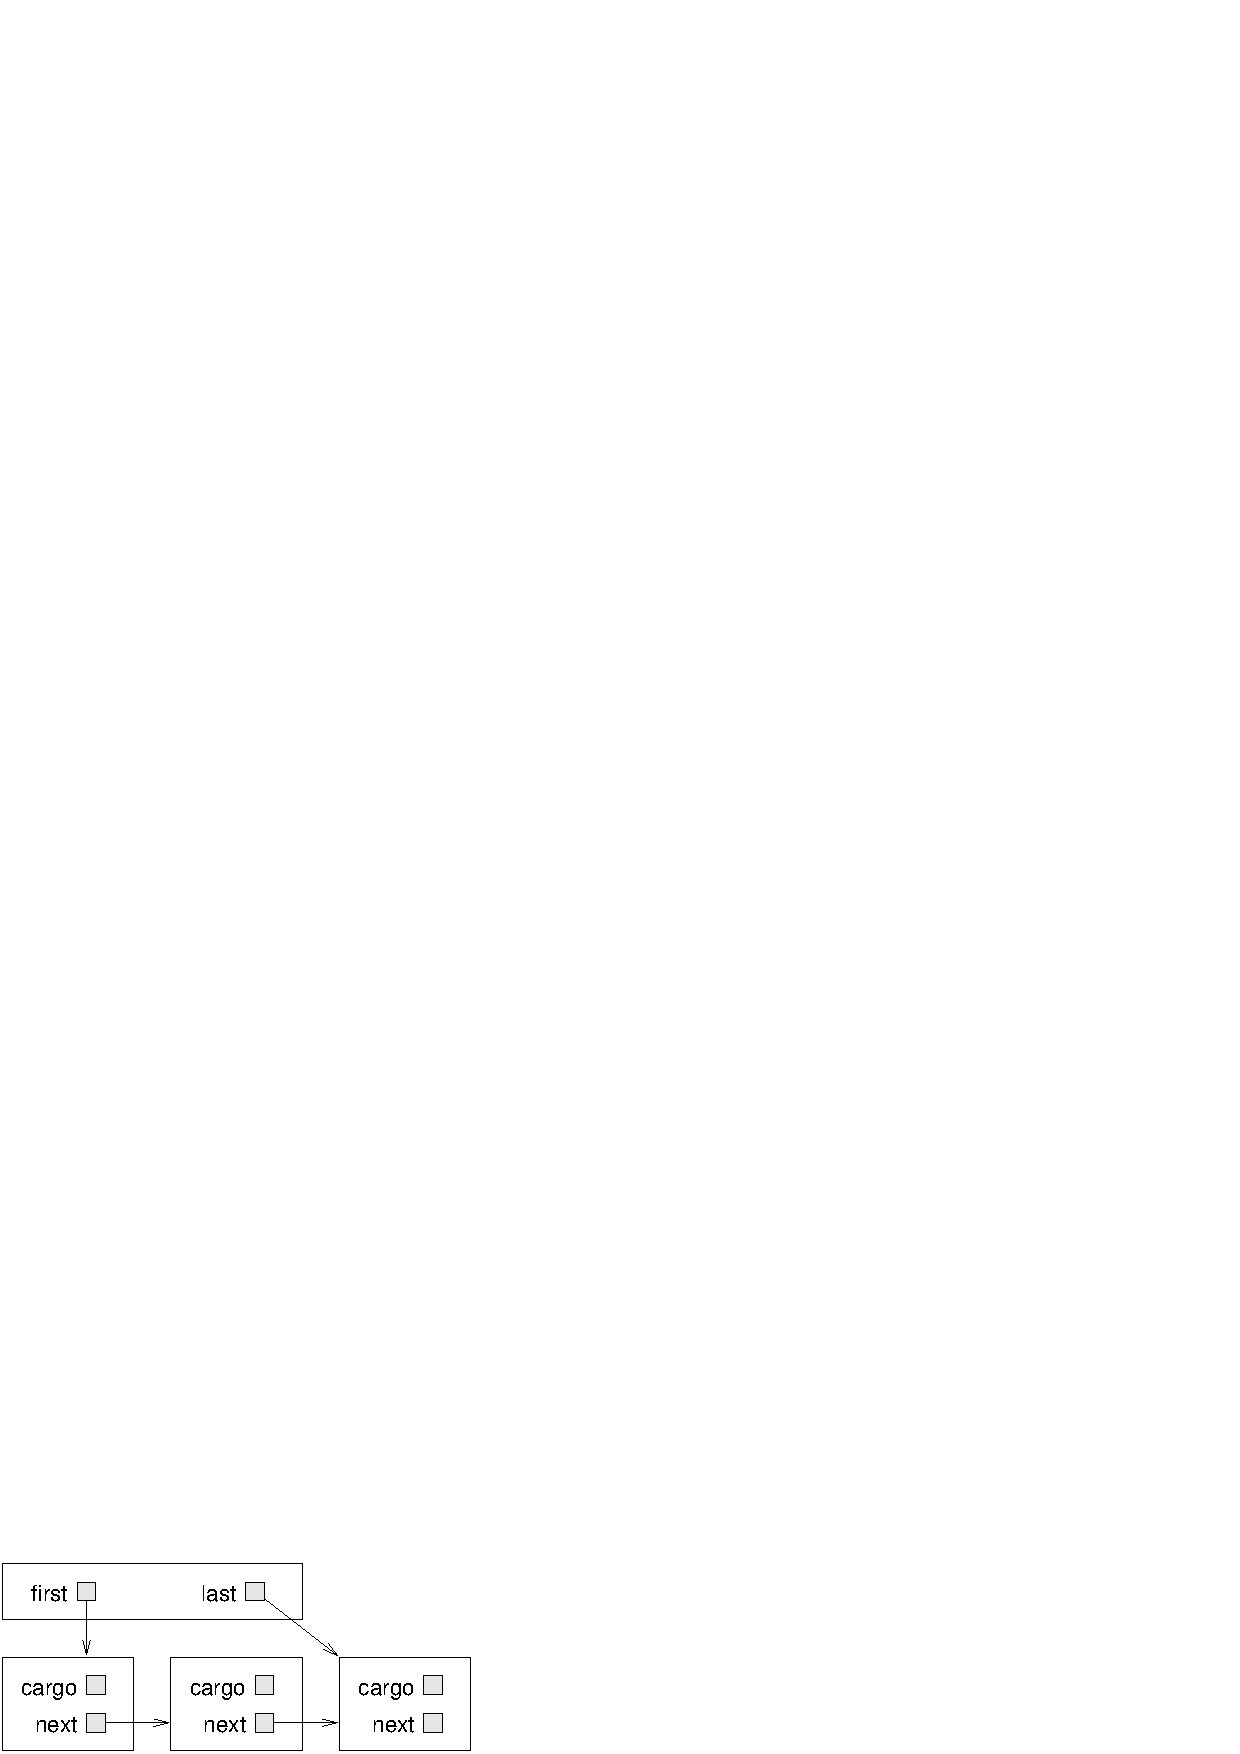
\includegraphics{figs/queue1.pdf}

Here's what a linked {\tt Queue} implementation looks like:

\begin{verbatim}
public class Queue {
    public Node first, last;

    public Queue () {
        first = null;
        last = null;
    }

    public boolean isEmpty () {
        return first == null;
    }
}
\end{verbatim}
%
So far it is straightforward.  In an empty queue, both {\tt first}
and {\tt last} are null.  To check whether a list is empty, we only
have to check one of them.

{\tt add} is a little more complicated because we have to
deal with several special cases.

\begin{verbatim}
    public void add (Object obj) {
        Node node = new Node (obj, null);
        if (last != null) {
            last.next = node;
        }
        last = node;
        if (first == null) {
            first = last;
        }
    }
\end{verbatim}
%
The first condition checks to make sure that {\tt last} refers
to a node; if it does then we have to make it refer to the new
node.

The second condition deals with the special case where the list
was initially empty.  In this case both {\tt first} and {\tt last}
refer to the new node.

{\tt remove} also deals with several special cases.

\begin{verbatim}
    public Object remove () {
        Node result = first;
        if (first != null) {
            first = first.next;
        }
        if (first == null) {
            last = null;
        }
        return result;
    }
\end{verbatim}
%
The first condition checks whether there were any nodes in
the queue.  If so, we have to copy the {\tt next} node into
{\tt first}.  The second condition deals with the special
case that the list is now empty, in which case we have to
make {\tt last} null.

As an exercise, draw diagrams showing these operations in
both the normal case and in the special cases, and convince
yourself that they are correct.

Clearly, this implementation is more complicated than the
veneer implementation, and it is more difficult to demonstrate
that it is correct.  The advantage is that we have achieved
the goal: {\tt add} and {\tt remove} are constant
time operations.


\section{Circular buffer}
\index{queue!circular buffer implementation}
\index{circular buffer}
\index{buffer!circular}

Another common implementation of a queue is a {\bf circular
buffer}.  ``Buffer'' is a general name for a temporary storage
location, although it often refers to an array, as it does in
this case.  What it means to say a buffer is ``circular'' should
become clear in a minute.

The implementation of a circular buffer is similar to the array
implementation of a stack in Section~\ref{arraystack}.  The
queue items are stored in an array, and we use indices to
keep track of where we are in the array.  In the stack implementation,
there was a single index that pointed to the next available space.
In the queue implementation, there are two indices: {\tt first}
points to the space in the array that contains the first customer
in line and {\tt next} points to the next available space.

The following figure shows a queue with two items (represented
by dots).

\includegraphics{figs/queue2.pdf}

There are two ways to think of the variables {\tt first} and
{\tt last}.  Literally, they are integers, and their values are
shown in boxes on the right.  Abstractly, though, they are
indices of the array, and so they are often drawn as arrows
pointing to locations in the array.  The arrow representation is
convenient, but you should remember that the indices are not
references; they are just integers.

Here is an incomplete array implementation of a queue:

\begin{verbatim}
public class Queue {
    public Object[] array;
    public int first, next;

    public Queue () {
        array = new Object[128];
        first = 0;
        next = 0;
    }

    public boolean isEmpty () {
        return first == next;
    }
\end{verbatim}
%
The instance variables and the constructor are straightforward,
although again we have the problem that we have to choose an
arbitrary size for the array.  Later we will solve that problem,
as we did with the stack, by resizing the array if it gets full.

The implementation of {\tt isEmpty} is a little surprising.  You might
have thought that {\tt first == 0} would indicate an empty queue, but
that neglects the fact that the head of the queue is not necessarily
at the beginning of the array.  Instead, we know that the queue is
empty if {\tt head} equals {\tt next}, in which case there are no
items left.  Once we see the implementation of {\tt add} and {\tt
remove}, that condition will make more sense.

\begin{verbatim}
    public void add (Object item) {
        array[next] = item;
        next++;
    }

    public Object remove () {
        Object result = array[first];
        first++;
        return result;
    }
\end{verbatim}
%
{\tt add} looks very much like {\tt push} in Section~\ref{arraystack};
it puts the new item in the next available space and then increments
the index.

{\tt remove} is similar.  It takes the first item from the queue
and then increments {\tt first} so it refers to the new head of the queue.
The following figure shows what the queue looks like after both
items have been removed.

\includegraphics{figs/queue3.pdf}

It is always true that {\tt next} points to an available space.
If {\tt first} catches up with {\tt next} and points to the same
space, then {\tt first} is referring to an ``empty'' location,
and the queue is empty.  I put ``empty'' in quotation marks because
it is possible that the location that {\tt first} points to actually
contains a value (we do nothing to ensure that empty locations contain
{\tt null}); on the other hand, since we know the queue is empty, we
will never read this location, so we can think of it, abstractly,
as empty.

\begin{exercise}
Modify {\tt remove} so that it returns {\tt null}
if the queue is empty.
\end{exercise}

The next problem with this implementation is that eventually it
will run out of space.  When we add an item we increment {\tt next}
and when we remove an item we increment {\tt first}, but we never
decrement either.  What happens when we get to the end of the
array?

The following figure shows the queue after we add four more items:

\includegraphics{figs/queue4.pdf}

The array is now full.  There is no ``next available space,'' so there
is nowhere for {\tt next} to point.  One possibility is that we could
resize the array, as we did with the stack implementation.  But in that
case the array would keep getting bigger regardless of how many items
were actually in queue.  A better solution is to wrap around to the
beginning of the array and reuse the spaces there.  This ``wrap around''
is the reason this implementation is called a circular buffer.

One way to wrap the index around is to add a special case whenever
we increment an index:

\begin{verbatim}
        next++;
        if (next == array.length) next = 0; 
\end{verbatim}
%
A fancy alternative is to use the modulus operator:

\begin{verbatim}
        next = (next + 1) % array.length;
\end{verbatim}
%
Either way, we have one last problem to solve.  How do we know
if the queue is {\em really} full, meaning that we cannot add
another item?  The following figure shows what the queue looks
like when it is ``full.''

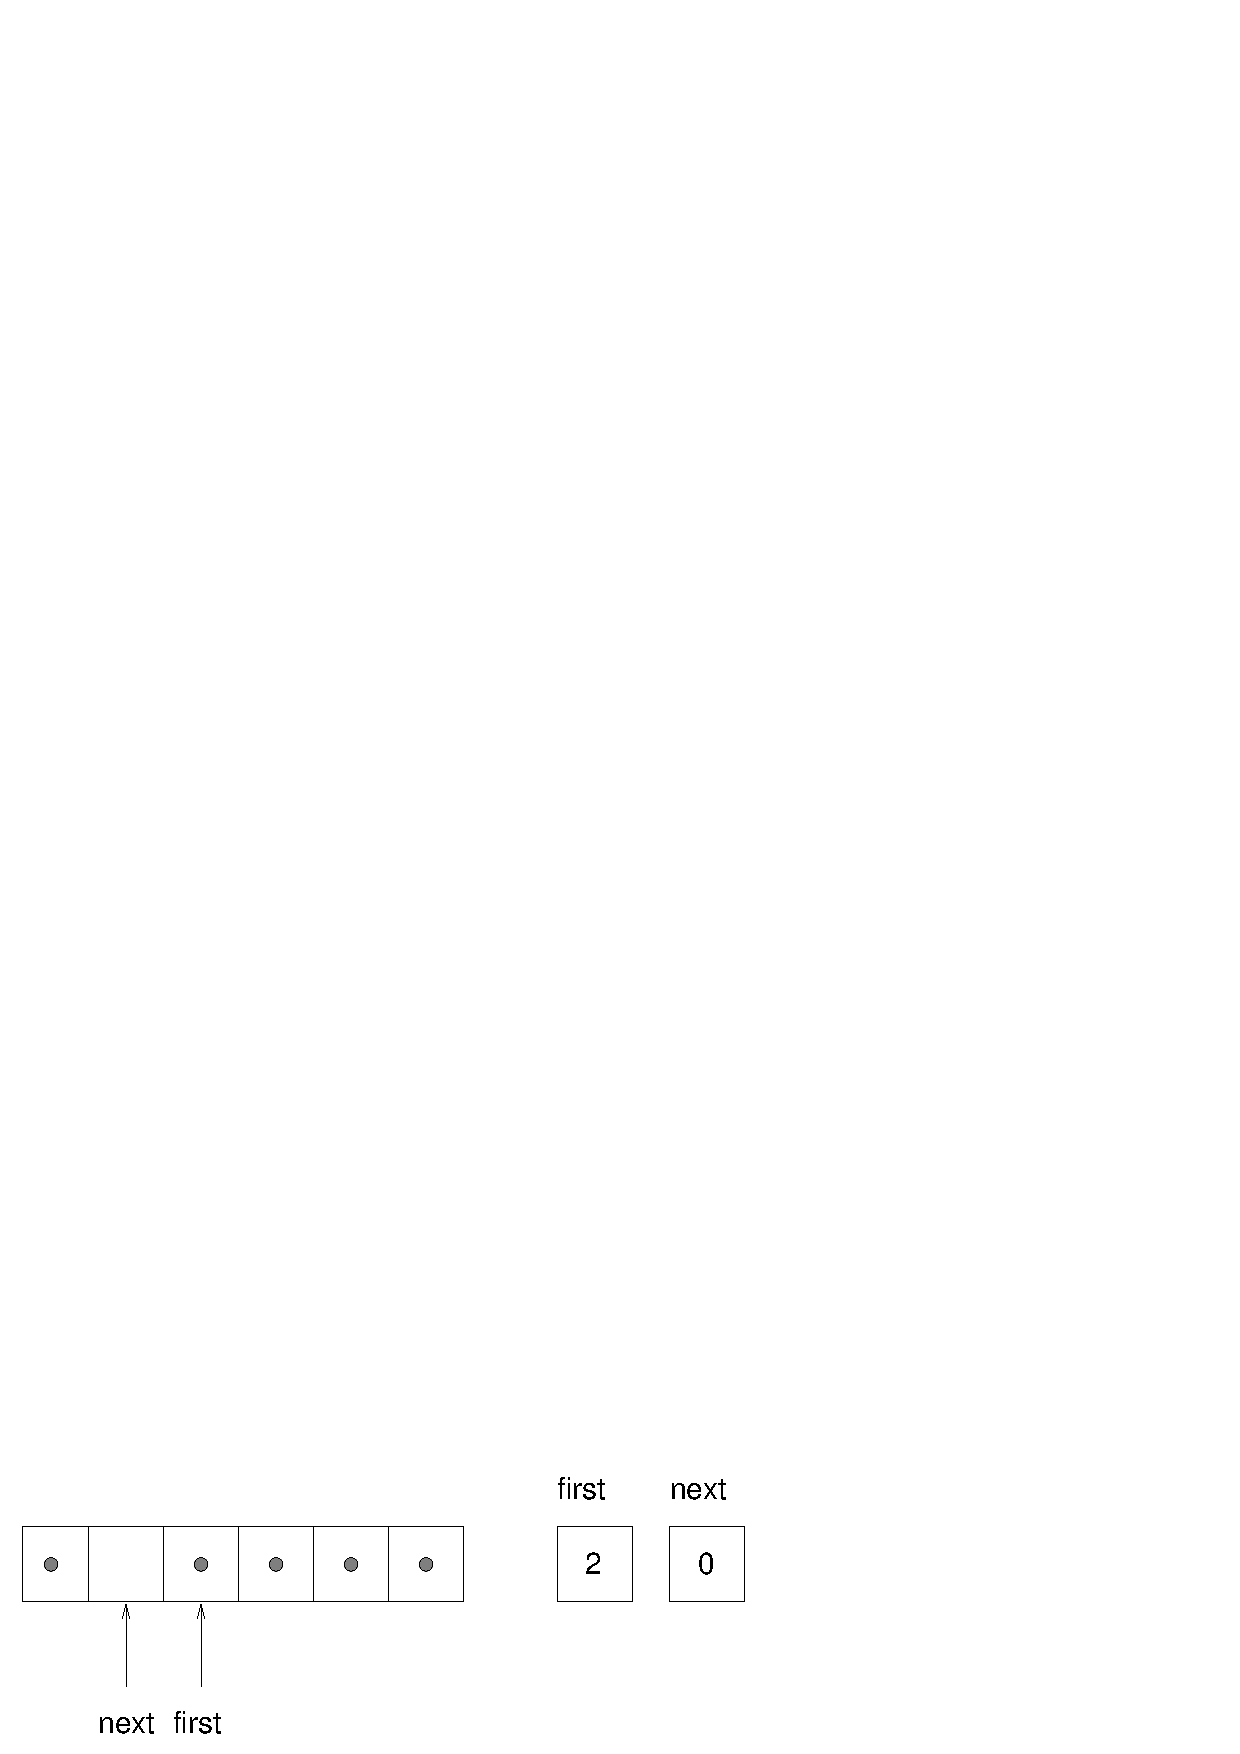
\includegraphics{figs/queue5.pdf}

There is still one empty space in the array, but the queue is
full because if we add another item, then we have to increment
{\tt next} such that {\tt next == first}, and in that case it
would appear that the queue was empty!

To avoid that, we sacrifice one space in the array.  So how
can we tell if the queue is full?

\begin{verbatim}
        if ((next + 1) % array.length == first)
\end{verbatim}
%
And what should we do if the array is full?  In that case resizing
the array is probably the only option.

\begin{exercise}
Write an implementation of a queue using a circular buffer that
resizes itself when necessary.
\end{exercise}


\section{Priority queue}
\index{priority queue!ADT}
\index{ADT!Priority Queue}

The Priority Queue ADT has the same interface as
the Queue ADT, but different semantics.  The interface is:

\begin{description}

\item[constructor:] Create a new, empty queue.

\item[{\tt add}:] Add a new item to the queue.

\item[{\tt remove}:] Remove and return an item from the queue.  The item
that is returned is the one with the highest priority.

\item[{\tt isEmpty}:] Check whether the queue is empty.

\end{description}

The semantic difference is that the item that is removed from
the queue is not necessarily the first one that was added.  Rather,
it is whatever item in the queue has the highest priority.
What the priorities are, and how they compare to each other, are not
specified by the Priority Queue implementation.  It depends on
what the items are that are in the queue.

For example, if the items in the queue have names, we might choose
them in alphabetical order.  If they are bowling scores, we might
choose from highest to lowest, but if they are golf scores, we would
go from lowest to highest.

\index{generic}
\index{data structure!generic}

So we face a new problem.  We would like an implementation of
Priority Queue that is generic---it should work with any kind
of object---but at the same time the code that implements Priority
Queue needs to have the ability to compare the objects it contains.

We have seen a way to implement generic data structures using
{\tt Objects}, but that does not solve this problem, because
there is no way to compare {\tt Objects} unless we know what type
they are.

The answer lies in a Java feature called a {\bf metaclass}.


\section {Metaclass}
\index{metaclass}
\index{Comparable}
\index{metaclass!Comparable}

A metaclass is a set of classes that provide a common set of methods.
The metaclass definition specifies the requirements a class must
satisfy to be a member of the set.

Often metaclasses have names that end in ``able'' to indicate
the fundamental capability the metaclass requires.  For
example, any class that provides a method named {\tt draw} can
be a member of the metaclass named {\tt Drawable}.  Any
class that contains a method named {\tt start} can be a member
of the metaclass {\tt Runnable}.

Java provides a built-in metaclass that we can use in an
implementation of a Priority Queue.  It is called {\tt Comparable},
and it means what it says.  Any class that belongs to the {\tt
Comparable} metaclass has to provide a method named {\tt compareTo}
that compares two objects and returns a value indicating whether one
is larger or smaller than the other, or whether they are the same.

Many of the built-in Java classes are members of the {\tt Comparable}
metaclass, including numeric wrapper classes like {\tt Integer}
and {\tt Double}.

In the next section I will show how to write an ADT that manipulates
a metaclass.  Then we will see how to write a new
class that belongs to an existing metaclass.  In the
next chapter we will see how to define a new metaclass.


\section{Array implementation of Priority Queue}
\index{implementation!Priority Queue}
\index{priority queue!array implementation}

In the implementation of the Priority Queue, every time we specify
the type of the items in the queue, we specify the metaclass
{\tt Comparable}.  For example, the instance variables are an
array of {\tt Comparables} and an integer:

\begin{verbatim}
public class PriorityQueue {
    private Comparable[] array;
    private int index;
}
\end{verbatim}
%
As usual, {\tt index} is the index of the next available location in the
array.  The instance variables are declared {\tt private} so that
other classes cannot have direct access to them.

\index{instance variable!private}
\index{private instance variable}

The constructor and {\tt isEmpty} are similar to what we have seen
before.  The initial size of the array is arbitrary.

\begin{verbatim}
    public PriorityQueue () {
        array = new Comparable [16];
        index = 0;
    }

    public boolean isEmpty () {
        return index == 0;
    }
\end{verbatim}
%
{\tt add} is similar to {\tt push}:

\begin{verbatim}
    public void add (Comparable item) {
        if (index == array.length) {
            resize ();
        }
        array[index] = item;
        index++;
    }
\end{verbatim}
%
The only substantial method in the class is {\tt remove}, which has
to traverse the array to find and remove the largest item:

\begin{verbatim}
    public Comparable remove () {
        if (index == 0) return null;

        int maxIndex = 0;

        // find the index of the item with the highest priority
        for (int i=1; i<index; i++) {
            if (array[i].compareTo (array[maxIndex]) > 0) {
                maxIndex = i;
            }
        }
        Comparable result = array[maxIndex];

        // move the last item into the empty slot
        index--;
        array[maxIndex] = array[index];
        return result;
   }
\end{verbatim}
%
As we traverse the array, {\tt maxIndex} keeps track of the
index of the largest element we have seen so far.  What it
means to be the ``largest'' is determined by {\tt compareTo}.
In this case the {\tt compareTo} method is provided by the
{\tt Integer} class, and it does what we expect---larger
(more positive) numbers win.


\section {A Priority Queue client}
\index{client}
\index{metaclass}

The implementation of Priority Queue is written entirely
in terms of {\tt Comparable} objects, but there is no
such thing as a {\tt Comparable} object!  Go ahead, try
to create one:

\begin{verbatim}
    Comparable comp = new Comparable ();       // ERROR
\end{verbatim}
%
You'll get a compile-time message that says something like
``java.lang.Comparable is an interface.  It can't be instantiated.''
In Java, metaclasses are called {\bf interfaces}.  I have
avoided this word so far because it also means several other
things, but now you have to know.

\index{interface}

Why can't metaclasses be instantiated?  Because a metaclass
only specifies requirements (you must have a {\tt compareTo}
method); it does not provide an implementation.

To create a {\tt Comparable} object, you have to create one of the
objects that belongs to the {\tt Comparable} set, like {\tt Integer}.
Then you can use that object anywhere a {\tt Comparable} is called
for.

\begin{verbatim}
        PriorityQueue pq = new PriorityQueue ();
        Integer item = new Integer (17);
        pq.add (item);
\end{verbatim}
%
This code creates a new, empty Priority Queue and a new {\tt Integer}
object.  Then it adds the {\tt Integer} into the queue.  {\tt
add} is expecting a {\tt Comparable} as a parameter, so it is
perfectly happy to take an {\tt Integer}.  If we try to pass a {\tt
Rectangle}, which does not belong to {\tt Comparable}, we get a
compile-time message like, ``Incompatible type for method.  Explicit
cast needed to convert java.awt.Rectangle to java.lang.Comparable.''

That's the compiler telling us that if we want to make that conversion,
we have to do it explicitly.  We might try to do what it says:

\begin{verbatim}
	Rectangle rect = new Rectangle ();
	pq.add ((Comparable) rect);
\end{verbatim}
%
But in that case we get a run-time error, a {\tt ClassCastException}.
When the {\tt Rectangle} tries to pass as a {\tt Comparable}, the
run-time system checks whether it satisfies the requirements, and
rejects it.  So that's what we get for following the compiler's advice.

\index{ClassCastException}
\index{exception!ClassCastException}

To get items out of the queue, we have to reverse the process:

\begin{verbatim}
    while (!pq.isEmpty ()) {
        item = (Integer) pq.remove ();
        System.out.println (item);
    }
\end{verbatim}
%
This loop removes all the items from the queue and prints them.
It assumes that the items in the queue are {\tt Integers}.
If they were not, we would get a {\tt ClassCastException}.


\section{The {\tt Golfer} class}
\index{Golfer}
\index{class!Golfer}
\index{metaclass!implementing}
\index{Comparable}

Finally, let's look at how we can make a new class that belongs to
{\tt Comparable}.  As an example of something with an unusual definition
of ``highest'' priority, we'll use golfers:

\begin{verbatim}
public class Golfer implements Comparable {
    String name;
    int score;

    public Golfer (String name, int score) {
        this.name = name;
        this.score = score;
    }
}
\end{verbatim}
%
The class definition and the constructor are pretty much the same as
always; the difference is that we have to declare that {\tt Golfer
implements Comparable}.  In this case the keyword {\tt implements}
means that {\tt Golfer} implements the interface specified by {\tt
Comparable}.

If we try to compile {\tt Golfer.java} at
this point, we get something like ``class Golfer must be declared
abstract. It does not define int compareTo(java.lang.Object) from
interface java.lang.Comparable.''  In other words, to be a {\tt Comparable},
{\tt Golfer} has to provide a method named {\tt compareTo}.  So
let's write one:

\begin{verbatim}
    public int compareTo (Object obj) {
        Golfer that = (Golfer) obj;

        int a = this.score;
        int b = that.score;
	
        // for golfers, low is good!
        if (a<b) return 1;
        if (a>b) return -1;
        return 0;
    }
\end{verbatim}
%
Two things here are a little surprising.  First, the parameter
is an {\tt Object}.  That's because in general the caller doesn't
know what type the objects are that are being compared.  For
example, in {\tt PriorityQueue.java} when we invoke {\tt compareTo},
we pass a {\tt Comparable} as a parameter.  We don't have to
know whether it is an {\tt Integer} or a {\tt Golfer} or whatever.

Inside {\tt compareTo} we have to convert the parameter from
an {\tt Object} to a {\tt Golfer}.  As usual, there is a risk
when we do this kind of cast: if we cast to the wrong type we
get an exception.

Finally, we can create some golfers:

\begin{verbatim}
        Golfer tiger = new Golfer ("Tiger Woods", 61);
        Golfer phil = new Golfer ("Phil Mickelson", 72);
        Golfer hal = new Golfer ("Hal Sutton", 69);
\end{verbatim}
%
And put them in the queue:

\begin{verbatim}
        pq.add (tiger);
        pq.add (phil);
        pq.add (hal);
\end{verbatim}
%
When we pull them out:

\begin{verbatim}
        while (!pq.isEmpty ()) {
            golfer = (Golfer) pq.remove ();
            System.out.println (golfer);
        }
\end{verbatim}
%
They appear in descending order (for golfers):

\begin{verbatim}
        Tiger Woods     61
        Hal Sutton      69
        Phil Mickelson  72
\end{verbatim}
%
When we switched from {\tt Integers} to {\tt Golfers}, we didn't
have to make any changes in {\tt PriorityQueue.java} at all.  So
we succeeded in maintaining a barrier between {\tt PriorityQueue}
and the classes that use it, allowing us to reuse the code without
modification.  Furthermore, we were able to give the client code
control over the definition of {\tt compareTo}, making this
implementation of {\tt PriorityQueue} more versatile.



\section{Glossary}
\index{queue}
\index{queueing discipline}
\index{FIFO}
\index{priority queue}
\index{veneer}
\index{constant time}
\index{linear time}
\index{performance hazard}
\index{linked queue}
\index{circular buffer}
\index{metaclass}
\index{interface}

\begin{description}

\item[queue:]  An ordered set of objects waiting for a service of
some kind.

\item[queueing discipline:]  The rules that determine which member
of a queue is removed next.

\item[FIFO:]  ``first in, first out,'' a queueing discipline in which
the first member to arrive is the first to be removed.

\item[priority queue:]  A queueing discipline in which
each member has a priority determined by external factors.
The member with the highest priority is the first to be removed.

\item[Priority Queue:]  An ADT that defines the operations one
might perform on a priority queue.

\item[veneer:]  A class definition that implements an ADT with
method definitions that are invocations of other methods, sometimes
with simple transformations.  The veneer does no significant work,
but it improves or standardizes the interface seen by the client.

\item[performance hazard:]  A danger associated with a veneer that
some of the methods might be implemented inefficiently in a way
that is not apparent to the client.

\item[constant time:]  An operation whose run time does not
depend on the size of the data structure.

\item[linear time:]  An operation whose run time is a linear
function of the size of the data structure.

\item[linked queue:]  An implementation of a queue using a linked
list and references to the first and last nodes.

\item[circular buffer:]  An implementation of a queue using an
array and indices of the first element and the next available space.

\item[metaclass:]  A set of classes.  The metaclass specification
lists the requirements a class must satisfy to be included in the set.

\item[interface:]  The Java word for a metaclass.  Not to be
confused with the more broad meaning of the word interface.


\end{description}


\section{Exercises}

\begin{exercise}
This question is based on Exercise~\ref{ex.rational}.

Write a {\tt compareTo} method for the {\tt Rational} class
that would allow {\tt Rational} to implement {\tt Comparable}.
Hint: don't forget that the parameter is an {\tt Object}.
\end{exercise}


\begin{exercise}
Write a class definition for {\tt SortedList}, which extends
{\tt LinkedList}.  A SortedList is similar to a LinkedList; the
difference is that the elements have to be Comparable, and the
list is sorted in decreasing order.

Write an object method for {\tt SortedList}
called {\tt add} that takes a Comparable as a parameter and that
adds the new object into the list,
at the appropriate place so
that the list stays sorted.

If you want, you can write a helper method in the {\tt Node} class.
\end{exercise}


\begin{exercise}
Write an object method for the {\tt LinkedList} class
named {\tt maximum} that can be invoked on a
{\tt LinkedList} object, and that returns the largest cargo
object in the list, or null if the list is empty.

You can assume that every cargo element belongs to a class that
belongs to the metaclass {\tt Comparable}, and that any two
elements can be compared to each other.
\end{exercise}



\begin{exercise}
Write an implementation of a Priority Queue using
a linked list.  There are three ways you might proceed:

\begin{itemize}

\item A Priority Queue might contain a LinkedList object as an
instance variable.

\item A Priority Queue might contain a reference to the
first Node object in a linked list.

\item A Priority Queue might extend (inherit from) the existing
LinkedList class.

\end{itemize}
%
Think about the pros and cons of each and choose one.  Also, you
can choose whether to keep the list sorted (slow add, fast remove)
or unsorted (slow remove, fast add).
\end{exercise}


\begin{exercise}
An event queue is a data structure that keeps track of a set
of events, where each event has a time associated with it.
The ADT is:

\begin{description}

\item[constructor:] make a new, empty event queue

\item[{\tt add}:] put a new event in the queue.  The parameters are
the event, which is an Object, and the time the event occurs, which
is a {\tt Date} object.  The event Object must not be null.

\item[{\tt nextTime}:] return the {\tt Date} at which the next event
occurs, where the ``next'' event is the one in the queue with the
earliest time.  Do not remove the event from the queue.  Return
null if the queue is empty.

\item[{\tt nextEvent}:] return the next event (an {\tt Object}) from
the queue and remove it from the queue.  Return null if the queue is
empty.

%\item[{\tt events}:] return an {\tt Iterator} that includes all the
%events in the queue, ordered from lowest to highest.  Do not modify
%the queue.

\end{description}

The {\tt Date} class is defined in {\tt java.util} and it implements
{\tt Comparable}.  According to the documentation, its {\tt compareTo}
method returns ``the value 0 if the argument Date is equal to this
Date; a value less than 0 if this Date is before the Date argument;
and a value greater than 0 if this Date is after the Date argument.''

Write an implementation of an event queue using the PriorityQueue
ADT.  You should not make any assumptions about how the PriorityQueue
is implemented.

HINT: create a class named {\tt Event} that contains a {\tt Date}
and an event {\tt Object}, and that implements {\tt Comparable}
appropriately.
\end{exercise}



\chapter{Trees}
\index{tree}
\index{ADT}
\index{data structure}

\section{A tree node}
\index{node}
\index{tree node}
\index{cargo}
\index{embedded reference}
\index{implementation!Tree}
\index{binary tree}

Like lists, trees are made up of nodes.  A common kind of tree is
a {\bf binary tree}, in which each node contains a reference to two
other nodes (possibly null).  The class definition looks like this:

\begin{verbatim}
public class Tree {
    Object cargo;
    Tree left, right;
}
\end{verbatim}
%
Like list nodes, tree nodes contain cargo: in this case a generic {\tt
Object}.  The other instance variables are named {\tt left} and {\tt
right}, in accordance with a standard way to represent trees
graphically:

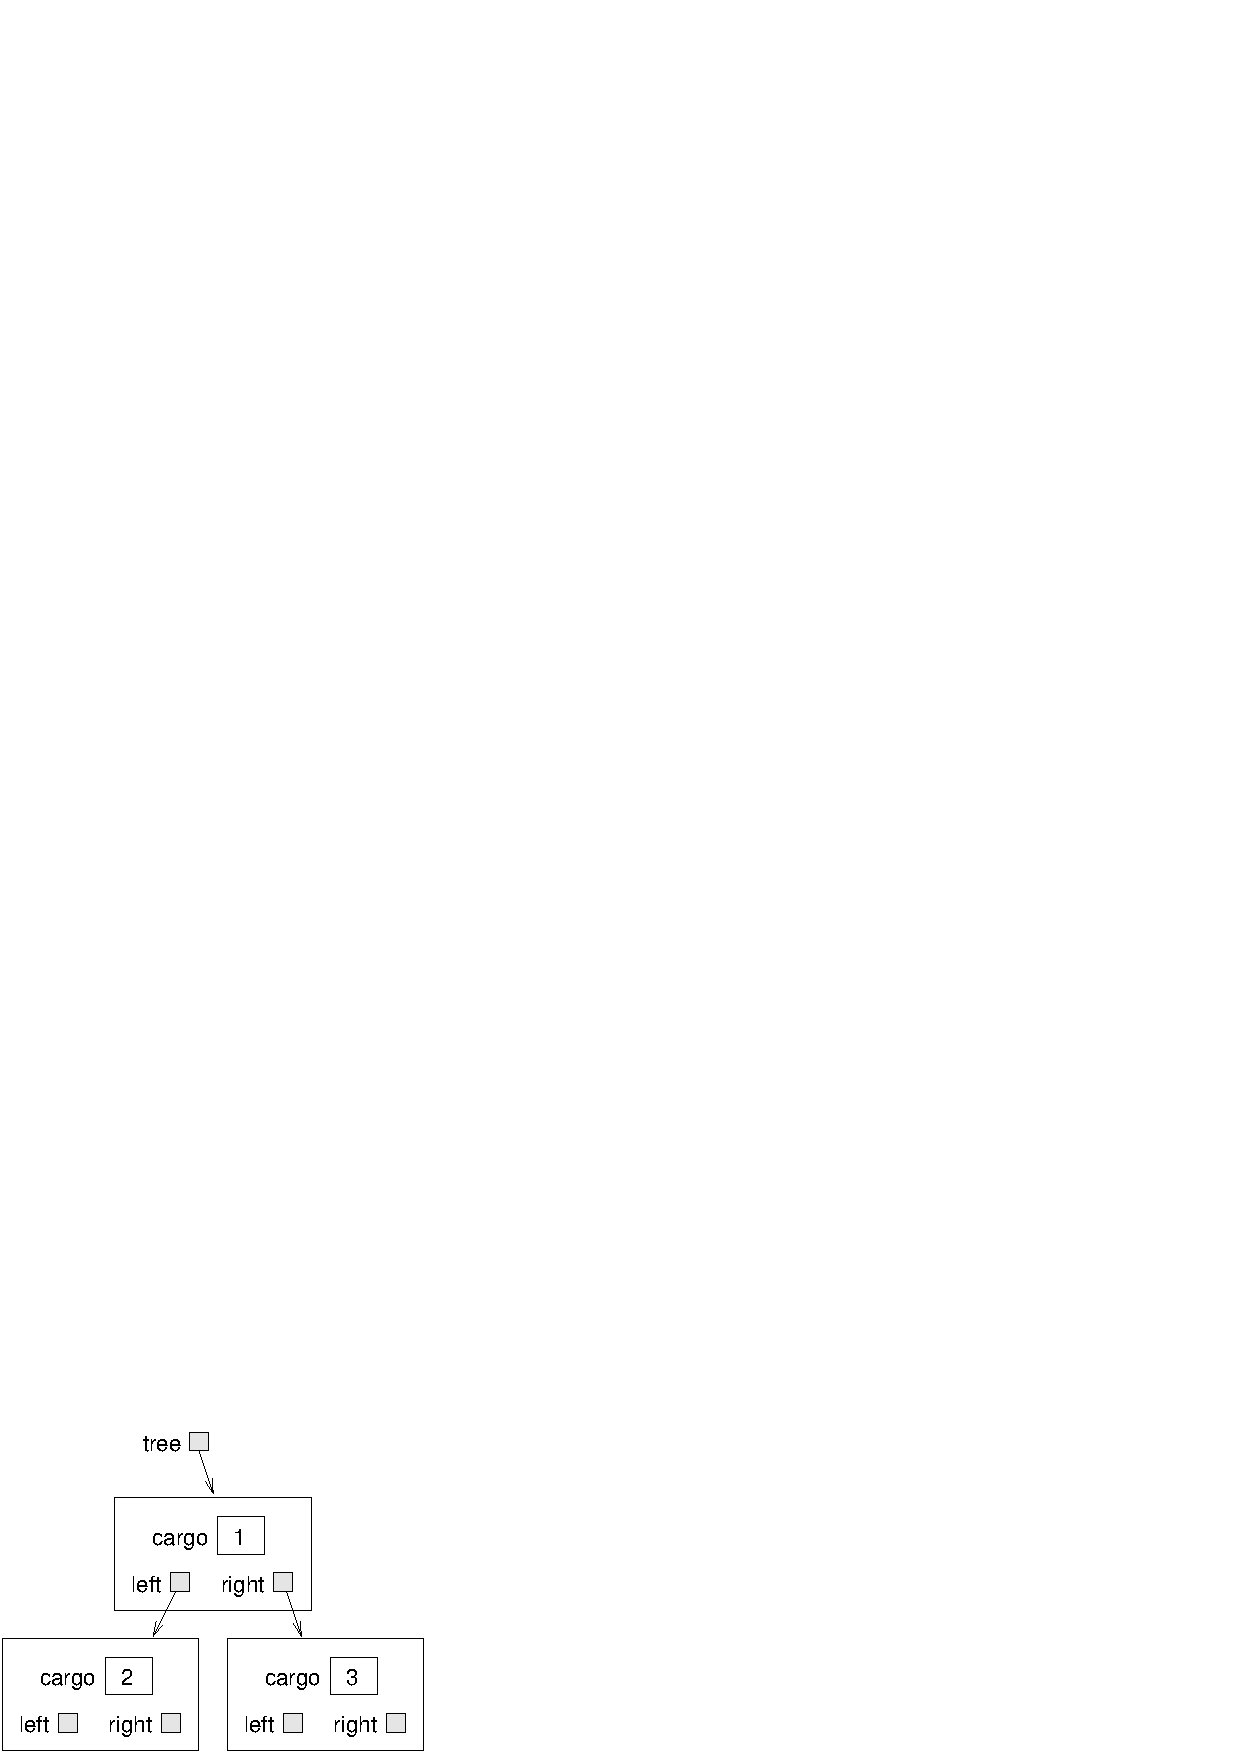
\includegraphics{figs/tree1.pdf}

The top of the tree (the node referred to by {\tt tree}) is
called the {\bf root}.  In keeping with the tree
metaphor, the other nodes are called branches and the nodes
at the tips with null references are called {\bf leaves}.  It
may seem odd that we draw the picture with the root at the top
and the leaves at the bottom, but that is not the strangest thing.

\index{root node}
\index{leaf node}
\index{parent node}
\index{child node}
\index{level}

To make things worse, computer scientists mix in yet another
metaphor: the family tree.  The top node is sometimes called
a {\bf parent} and the nodes it refers to are its {\bf children}.
Nodes with the same parent are called {\bf siblings}, and so on.

Finally, there is also a geometric vocabulary for taking
about trees.  I already mentioned left and right, but there is
also ``up'' (toward the parent/root) and down (toward the
children/leaves).  Also, all the nodes that are the same
distance from the root comprise a {\bf level} of the tree.

I don't know why we need three metaphors for talking about trees,
but there it is.


\section {Building trees}
\index{tree!linked implementation}

The process of assembling tree nodes is similar
to the process of assembling lists.
We have a constructor for tree nodes that initializes the instance
variables.

\begin{verbatim}
    public Tree (Object cargo, Tree left, Tree right) {
        this.cargo = cargo;
        this.left = left;
        this.right = right;
    }
\end{verbatim}
%
We allocate the child nodes first:

\begin{verbatim}
    Tree left = new Tree (new Integer(2), null, null);
    Tree right = new Tree (new Integer(3), null, null);
\end{verbatim}
%
We can create the parent node and link it to the children
at the same time:

\begin{verbatim}
    Tree tree = new Tree (new Integer(1), left, right);
\end{verbatim}
%
This code produces the state shown in the previous figure.


\section {Traversing trees}
\index{tree!traversal}
\index{traverse}

The most natural
way to traverse a tree is recursively.  For example, to
add up all the integers in a tree, we could write this class
method:

\begin{verbatim}
    public static int total (Tree tree) {
        if (tree == null) return 0;
        Integer cargo = (Integer) tree.cargo;
        return cargo.intValue() + total (tree.left) + total (tree.right);
    }
\end{verbatim}
%
This is a class method because we would like to use {\tt null} to
represent the empty tree, and make the empty tree the base case of the
recursion.  If the tree is empty, the method returns {\tt 0}.
Otherwise it makes two recursive calls to find the total value of its
two children.  Finally, it adds in its own cargo and returns the
total.

\index{tree!empty}

Although this method works, there is some difficulty fitting it into
an object-oriented design.
It should not appear in the {\tt Tree} class because it
requires the cargo to be {\tt Integer} objects.  If we make that
assumption in {\tt Tree.java} then we lose the advantages of a generic
data structure.

On the other hand, this code accesses the instance variables
of the {\tt Tree} nodes, so it ``knows'' more than it should about
the implementation of the tree.  If we change that implementation
later this code will break.

Later in this chapter we will develop ways to solve this problem,
allowing client code to traverse trees containing any kinds of objects
without breaking the abstraction barrier between the client code and
the implementation.  Before we get there, let's look at an
application of trees.


\section {Expression trees}
\index{tree!expression}
\index{expression tree}
\index{postfix}
\index{infix}

A tree is a natural way to represent the structure of a
mathematical expression.
Unlike other notations, it can represent the computation unambiguously.
For example, the infix expression {\tt 1 + 2 * 3} is ambiguous unless
we know that the multiplication happens before the addition.

The following figure represents the same computation:

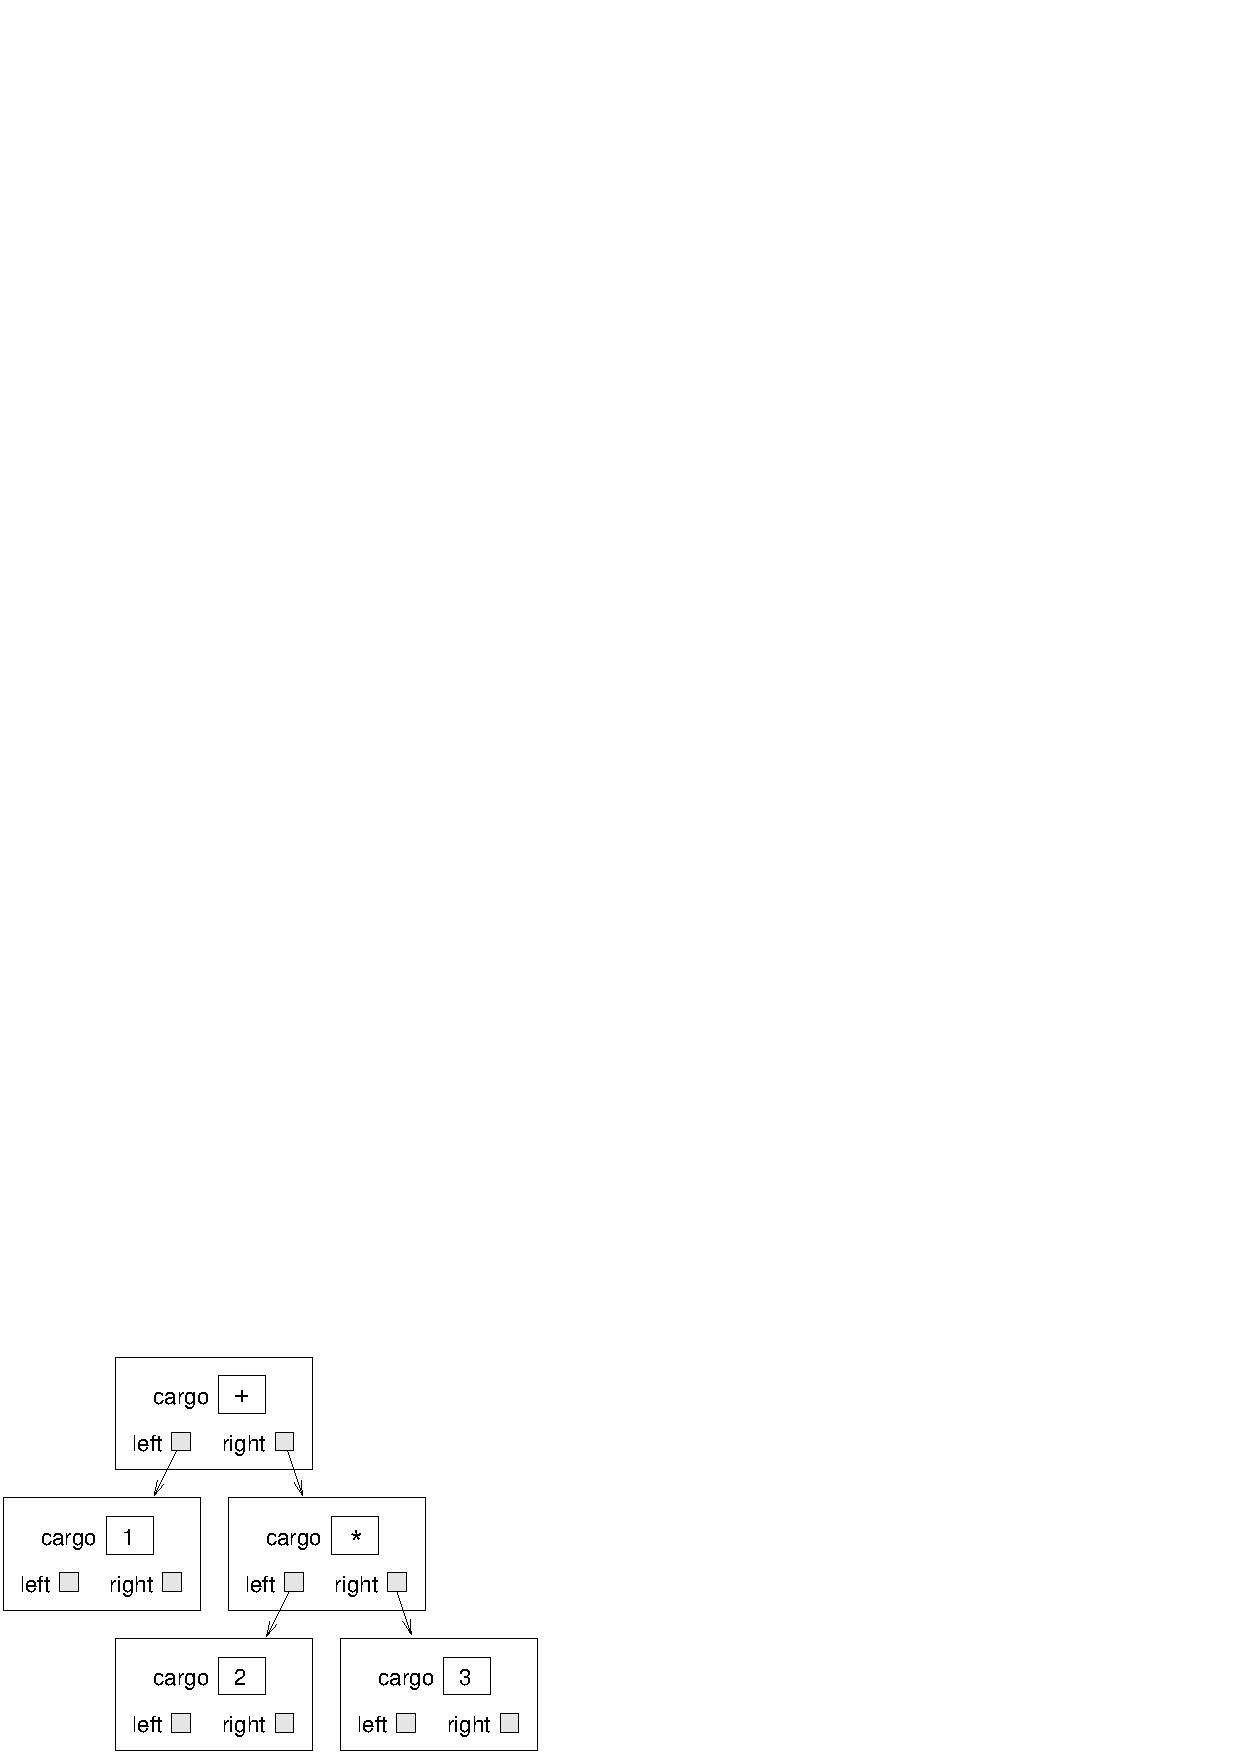
\includegraphics{figs/tree2.pdf}

The nodes can be operands like {\tt 1} and {\tt 2} or operators
like {\tt +} and {\tt *}.  Operands are leaf nodes; operator nodes 
contain references to their operands (all of these operators
are {\bf binary}, meaning they have exactly two operands).

Looking at this figure, there is no question what the order of
operations is: the multiplication happens first in order to compute
the first operand of the addition.

Expression trees like this have many uses.  The example we are
going to look at is translation from one format (postfix) to
another (infix).  Similar trees are used inside compilers to parse,
optimize and translate programs.


\section {Traversal}
\index{tree!traversal}
\index{traverse}
\index{recursion}
\index{preorder}
\index{postorder}
\index{inorder}

I already pointed out that recursion provides a natural way to
traverse a tree.  We can print the contents of an expression tree
like this:

\begin{verbatim}
    public static void print (Tree tree) {
        if (tree == null) return;
        System.out.print (tree + " ");
        print (tree.left);
        print (tree.right);
    }
\end{verbatim}
%
In other words, to print a tree, first print the contents of
the root, then print the entire left subtree, then print the
entire right subtree.  This way of traversing a tree is called
a {\bf preorder}, because the contents of the root appear before
the contents of the children.

For the example expression the output is {\tt + 1 * 2 3}.  This
is different from both postfix and infix; it is a new notation called
{\bf prefix}, in which the operators appear before their operands.

You might suspect that if we traverse the tree in a
different order we get the expression in a different
notation.  For example, if we print the subtrees first, and then
the root node:

\begin{verbatim}
    public static void printPostorder (Tree tree) {
        if (tree == null) return;
        printPostorder (tree.left);
        printPostorder (tree.right);
        System.out.print (tree + " ");
    }
\end{verbatim}
%
We get the expression in postfix ({\tt 1 2 3 * +})!  As the
name of the method implies, this order of traversal
is called {\bf postorder}.  Finally, to traverse a tree {\bf inorder},
we print the left tree, then the root, then the right tree:

\begin{verbatim}
    public static void printInorder (Tree tree) {
        if (tree == null) return;
        printInorder (tree.left);
        System.out.print (tree + " ");
        printInorder (tree.right);
    }
\end{verbatim}
%
The result is {\tt 1 + 2 * 3}, which is the expression in infix.

To be fair, I have to point out that I omitted an
important complication.  Sometimes when we write an expression
in infix we have to use parentheses to preserve the order of
operations.  So an inorder traversal is not quite sufficient to
generate an infix expression.

Nevertheless, with a few improvements, the expression tree 
and the three recursive traversals provide 
a general way to translate expressions from one format to
another.


\section {Encapsulation}
\index{encapsulation}
\index{client}
\index{provider}
\index{metaclass}

As I mentioned before, there is a problem with the way we have been
traversing trees: it breaks down the barrier between the client code
(the application that uses the tree) and the provider code (the Tree
implementation).  Ideally, tree code should be general; it shouldn't
know anything about expression trees.  And the code that generates and
traverses the expression tree shouldn't know about the implementation
of the trees.  This design criterion is called {\bf object
encapsulation} to distinguish it from the encapsulation we saw in
Section~\ref{encapsulation}, which we might call {\bf method
encapsulation}.

In the current version, the {\tt Tree} code knows too much about
the client.  Instead, the {\tt Tree} class should provide
the general capability of traversing a tree in various ways.  As
it traverses, it should perform operations on each node that are
specified by the client.


\index{Visitable}
\index{metaclass!Visitable}

To facilitate this separation of interests, we will
create a new metaclass, called {\tt Visitable}.  The items
stored in a tree will be required to be visitable, which means
that they define a method named {\tt visit} that does whatever
the client wants done to each node.  That way the
Tree can perform the traversal and the client can perform
the node operations.

Here are the steps we have to perform to wedge a metaclass
between a client and a provider:

\begin{enumerate}

\item Define a metaclass that specifies the methods
the provider code will need to invoke on its components.

\item Write the provider code in terms of the new metaclass,
as opposed to generic {\tt Objects}.

\item Define a class that belongs to the metaclass
and that implements the required methods 
as appropriate for the client.

\item Write the client code to use the new class.

\end{enumerate}

The next few sections demonstrate these steps.


\section {Defining a metaclass}
\index{metaclass!defining}
\index{interface}

There are actually two ways to implement a metaclass in Java,
an an {\bf interface} or as an {\bf abstract class}.  The differences
between them aren't important for now, so we'll start by
defining an interface.

An interface definition looks a lot like a class
definition, with two differences:

\begin{itemize}

\item The keyword {\tt class} is replaced with {\tt interface}, and

\item The method definitions have no bodies.

\end{itemize}

An interface definition specifies the methods a class has to
implement in order to be in the metaclass.  The specification
includes the name, parameter
types, and return type of each method.

The definition of {\tt Visitable} is

\begin{verbatim}
public interface Visitable {
    public void visit ();
}
\end{verbatim}
%
That's it!  The definition of {\tt visit} looks like any other
method definition, except that it has no body.  This definition
specifies that any class that implements {\tt Visitable} has to have
a method named {\tt visit} that takes no parameters and that returns
{\tt void}.

\index{body!method}

Like other class definitions, interface definitions go in a file
with the same name as the class (in this case {\tt Visitable.java}).


\section {Implementing a metaclass}
\index{metaclass!implementing}
\index{Token class}
\index{class!Token}

If we are using an expression tree to generate infix, then
``visiting'' a node means printing its contents.  Since the
contents of an expression tree are tokens, we'll create a new
class called {\tt Token} that implements {\tt Visitable}

\begin{verbatim}
public class Token implements Visitable {
    String str;

    public Token (String str) {
        this.str = str;
    }

    public void visit () {
        System.out.print (str + " ");
    }
}
\end{verbatim}
%
When we compile this class definition (which is in a file named {\tt
Token.java}), the compiler checks whether the methods provided satisfy
the requirements specified by the metaclass.  If not, it will
produce an error message.  For example, if we misspell the name of the
method that is supposed to be {\tt visit}, we might get
something like, ``class Token must be declared abstract. It does not
define void visit() from interface Visitable.''  This is one of
many error messages where the solution suggested by the compiler
is wrong.  When it says the class ``must be declared abstract,''
what it means is that you have to fix the class so that it implements
the interface properly.  Sometimes I think the people who write
these messages should be beaten.

The next step is to modify the parser to put {\tt Token} objects
into the tree instead of {\tt Strings}.  Here is a small example:

\begin{verbatim}
    String expr = "1 2 3 * +";
    StringTokenizer st = new StringTokenizer (expr, " +-*/", true);
    String token = st.nextToken();
    Tree tree = new Tree (new Token (token), null, null));
\end{verbatim}
%
This code takes the first token in the string and wraps it in
a {\tt Token} object, then puts the {\tt Token} into a tree node.
If the {\tt Tree} requires the cargo to be {\tt Visitable}, it
will convert the {\tt Token} to be a {\tt Visitable} object.
When we remove the {\tt Visitable} from the tree, we will have
to cast it back into a {\tt Token}.

\begin{exercise}
Write a version of {\tt printPreorder} called
{\tt visitPreorder} that traverses the tree and invokes
{\tt visit} on each node in preorder.
\end{exercise}

The flow of execution for methods like {\tt visitPreorder} is
unusual.  The client invokes a method provided by the Tree
implementation, and then the tree implementation invokes a
method provided by the client.  This pattern is called a
{\bf callback}; it is a good way to make provider code more
general without breaking down the abstraction barrier.

\index{callback}


\section {The {\tt Vector} class}
\label{vector}
\index{Vector class}
\index{class!Vector}

The {\tt Vector} is a built-in Java class in the {\tt java.util}
package.  It is an implementation of an array of {\tt Objects},
with the added feature that it can resize itself automatically,
so we don't have to.

Before using the {\tt Vector} class, you should understand
a few concepts.  Every {\tt Vector} has a
capacity, which is the amount of space that has been allocated
to store values, and a size, which is the number of values that
are actually in the vector.

The following figure is a simple diagram of a {\tt Vector}
that contains three elements, but it has a capacity of seven.

\includegraphics{figs/vector.pdf}

There are two sets of methods for accessing the elements of
a vector.  They provide different semantics and different
error-checking capabilities, and they are easy to get confused.

The simpler accessors methods are {\tt get} and {\tt set}, which
provide semantics similar to the array index operator {\tt []}.
{\tt get} takes an integer index and returns the element at the
indicated position.  {\tt set} takes an index and an element,
and stores the new element at the indicated position, replacing
the existing element.

{\tt get} and {\tt set} do not change the size of the vector (number
of elements).  It is the responsibility of the client code to make
sure that the vector has sufficient size before invoking {\tt set} or
{\tt get}.  The {\tt size} method returns the number of elements in
the Vector.  If you try to access an element that does not exist (in
this case the elements with indices 3 through 6), you will get an {\tt
ArrayIndexOutOfBounds} exception.

\index{exception!ArrayIndexOutOfBounds}
\index{ArrayIndexOutOfBounds}

The other set of methods includes several versions
of {\tt add} and {\tt remove}.  These methods change the size
of the Vector and, if necessary, the capacity.  One version
of {\tt add} takes an element as a parameter and adds it to the
end of the Vector.  This method is safe in the sense that it
will not cause an exception.

Another version of {\tt add}
takes an index and an element and, like {\tt set}, it puts
the new element at the given position.  The difference is
that {\tt add} doesn't replace the existing element; it
increases the size of the Vector and shifts elements to the
right to make room for the new one.  Thus, the invocation
{\tt v.add (0, elt)} add the new element at the beginning
of the Vector.  Unfortunately, this method is neither
safe nor efficient; it can cause an {\tt ArrayIndexOutOfBounds}
exception and, in most implementations, it is linear time
(proportional to the size of the Vector).

Most of the time the client doesn't have to worry about
capacity.  Whenever the size of the {\tt Vector} changes,
the capacity is updated automatically.
For performance reasons, some applications take
control of this function, which is why there are additional methods
for increasing and decreasing capacity.

Because the client code has no access to the implementation of
a vector, it is not clear how we should traverse one.  Of course,
one possibility is to use a loop variable as an index into the
vector:

\begin{verbatim}
        for (int i=0; i<v.size(); i++) {
            System.out.println (v.get(i));
        }
\end{verbatim}
%
There's nothing wrong with that, but there is another way that
serves to demonstrate the {\tt Iterator} class.  Vectors provide
a method named {\tt iterator} that returns an {\tt Iterator} object
that makes it possible to traverse the vector.


\section {The {\tt Iterator} class}
\label{iterator}
\index{Iterator class}
\index{class!Iterator}
\index{metaclass}

{\tt Iterator} is an interface in the {\tt java.util}
package.  It specifies three methods:

\begin{description}

\item [{\tt hasNext}:] Does this iteration have more elements?

\item [{\tt next}:] Return the next element, or throw an exception if
there is none.

\item [{\tt remove}:] Remove the most recent
element from the data structure we are traversing.

\end{description}

The following example uses an iterator to traverse and print the
elements of a vector.

\begin{verbatim}
        Iterator it = vector.iterator ();
        while (it.hasNext ()) {
            System.out.println (it.next ());
        }
\end{verbatim}
%
Once the {\tt Iterator} is created, it is a separate object from
the original {\tt Vector}.  Subsequent changes in the {\tt Vector}
are not reflected in the {\tt Iterator}.  In fact, if you
modify the {\tt Vector} after creating an {\tt Iterator},
the {\tt Iterator} becomes invalid.  If you access the
{\tt Iterator} again, it will cause a {\tt ConcurrentModification}
exception.

\index{exception!ConcurrentModification}
\index{ConcurrentModification}

In a previous section we used the {\tt Visitable} metaclass to
allow a client to traverse a data structure without knowing the
details of its implementation.  Iterators provide another way to do
the same thing.  In the first case, the provider performs the iteration
and invokes client code to ``visit'' each element.  In the second
case the provider gives the client an object that it can use to
select elements one at a time (albeit in an order controlled by
the provider).

\begin{exercise}
Write a class named {\tt PreIterator} that
implements the {\tt Iterator} interface, and write a method named {\tt
preorderIterator} for the {\tt Tree} class that returns a {\tt
PreIterator} that selects the elements of the {\tt Tree} in preorder.

HINT: The easiest way to build an Iterator is to put elements
into a Vector in the order you want and then invoke {\tt iterator}
on the Vector.
\end{exercise}


\section{Glossary}
\index{binary tree}
\index{root node}
\index{leaf node}
\index{parent node}
\index{child node}
\index{level}
\index{prefix}
\index{preorder}
\index{postorder}
\index{inorder}
\index{class variable}
\index{encapsulation}
\index{callback}

\begin{description}

\item[binary tree:]  A tree in which each node refers to 0, 1, or
2 dependent nodes.

\item[root:]  The top-most node in a tree, to which no other nodes
refer.

\item[leaf:]  A bottom-most node in a tree, which refers to no other
nodes.

\item[parent:]  The node that refers to a given node.

\item[child:]  One of the nodes referred to by a node.

\item[level:]  A set of nodes equidistant from the root.

\item[prefix notation:]  A way of writing a mathematical expression
with each operator appearing before its operands.

\item[preorder:]  A way to traverse a tree, visiting each node
before its children.

\item[postorder:]  A way to traverse a tree, visiting the children
of each node before the node itself.

\item[inorder:]  A way to traverse a tree, visiting the left subtree,
then the root, then the right subtree.

\item[class variable:]  A {\tt static} variable declared outside of any
method.  It is accessible from any method.

\item[binary operator:]  An operator that takes two operands.

\item[object encapsulation:]  The design goal of keeping
the implementations of two objects as separate as possible.  Neither
class should have to know the details of the implementation of
the other.

\item[method encapsulation:]  The design goal of keeping the
interface of a method separate from the details of its implementation.

\item[callback:] A flow of execution where provider code invokes
a method provided by the client.

\end{description}


\section{Exercises}

\begin{exercise}
\begin{enumerate}

\item What is the value of the postfix expression 
{\tt 1 2 + 3 *}?

\item What is the postfix expression that is equivalent to
the infix expression {\tt 1 + 2 * 3}?

\item What is the value of the postfix expression 
{\tt 17 1 - 5 /}, assuming that {\tt /} performs integer division? 

\end{enumerate}
\end{exercise}


\begin{exercise}
\label{ex.height}
The height of a tree is the longest path from the root to
any leaf.  Height can be defined recursively as follows:

\begin{itemize}

\item The height of a null tree is 0.

\item The height of a non-null tree is {\tt 1 + max (leftHeight, rightHeight)},
where {\tt leftHeight} is the height of the left child and {\tt rightHeight}
is the height of the right child.

\end{itemize}

Write a method named {\tt height} that calculates the height of
the {\tt Tree} provided as a parameter.
\end{exercise}


\begin{exercise}
Imagine we define a Tree that contains Comparable objects as
cargo:

\begin{verbatim}
public class ComparableTree {
    Comparable cargo;
    Tree left, right;
}
\end{verbatim}

Write a {\tt Tree} class method named {\tt findMax}
that returns the largest cargo in
the tree, where ``largest'' is defined by {\tt compareTo}.
\end{exercise}


\begin{exercise}
\label{ex.searchtree}
\index{tree!search}
\index{search tree}
\index{binary search tree}
A binary search tree is a special kind of tree where,
for every node N:

\vspace{0.1in}
all the cargo in the left subtree of N $<$ the cargo in node N

and

the cargo in node N $<$ all the cargo in the right subtree of N
\vspace{0.1in}

Using the following class definition, write an object method called
{\tt contains} that takes an {\tt Object} as an argument and that
returns true if the object appears in the tree or false otherwise.
You can assume that the target object and all the objects in the
tree are {\tt Comparable}.

\begin{verbatim}
public class SearchTree {
    Comparable cargo;
    SearchTree left, right;
}
\end{verbatim}
\end{exercise}


\begin{exercise}
\label{ex.treeset}
In mathematics, a {\bf set} is a collection of elements that
contains no duplicates.
The interface {\tt java.util.Set} is intended to model a mathematical
set.  The methods it requires are {\tt add}, {\tt contains},
{\tt containsAll}, {\tt remove}, {\tt size}, and {\tt iterator}.

Write a class called {\tt TreeSet} that extends {\tt SearchTree}
and that implements {\tt Set}.  
To keep things simple, you can assume that {\tt null} does
not appear in the tree or as an argument to any of the methods.
\end{exercise}


\begin{exercise}
Write a method called {\tt union} that takes two Sets as
parameters and returns a new {\tt TreeSet} that contains all
the elements that appear in either Set.

You can add this method to your implementation of {\tt TreeSet},
or create a new class that extends {\tt java.util.TreeSet} and
provides {\tt union}.
\end{exercise}

\begin{exercise}
Write a method called {\tt intersection} that takes two Sets as
parameters and returns a new {\tt TreeSet} that contains all
the elements that appear in both Sets.

{\tt union} and {\tt intersection} are generic in the sense that
the parameters can be any type in the metaclass {\tt Set}.  The
two parameters don't even have to be the same type.
\end{exercise}


\begin{exercise}
One of the reasons the {\tt Comparable} interface is useful is
that it allows an object type to specify whatever ordering is
appropriate.
For types like {\tt Integer} and {\tt Double}, the
appropriate 
ordering is obvious, but there are lots of examples where the
ordering depends on what the objects are supposed
to represent.  In golf, for example, a low score is better than
a high score; if we compare two {\tt Golfer} objects,
the one with the lower score wins.

\begin{enumerate}

\item Write a definition of a Golfer class that contains a
name and an integer score as instance variables.  The class
should implement {\tt Comparable} and provide a {\tt compareTo}
method that gives higher priority to the lower score.

\item Write a program that reads a file containing the names
and scores of a set of golfers.  It should create Golfer objects,
put them in a Priority Queue and then take them out and print them.
They should appear in descending order of priority, which is
increasing order by score.

\begin{verbatim}
        Tiger Woods     61
        Hal Sutton      69
        Phil Mickelson  72
        Allen Downey   158
\end{verbatim}

\end{enumerate}

HINT: See Section~\ref{fileIO} for code that reads lines
from a file.
\end {exercise}


\begin{exercise}
Write an implementation of a Stack using a Vector.  Think about
whether it is better to push new elements onto the beginning or
the end of the Vector.
\end{exercise}





\chapter{Heaps}

\section{Array implementation of a tree}
\index{tree!array implementation}
\index{implementation!Tree}
\index{ADT!Tree}

What does it mean to ``implement'' a tree?  So far we have only seen
one implementation of a tree, a linked data structure similar to a
linked list.  But there are other structures we would like to identify
as trees.  Anything that can perform the basic set of tree operations
should be recognized as a tree.

So what are the tree operations?  In other words, how do we define
the Tree ADT?

\begin{description}

\item[constructor:]  Build an empty tree.

\item[{\tt getLeft}:]  Return the left child of this node.

\item[{\tt getRight}:]  Return the left child of this node.

\item[{\tt getParent}:]  Return the parent of this node.

\item[{\tt getCargo}:]  Return the cargo object from this node.

\item[{\tt setCargo}:]  Assign a cargo object to this node
(and create the node, if necessary).

\end{description}

In the linked implementation, the empty tree is represented by the
special value {\tt null}.  {\tt getLeft} and {\tt getRight} are
performed by accessing the instance variables of the node, as are {\tt
getCargo} and {\tt setCargo}.  We have not implemented {\tt getParent}
yet (you might think about how to do it).

There is another implementation of trees that uses arrays and
indices instead of objects and references.  To see how it works,
we will start by looking at a hybrid implementation that uses
both arrays and objects.

This figure shows a tree like the ones we have been looking at,
although it is laid out at an angle.
At the right there is an array of
references that refer to the cargo in the nodes.

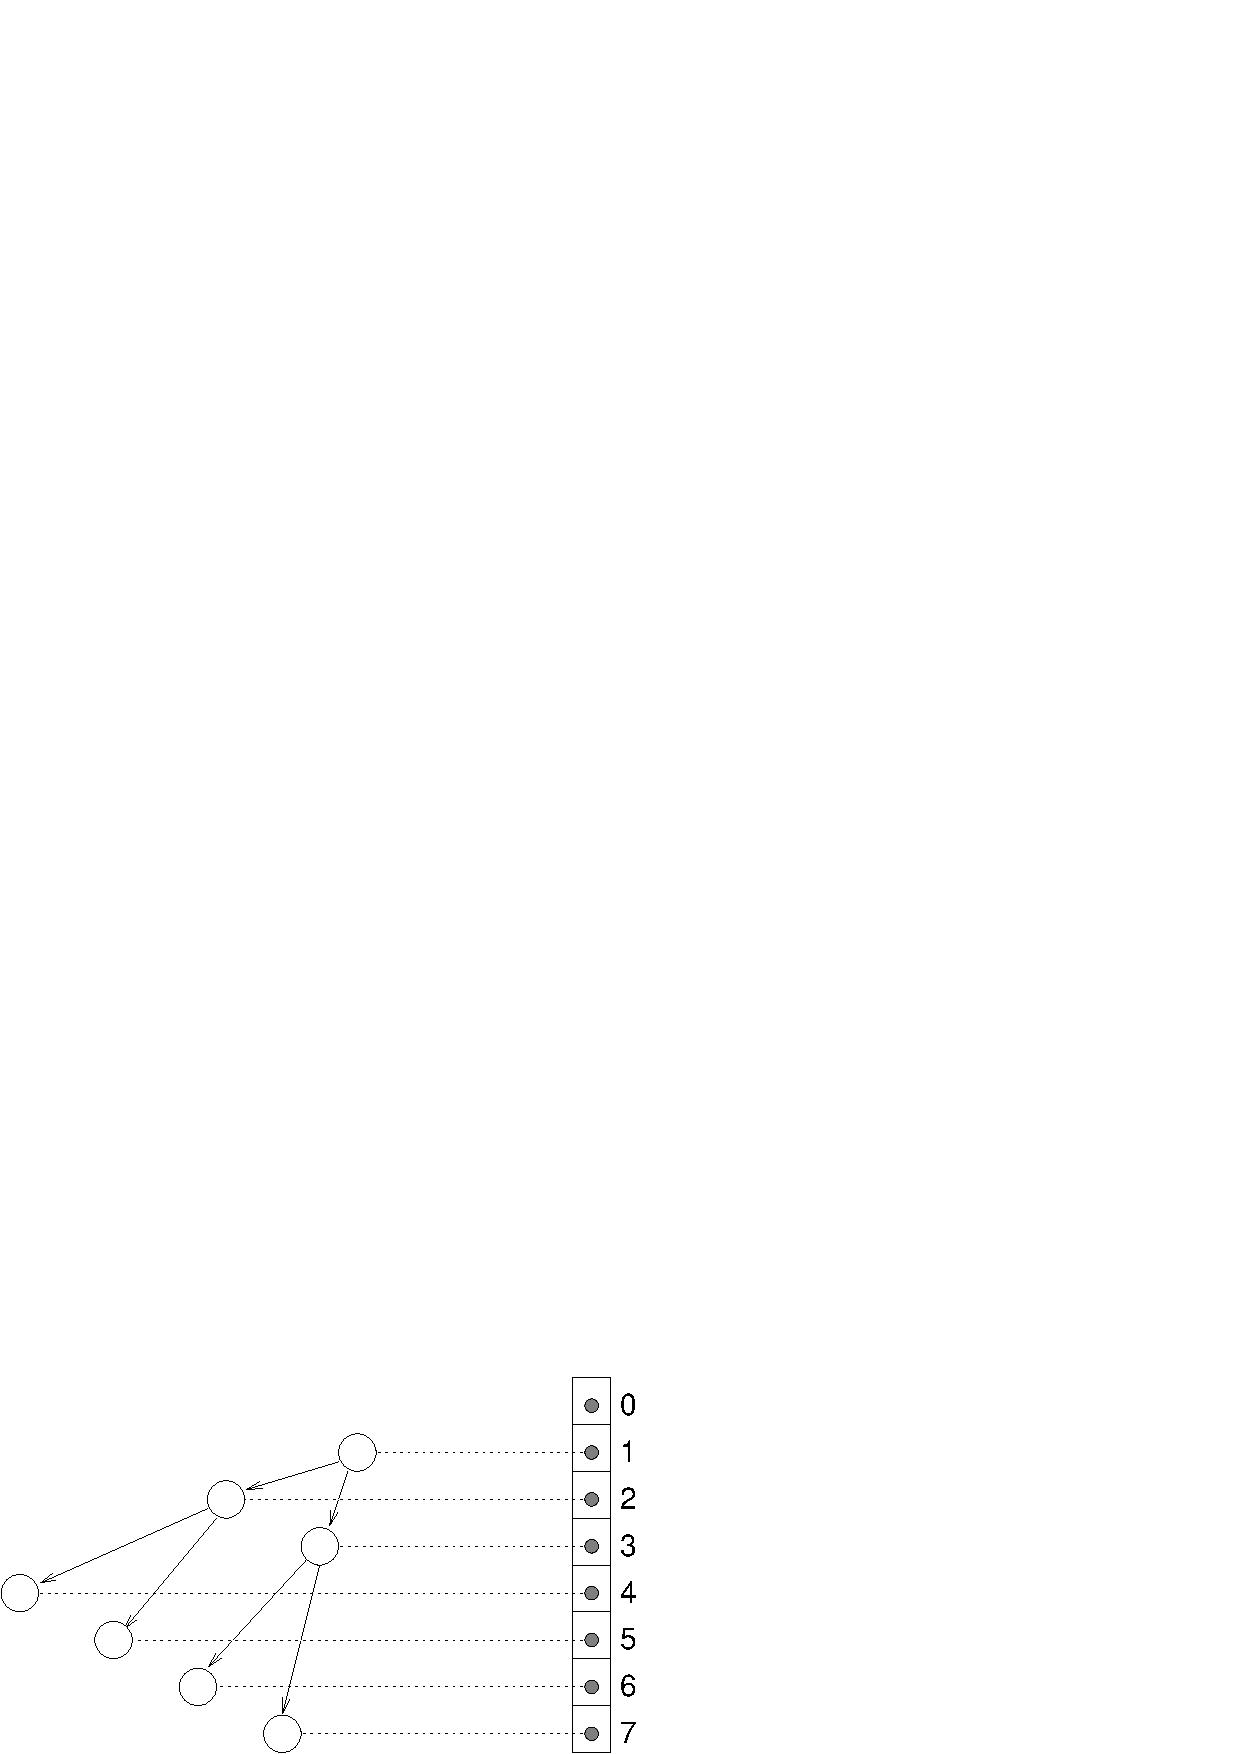
\includegraphics{figs/tree3.pdf}

Each node in the tree has a unique index.
Furthermore, the indices have been assigned to the nodes according
to a deliberate pattern, in order to achieve the following
results:

\begin{enumerate}

\item The left child of the node with index $i$ has index $2i$.

\item The right child of the node with index $i$ has index $2i + 1$.

\item The parent of the node with index $i$ has index $i/2$ (rounded down).

\end{enumerate}

Using these formulas, we can implement {\tt getLeft}, {\tt getRight}
and {\tt getParent} just by doing arithmetic; we don't have to
use the references at all!

Since we don't use the references, we can get rid of them,
which means that what used to be a tree node is now just cargo
and nothing else.  That means we can implement the tree as an
array of cargo objects; we don't need tree nodes.

Here's what one implementation looks like:

\begin{verbatim}
public class ArrayTree {
    Object[] array;
    int size;

    public ArrayTree () {
        array = new Object [128];
    }
\end{verbatim}
%
No surprises so far.  The only instance variable is
the array of {\tt Objects} that contains the tree's cargo.
The constructor initializes the array
with an arbitrary initial capacity; the result is an empty tree.

Here is the simplest implementation of {\tt getCargo}
and {\tt setCargo}.

\begin{verbatim}
    public Object getCargo (int i) {
        return array[i];
    }

    public void setCargo (int i, Object obj) {
        array[i] = obj;
    }
\end{verbatim}

These methods don't do any error-checking, so if the parameter is
wrong, they might generate an {\tt ArrayIndexOutOfBounds}
exception.

The implementation of {\tt getLeft}, {\tt getRight}
and {\tt getParent} is just arithmetic:

\begin{verbatim}
    public int getLeft (int i)  { return 2*i; }
    public int getRight (int i) { return 2*i + 1; }
    public int parent (int i)   { return i/2; }
\end{verbatim}
%
Finally we are ready to build a tree.  In another class (the client),
we would write

\begin{verbatim}
    ArrayTree tree = new ArrayTree ();
    tree.setCargo (1, "cargo for root");
\end{verbatim}
%
The constructor builds an empty tree.
Invoking {\tt setCargo} puts the
string {\tt "cargo for root"} into the root node.

To add children to the root nodes:

\begin{verbatim}
    tree.setCargo (tree.getLeft(1), "cargo for left");
    tree.setCargo (tree.getRight(1), "cargo for right");
\end{verbatim}
%
In the tree class we could provide a method that prints
the contents of the tree in preorder.

\begin{verbatim}
    public void print (int i) {
        Object cargo = tree.getCargo (i);
        if (cargo == null) return;
        System.out.println (cargo);
        print (getRight (i));
        print (getLeft (i));
    }
\end{verbatim}
%
To invoke this method, we have to pass the index of
the root as a parameter.

\begin{verbatim}
    tree.print (1);
\end{verbatim}
%
The output is

\begin{verbatim}
cargo for root
cargo for left
cargo for right
\end{verbatim}
%
This implementation provides the basic operations that define a
tree.  As I pointed out, the linked implementation of a tree provides
the same operations, but the syntax is different.

In some ways, the array implementation is a bit awkward.  For
one thing, we assume that {\tt null} cargo indicates a non-existent
node, but that means that we can't put a {\tt null} object in the
tree as cargo.

Another problem is that subtrees aren't represented as objects;
they are represented by indices into the array.  To pass a tree
node as a parameter, we have to pass a reference to the tree
object and an index into the array.
Finally, some operations that are easy in the linked implementation,
like replacing an entire subtree, are harder in the array implementation.

On the other hand, this implementation saves space, since there are
no links between the nodes, and
there are several operations that are easier and faster
in the array implementation.  It turns out that these operations
are just the ones we want to implement a Heap.

A Heap is an implementation of the Priority Queue
ADT that is based on the array implementation of a Tree.  It
turns out to be more efficient than the other implementations
we have seen.

To prove this claim, we will proceed in a few steps.
First, we need to develop ways of comparing the performance of
various implementations.  Next, we will look at the operations
Heaps perform.  Finally, we will compare the Heap implementation
of a Priority Queue to the others (arrays and lists) and see
why the Heap is considered particularly efficient.


\section {Performance analysis}
\index{performance analysis}
\index{run time}
\index{algorithm analysis}

When we compare algorithms, we would like to have a way to tell
when one is faster than another, or takes less space, or uses less
of some other resource.  It is hard to answer those questions in
detail, because the time and space used by an algorithm depend on the
implementation of the algorithm, the particular problem being
solved, and the hardware the program runs on.

The objective of this section is to develop a way of talking about
performance that is independent of all of those things, and only
depends on the algorithm itself.  To start, we will focus on run
time; later we will talk about other resources.

Our decisions are guided by a series of constraints:

\begin{enumerate}

\item First, the performance of an algorithm depends on the
hardware it runs on, so we usually don't talk about run time
in absolute terms like seconds.  Instead, we usually
count the number of abstract operations the algorithm performs.

\item Second, performance often depends on the particular
problem we are trying to solve -- some problems are easier than
others.  To compare algorithms, we usually focus on either the
worst-case scenario or an average (or common) case.

\item Third, performance depends on the size of the problem
(usually, but not always, the number of elements in a collection).
We address this dependence explicitly by
expressing run time as a function of problem size.

\item Finally, performance depends on
details of the implementation like object allocation overhead
and method invocation overhead.  We usually ignore these details
because they don't affect the rate at which the
number of abstract operations increases with problem size.

\end{enumerate}

To make this process more concrete, consider two algorithms we
have already seen for sorting an array of integers.  The
first is {\bf selection sort}, which we saw in Section~\ref{sorting}.
Here is the pseudocode we used there.

\begin{verbatim}
    selectionsort (array) {
        for (int i=0; i<array.length; i++) {
          // find the lowest item at or to the right of i
          // swap the ith item and the lowest item
        }
    }
\end{verbatim}
%
To perform the
operations specified in the pseudocode, we wrote helper methods named
{\tt findLowest} and {\tt swap}.  In pseudocode,
{\tt findLowest} looks like this

\begin{verbatim}
    // find the index of the lowest item between
    // i and the end of the array

    findLowest (array, i) {
        // lowest contains the index of the lowest item so far
        lowest = i;
        for (int j=i+1; j<array.length; j++) {
          // compare the jth item to the lowest item so far
          // if the jth item is lower, replace lowest with j
        }
        return lowest;
    }
\end{verbatim}
%
And {\tt swap} looks like this:

\begin{verbatim}
    swap (i, j) {
        // store a reference to the ith card in temp
        // make the ith element of the array refer to the jth card
        // make the jth element of the array refer to temp
    }
\end{verbatim}
%
To analyze the performance of this algorithm, 
the first step is to decide what operations to count.  Obviously,
the program does a lot of things: it increments {\tt i}, compares
it to the length of the deck, it searches for the largest element
of the array, etc.  It is not obvious what the right thing is
to count.

\index{sorting}
\index{selection sort}

It turns out that a good choice is the number of
times we compare two items.  Many other choices would yield
the same result in the end, but this is easy to do and we will
find that it allows us to compare the sorting algorithms
most easily.

The next step is to define the ``problem size.''  In this case
it is natural to choose the size of the array, which we'll call
$n$.

Finally, we would like to derive an expression that tells us how
many abstract operations (in this case, comparisons) we have to
do, as a function of $n$.

\index{helper method}

We start by analyzing the helper methods.  {\tt swap} copies several
references, but it doesn't perform any comparisons, so we ignore the
time spent performing swaps.  {\tt findLowest} starts at {\tt i} and
traverses the array, comparing each item to {\tt lowest}.  The number
of items we look at is $n-i$, so the total number of comparisons is
$n-i-1$.

Next we consider how many times {\tt findLowest}
gets invoked and what the value of $i$ is each time.  The last
time it is invoked, $i$ is $n-2$ so the number of
comparisons is 1.  The previous iteration performs 2 comparisons,
and so on.  During the first iteration, $i$ is $0$ and the
number of comparisons is $n-1$.

So the total number of comparisons is $1 + 2 + \cdots + n-1$.
This sum is equal to $n^2/2 - n/2$.  To describe this algorithm,
we would typically ignore the lower order term ($n/2$) and say
that the total amount of work is proportional to $n^2$.  Since
the leading order term is quadratic, we might also say that this
algorithm is {\bf quadratic time}.

\index{quadratic time}


\section {Analysis of mergesort}
\index{mergesort}
\index{analysis!mergesort}
\index{sorting}
\index{algorithm analysis}

In Section~\ref{mergesort} I claimed that mergesort takes time
that is proportional to $n \log n$, but I didn't explain how
or why.  Now I will.

Again, we start by looking at pseudocode for the algorithm.
For mergesort, it's

\begin{verbatim}
  mergeSort (array) {
    // find the midpoint of the array
    // divide the array into two halves
    // sort the halves recursively
    // merge the two halves and return the result
  }
\end{verbatim}
%
At each level of the recursion, we split the array in half,
make two recursive calls, and then merge the halves.  Graphically,
the process looks like this:
 
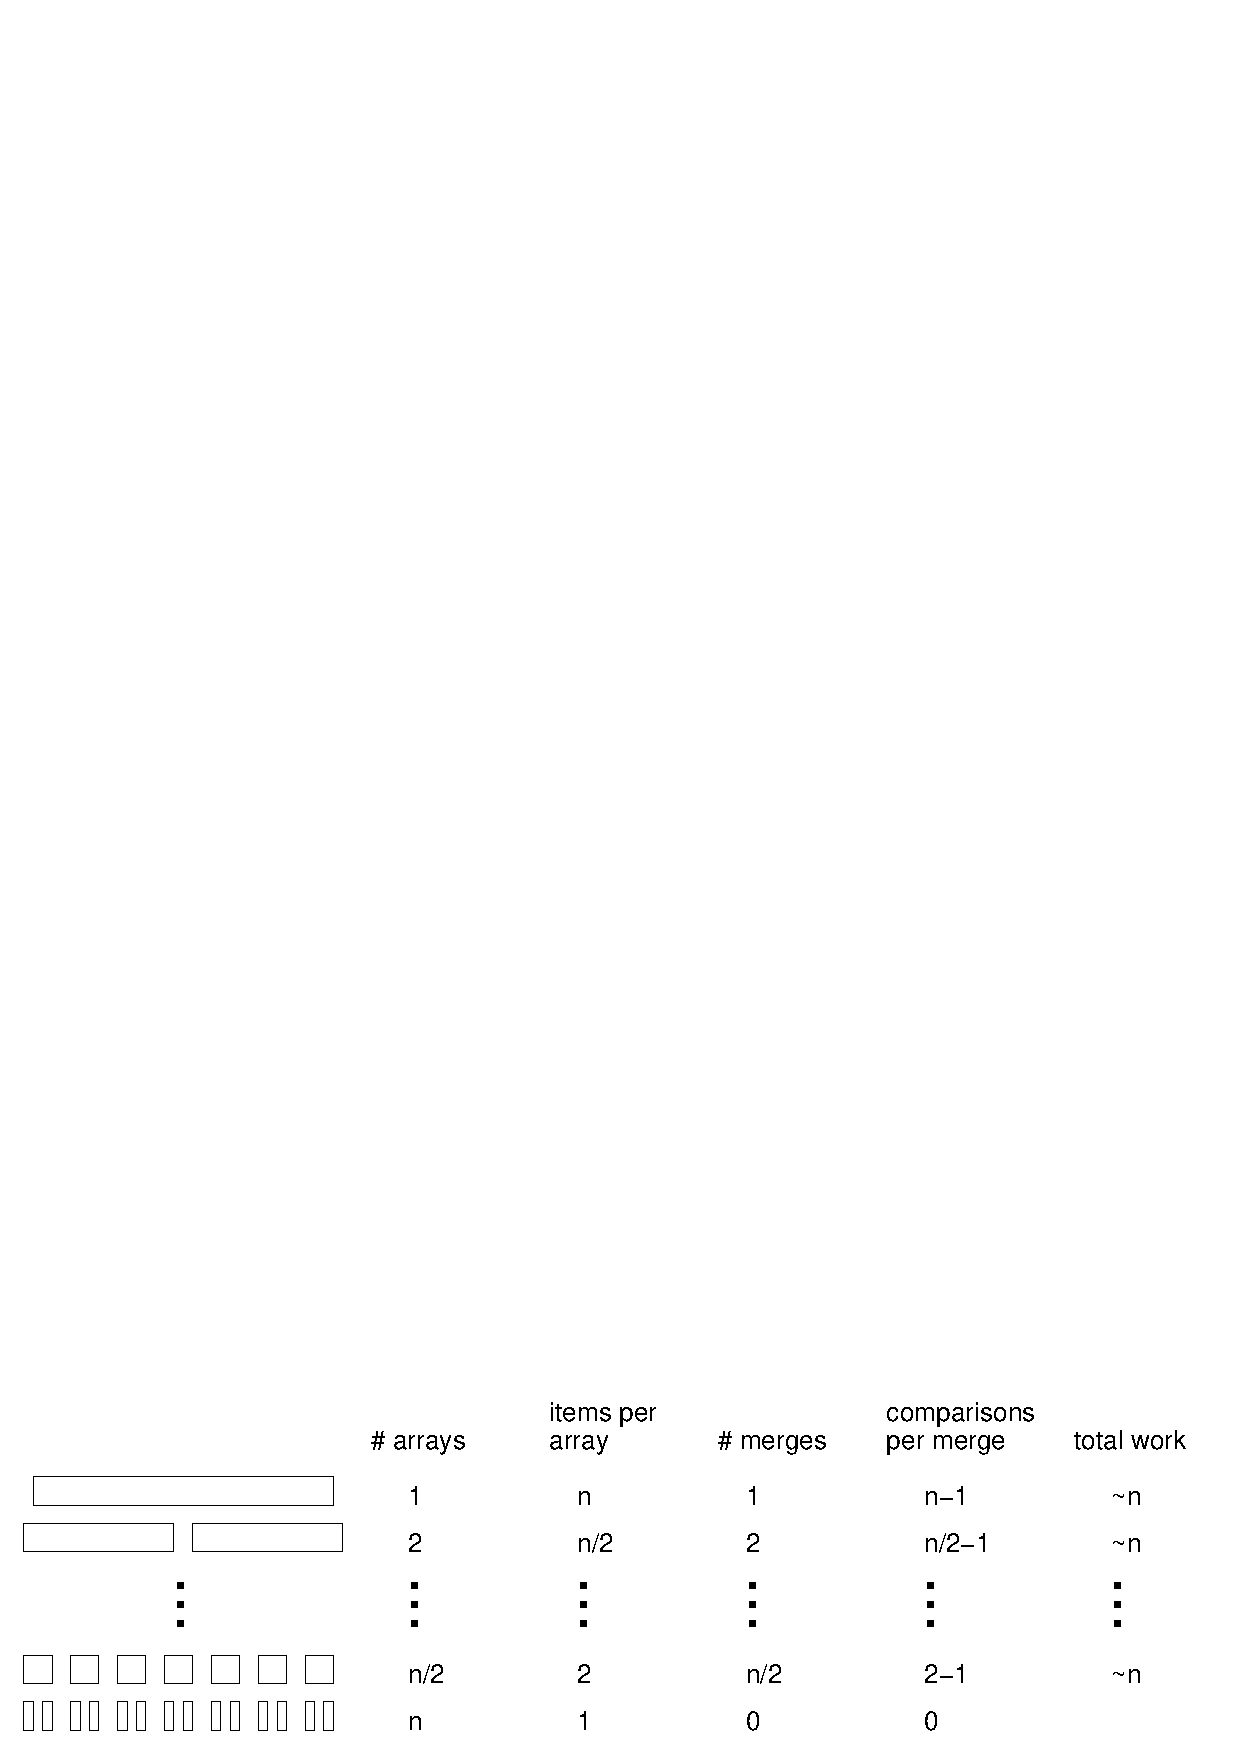
\includegraphics[width=5in]{figs/mergetree.pdf}
 
Each line in the diagram is a level of the recursion.  At the
top, a single array divides into two halves.  At the bottom, $n$
arrays with one element each are merged into $n/2$ arrays with
2 elements each.

\index{recursion}

The first two columns of the table show the number of arrays at each
level and the number of items in each array.  The third column shows
the number of merges that take place at each level of recursion.  The
next column is the one that takes the most thought: it shows the
number of comparisons each merge performs.

\index{pseudocode}

If you look at the pseudocode (or your implementation) of
merge, you should convince yourself that in the worst case it
takes $m-1$ comparisons, where $m$ is the total number items
being merged.

The next step is to multiply the number of merges at each level
by the amount of work (comparisons) per merge.  The result is the
total work at each level.  At this point we take advantage of a small
trick.  We know that in the end we are only interested in the
leading-order term in the result, so we can go ahead
and ignore the $-1$ term in the comparisons per merge.  If we do
that, then the total work at each level is simply $n$.

Next we need to know the number of levels as a function of $n$.  Well,
we start with an array of $n$ items and divide it in half until it
gets to 1.  That's the same as starting at 1 and multiplying by 2
until we get to $n$.  In other words, we want to know how many times
we have to multiply 2 by itself before we get to $n$.  The answer is
that the number of levels, $l$, is the logarithm, base 2, of $n$.

Finally, we multiply the amount of work per level, $n$, by the
number of levels, $\log_2 n$ to get $n \log_2 n$, as promised.
There isn't a good name for this functional form; most of the
time people just say, ``en log en.''

It might not be obvious at first that $n \log_2 n$ is better than
$n^2$, but for large values of $n$, it is.
As an exercise, write a program that prints $n \log_2 n$ and
$n^2$ for a range of values of $n$.


\section{Overhead}
\index{overhead}

Performance analysis takes a lot of handwaving.  First we ignored most
of the operations the program performs and counted only comparisons.
Then we decided to consider only worst case performance.  During the
analysis we took the liberty of rounding a few things off, and when we
finished, we casually discarded the lower-order terms.

When we interpret the results of this analysis, we have to keep
all this hand-waving in mind.  Because mergesort is $n \log_2 n$,
we consider it a better algorithm than selection sort, but that
doesn't mean that mergesort is {\em always} faster.  It just means
that eventually, if we sort bigger and bigger arrays, mergesort
will win.

How long that takes depends on the details of the implementation,
including the additional work, besides the comparisons we counted,
that each algorithm performs.  This extra work is sometimes called
{\bf overhead}.  It doesn't affect the performance analysis, but
it does affect the run time of the algorithm.

For example, our implementation of mergesort actually allocates
subarrays before making the recursive calls and then lets them get
garbage collected after they are merged.  Looking again at the diagram
of mergesort, we can see that the total amount of space that gets
allocated is proportional to $n \log_2 n$, and the total number of
objects that get allocated is about $2n$.  All that allocating takes
time.

Even so, it is most often true that a bad implementation of a good
algorithm is better than a good implementation of a bad algorithm.
The reason is that for large values of $n$ the good algorithm is
better and for small values of $n$ it doesn't matter because both
algorithms are good enough.

As an exercise, write a program that prints values of $1000 n \log_2
n$ and $n^2$ for a range of values of $n$.  For what value of $n$ are
they equal?


\section{Priority Queue implementations}
\index{implementation!Priority Queue}
\index{analysis!Priority Queue}
\index{priority queue!sorted list implementation}

In Chapter~\ref{queue} we looked at an implementation of a Priority
Queue based on an array.  The items in the array are unsorted, so it
is easy to add a new item (at the end), but harder to remove an
item, because we have to search for the item with the highest
priority.

An alternative is an implementation based on a sorted list.
In this case when we add a new item we traverse the list and
put the new item in the right spot.  This implementation takes
advantage of a property of lists, which is that it is easy to
add a new node into the middle.  Similarly, removing the
item with the highest priority is easy, provided that we
keep it at the beginning of the list.

Performance analysis of these operations is straightforward.
Adding an item to the end of an array or
removing a node from the beginning of a list takes the same amount
of time regardless of the number of items.  So both operations
are constant time.

\index{constant time}

Any time we traverse an array or list, performing a constant-time
operation on each element, the run time is
proportional to the number of items.  Thus, removing something
from the array and adding something to the list are both
linear time.

\index{linear time}

So how long does it take to add and then remove $n$ items
from a Priority Queue?  For the array implementation, $n$
adds takes time proportional to $n$, but the removals
take longer.  The first removal has to traverse all $n$ items;
the second has to traverse $n-1$, and so on, until the last
removal, which only has to look at 1 item.  Thus, the total
time is $1 + 2 + \cdots + n$, which is $n^2/2 + n/2$.
So the total for the adds and the removals is the
sum of a linear function and a quadratic function, which
we would characterize as quadratic.

The analysis of the list implementation is similar.  The
first add doesn't require any traversal, but after that
we have to traverse at least part of the list each time we
add a new item.  In general we don't know how much of the
list we will have to traverse, since it depends on the data
and what order they are added, but we can assume that on
average we have to traverse half of the list.  Unfortunately,
even traversing half of the list is a linear operation.

So, once again, to add and remove $n$ items takes time
proportional to $n^2$.  Thus, based on this analysis we cannot
say which implementation is better; the array and
list are both quadratic time implementations.

If we implement a Priority Queue using a heap, we can
perform both adds and removals in time proportional
to $log n$.  Thus the total time for $n$ items is $n \log n$,
which is better than $n^2$.  That's why, at the beginning of
the chapter, I said that a heap is a particularly efficient
implementation of a Priority Queue.


\section{Definition of a Heap}
\index{Heap!definition}
\index{tree}
\index{complete tree}
\index{tree!complete}
\index{heap property}

A heap is a special kind of tree.  It has two properties
that are not generally true for other trees:

\begin{description}

\item[completeness:] The tree is complete, which means that
nodes are added from top to bottom, left to right, without
leaving any spaces.

\item[heapness:] The item in the tree with the highest priority
is at the top of the tree, and the same is true for every subtree.

\end{description}

Both of these properties call for a little explaining.
This figure shows a number of trees that are considered
complete or not complete:
 
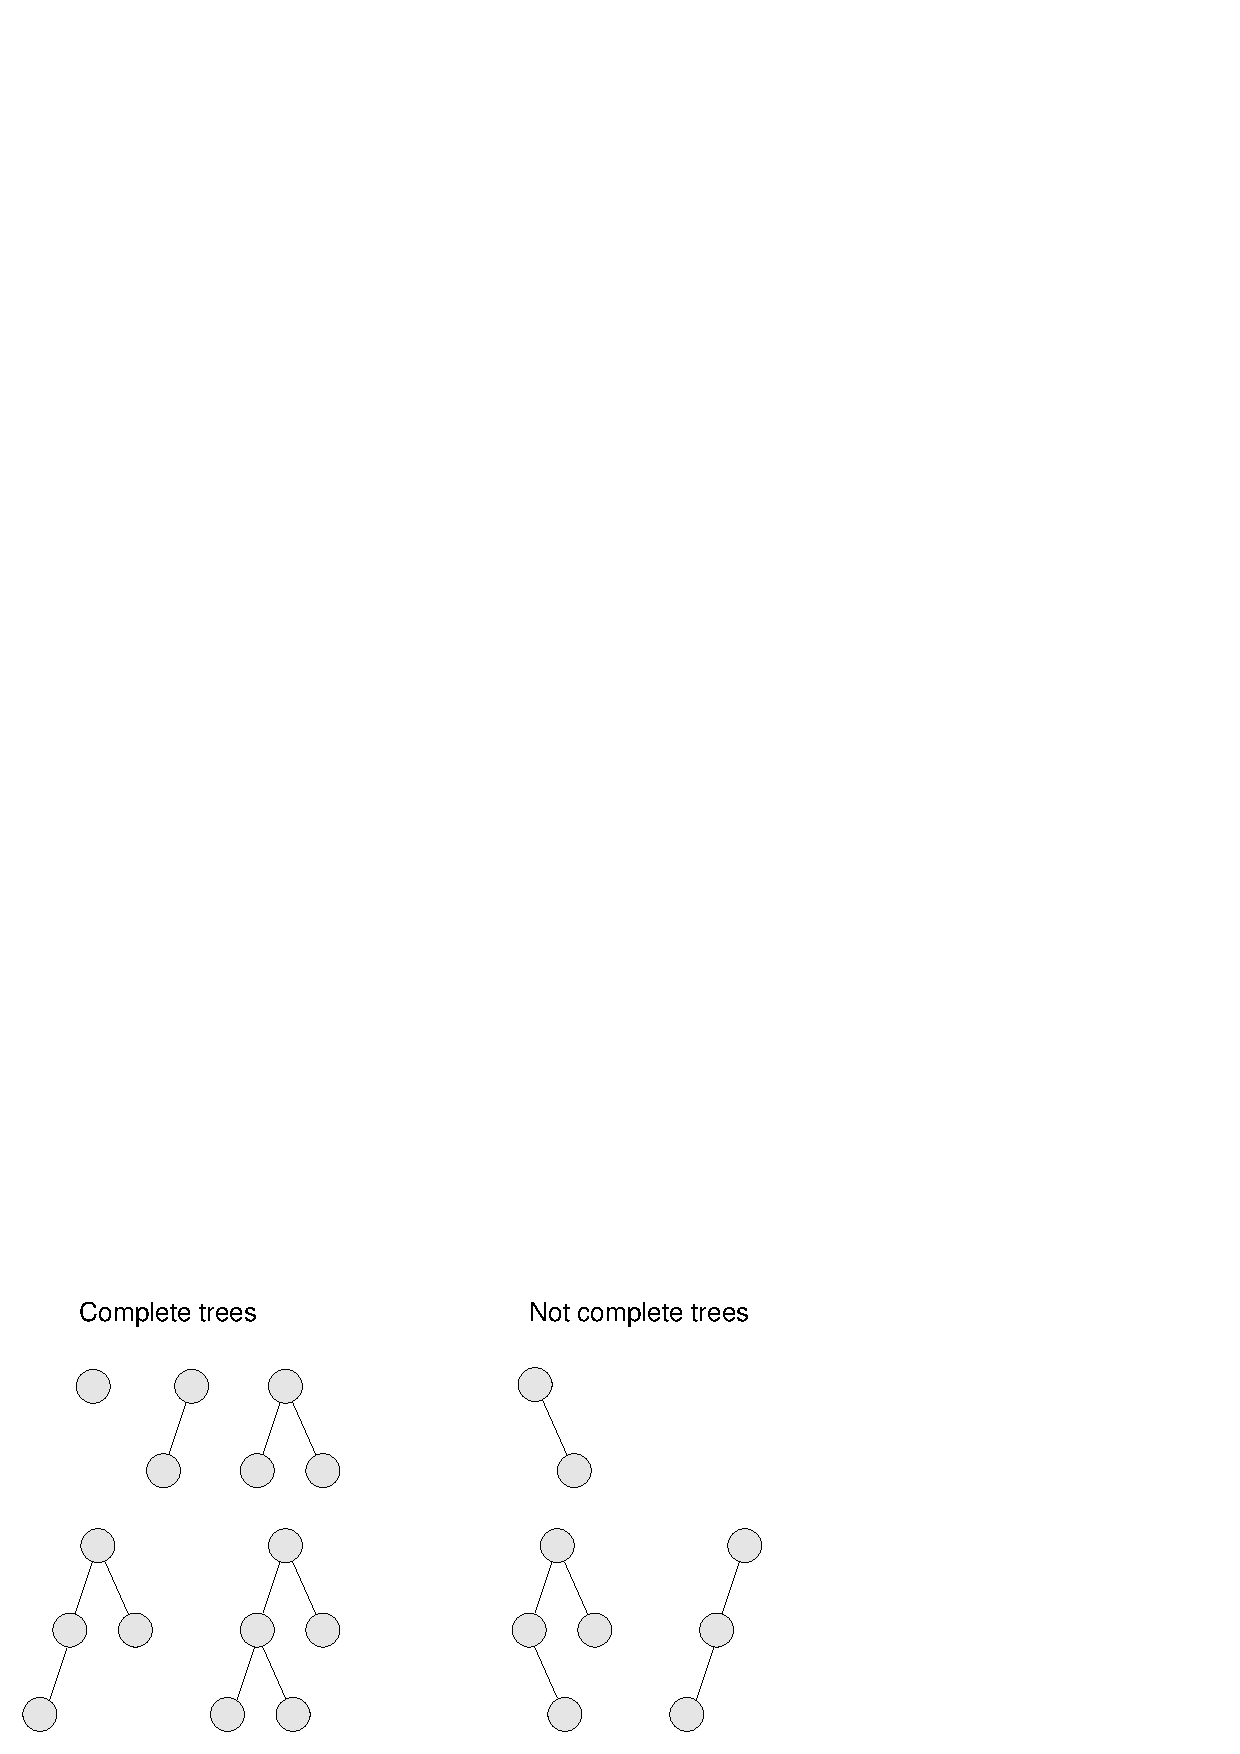
\includegraphics{figs/tree4.pdf}
 
An empty tree is also considered complete.  We can define completeness
more rigorously by comparing the height of the subtrees.  Recall that
the {\bf height} of a tree is the number of levels.

\index{height}

Starting at the root, if the tree is complete, then the
height of the left subtree and the height of the right subtree
should be equal, or the left subtree may be taller by one.
In any other case, the tree cannot be complete.
Furthermore, if the tree is complete, then the height
relationship between the subtrees has to be true for every
node in the tree.

\index{recursive definition}

The {\bf heap property} is similarly recursive.  In order for a
tree to be a heap, the largest value in the tree has to be at
the root, {\em and} the same has to be true for each subtree.
As another exercise, write a method that checks whether a tree
has the heap property.

\begin{exercise}
Write a method that takes a Tree as a parameter and checks
whether it is complete.

HINT: You can use the {\tt height} method from Exercise~\ref{ex.height}.
\end{exercise}

\begin{exercise}
Write a method that takes a Tree as a parameter and checks
whether it has the heap property.
\end{exercise}


\section{Heap {\tt remove}}
\index{reheapify}

It might seem odd that we are going to remove things from the
heap before we add any, but I think removal is easier
to explain.

At first glance, we might think that removing an item from the
heap is a constant time operation, since the item with
the highest priority is always at the root.  The problem is that
once we remove the root node, we are left with something that
is no longer a heap.  Before we can return the result, we have
to restore the heap property.  We call this operation
{\tt reheapify}.

The situation is shown in the following figure:
 
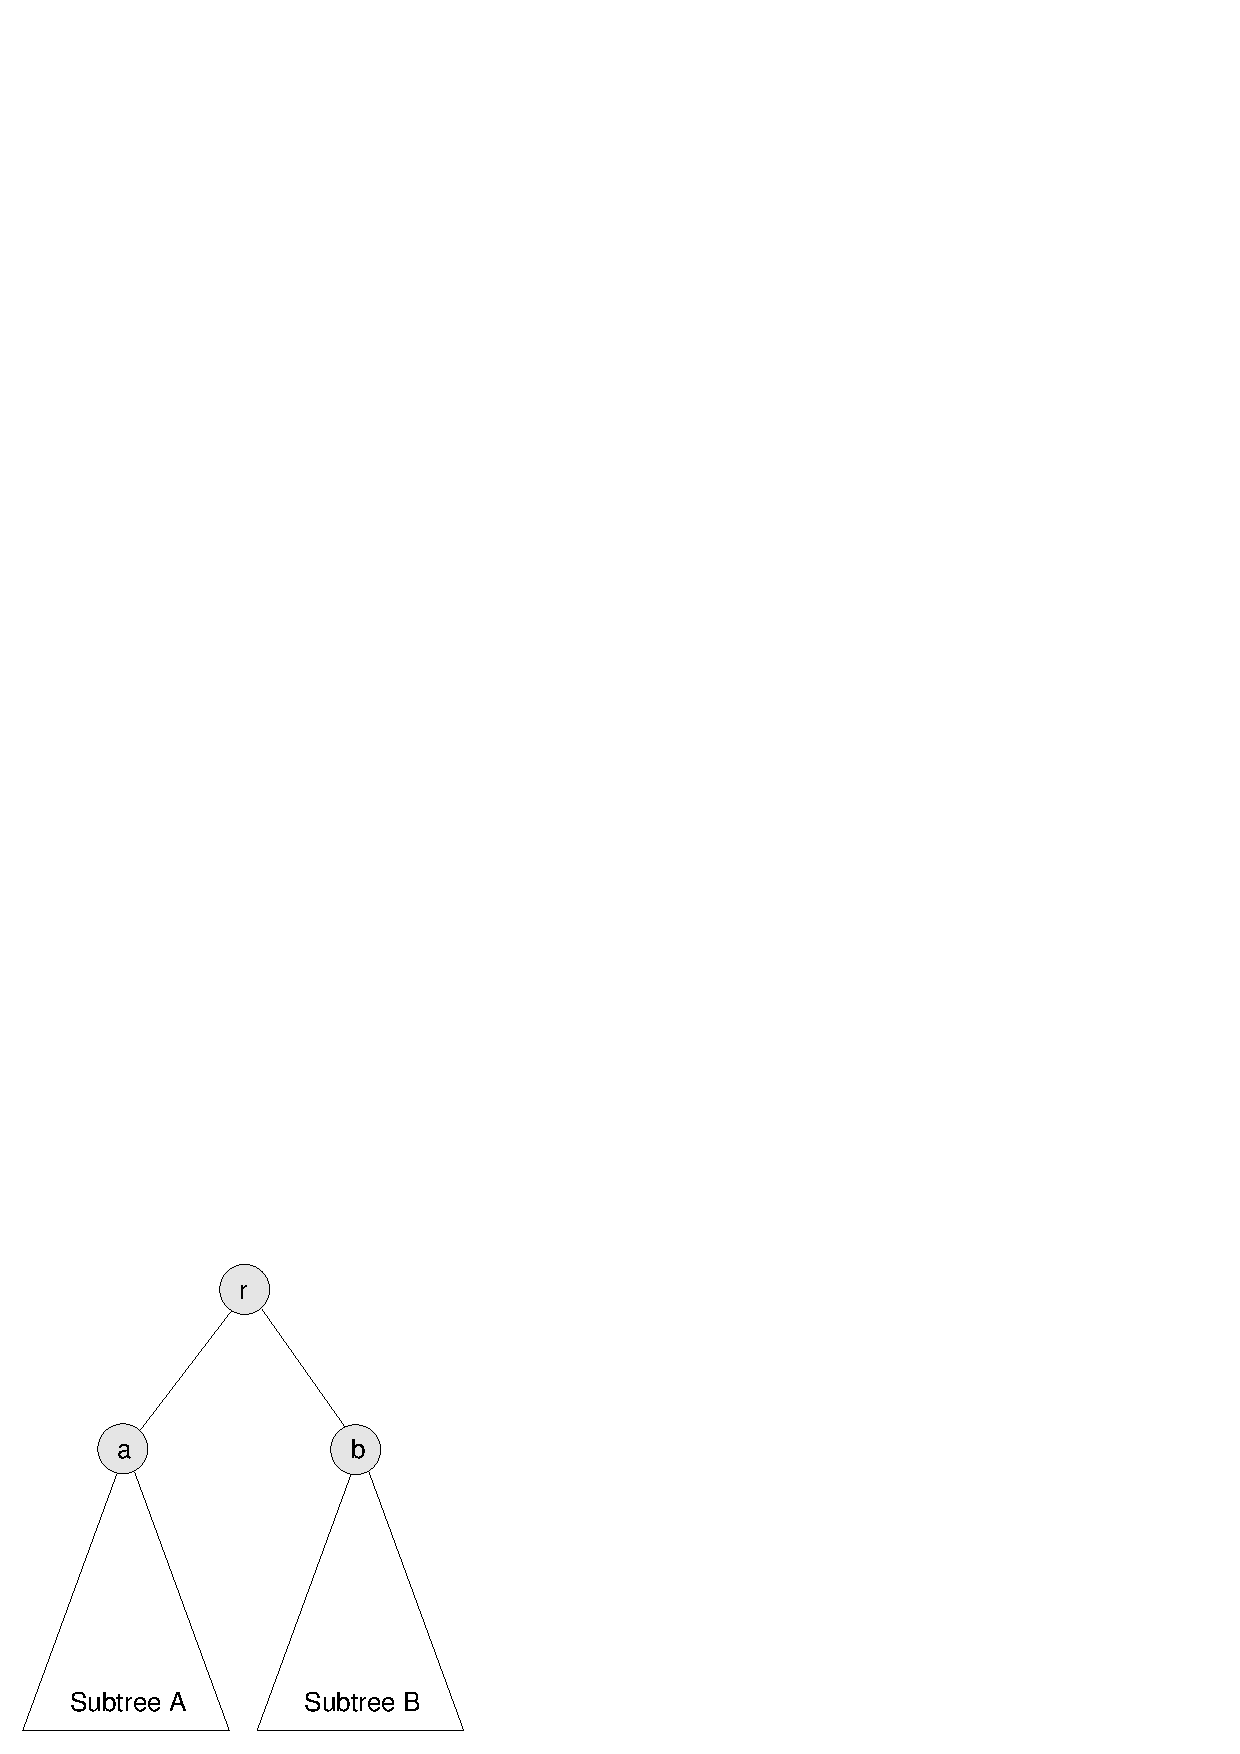
\includegraphics[height=2in]{figs/tree5.pdf}
 
The root node has priority {\tt r} and two subtrees, A and B.
The value at the root of Subtree A is {\tt a} and the value at
the root of Subtree B is {\tt b}.

We assume that before we remove {\tt r} from the tree, the
tree is a heap.  That implies that {\tt r} is the largest value
in the heap and that {\tt a} and {\tt b} are the largest values
in their respective subtrees.

Once we remove {\tt r}, we have to make the resulting tree
a heap again.  In other words we need to make sure it has
the properties of completeness and heapness.

The best way to ensure completeness is to remove the bottom-most,
right-most node, which we'll call {\tt c} and put its value at the
root.  In a general tree implementation, we would have to traverse the
tree to find this node, but in the array implementation, we can find
it in constant time because it is always the last (non-null) element
of the array.

Of course, the chances are that the last value is not the highest,
so putting it at the root breaks the heapness property.  Fortunately
it is easy to restore.  We know that the largest value in the
heap is either {\tt a} or {\tt b}.  Therefore we can select whichever
is larger and swap it with the value at the root.

Arbitrarily, let's say that {\tt b} is larger.  Since we
know it is the highest value left in the heap, we can put it
at the root and put {\tt c} at the top of Subtree B.  Now the
situation looks like this:
 
\includegraphics[height=2in]{figs/tree6.pdf}

Again, {\tt c} is the value we copied from the
last element in the array and {\tt b} is the highest
value left in the heap.  Since we haven't changed Subtree A
at all, we know that it is still a heap.  The only problem is
that we don't know if Subtree B is a heap, since we just stuck
a (probably low) value at its root.

\index{recursion}

Wouldn't it be nice if we had a method that could {\tt reheapify}
Subtree B?  Wait... we do!


\section {Heap {\tt add}}

Adding a new item in a heap is a similar operation, except that
instead of trickling a value down from the top, we trickle it
up from the bottom.

Again, to guarantee completeness, we add the new element at the
bottom-most, rightmost position in the tree, which is the next
available space in the array.

Then to restore the heap property, we compare the new value with
its neighbors.  The situation looks like this:
 
\includegraphics[height=2in]{figs/tree7.pdf}
 
The new value is {\tt c}.  We can restore the heap property
of this subtree by comparing {\tt c} to {\tt a}.  
If {\tt c} is smaller, then the heap property is satisfied.
If {\tt c} is larger, then we swap {\tt c} and {\tt a}.  The
swap satisfies the heap property because we know that {\tt c}
must also be bigger than {\tt b}, because {\tt c > a} and
{\tt a > b}.

Now that the subtree is reheapified, we can work our way up
the tree until we reach the root.


\section {Performance of heaps}
\index{Heap!analysis}
\index{analysis!Heap}

For both add and remove, we perform a constant time operation
to do the actual addion and removal, but then we have to
reheapify the tree.  In one case we start at the root and work
our way down, comparing items and then recursively reheapifying
one of the subtrees.  In the other case we start at a leaf and
work our way up, again comparing elements at each level of
the tree.

As usual, there are several operations we might want to count,
like comparisons and swaps.  Either choice would work; the
real issue is the number of levels of the tree we examine
and how much work we do at each level.  In both cases we
keep examining levels of the tree until we restore the heap
property, which means we might only visit one, or in the worst
case we might
have to visit them all.  Let's consider the worst case.

At each level, we perform only constant time operations
like comparisons and swaps.  So the total amount of work is
proportional to the number of levels in the tree, a.k.a.
the height.

So we might say that these operations are linear with respect to
the height of the tree, but the ``problem size'' we are interested
in is not height, it's the number of items in the heap.

As a function of $n$, the height of the tree is $log_2 n$.
This is not true for all trees, but it is true for complete
trees.  To see why, think of the number of nodes on each level
of the tree.  The first level contains 1, the second contains 2,
the third contains 4, and so on.  The $i$th level contains
$2^i$ nodes, and the total number in all levels up to $i$ is
$2^i - 1$.  In other words, $2^h = n$, which means that
$h = log_2 n$.

\index{logarithmic time}

Thus, both add and remove take {\bf logarithmic} time.
To add and remove $n$ items takes time proportional to
$n \log_2 n$.


\section{Heapsort}
\index{heapsort}
\index{sorting}
\index{analysis!heapsort}

The result of the previous section suggests yet another algorithm
for sorting.  Given $n$ items, we add them into a Heap and
then remove them.  Because of the Heap semantics, they come
out in order.  We have already shown that this algorithm, which
is called {\bf heapsort}, takes time proportional to $n \log_2 n$,
which is better than selection sort and the same as mergesort.

As the value of $n$ gets large, we expect heapsort to be faster
than selection sort, but performance analysis gives us no way
to know whether it will be faster than mergesort.  We would say
that the two algorithms have the same {\bf order of growth} because
their runtimes grow with the same functional form.  Another way to
say the same thing is that they belong to the same {\bf complexity
class}.

\index{big-O notation}
\index{complexity class}
\index{order of growth}
\index{constant time}
\index{linear time}
\index{quadratic time}
\index{logarithmic time}

Complexity classes are sometimes written in ``big-O notation''.
For example, $\mathcal{O} (n^2)$, pronounced ``oh of
en squared'' is the set of all functions that grow no faster
than $n^2$ for large values of $n$.  To say that an algorithm
is $\mathcal{O} (n^2)$ is the same as saying that it
is quadratic.  The other complexity classes we have seen,
in decreasing order of performance, are:

\vspace {0.2in}
\begin{tabular}{ll}
$\mathcal{O} (1)$          &  constant time  \\
$\mathcal{O} (\log n)$     &  logarithmic  \\
$\mathcal{O} (n)$          &  linear  \\
$\mathcal{O} (n \log n)$   &  ``en log en''  \\
$\mathcal{O} (n^2)$        &  quadratic  \\
$\mathcal{O} (2^n)$        &  exponential
\end{tabular}
\vspace {0.2in}

So far none of the algorithms we have looked at are {\bf exponential}.
For large values of $n$, these algorithms quickly become impractical.
Nevertheless, the phrase ``exponential growth'' appears frequently in
even non-technical language.  It is frequently misused so I wanted to
include its technical meaning.

People often use ``exponential'' to describe any curve that is
increasing and accelerating (that is, one that has positive slope and
curvature).  Of course, there are many other curves that fit this
description, including quadratic functions (and higher-order
polynomials) and even functions as undramatic as $n \log n$.  Most
of these curves do not have the (often detrimental) explosive
behavior of exponentials.


\section{Glossary}
\index{selection sort}
\index{mergesort}
\index{heapsort}
\index{complexity class}
\index{order of growth}
\index{overhead}

\begin{description}

\item[selection sort:] The simple sorting algorithm in Section~\ref{sorting}.

\item[mergesort:]  A better sorting algorithm from Section~\ref{mergesort}.

\item[heapsort:]  Yet another sorting algorithm.

\item[complexity class:]  A set of algorithms whose performance
(usually run time) has the same order of growth.

\item[order of growth:]  A set of functions with the same leading-order
term, and therefore the same qualitative behavior for large values
of $n$.

\item[overhead:]  Additional time or resources consumed by a program
performing operations other than the abstract operations considered
in performance analysis.

\end{description}


\section{Exercises}

\begin{exercise}
\begin{enumerate}

\item Draw the Heap represented by the following array.

\includegraphics{figs/heap.pdf}

\item Show what the array would look like after the value
68 is added to the Heap.

\end{enumerate}
\end{exercise}

\begin{exercise}
Assume that there are $n$ elements in a Heap.  To find
the median value of the elements, we could remove $n/2-1$ elements
and then return the value of the $n/2$-eth element.  Then we
would have to put $n/2$ elements back into the Heap.  What would
be the order of growth of this algorithm?
\end{exercise}

\begin{exercise}
How many times will the following loop
execute?  Express your answer as a function of {\tt n}:

\begin{verbatim}
while (n > 1) {
    n = n / 2;
}
\end{verbatim}
\end{exercise}


\begin{exercise}
How many recursive calls will zippo make?  Express
your answer as a function of {\tt x} or {\tt n} or both.

\begin{verbatim}
public static double zippo (double x, int n) {
    if (n == 0) return 1.0;
    return x * zippo (x, n-1);
}
\end{verbatim}
\end{exercise}


\begin{exercise}
Write an implementation of a Heap based on the array implementation
of a tree.  The run time of the {\tt add} and {\tt remove} operations
should be proportional to $\log n$, where $n$ is the number of elements
in the Heap.
\end{exercise}




\chapter{Maps}

\section {Arrays, Vectors and Maps}
\index{array}
\index{Vector}
\index{map}

Arrays are a generally useful data structure, but they suffer
from two important limitations:

\begin{itemize}

\item The size of the array does not depend on the number of
items in it.  If the array is too big, it wastes space.  If
it is too small it might cause an error, or we might have to
write code to resize it.

\item Although the array can contain any type of item, the
indices of the array have to be integers.  We cannot, for
example, use a String to specify an element of an array.

\end{itemize}

In Section~\ref{vector} we saw how the built-in {\tt Vector} class
solves the first problem.  As the client code adds items the Vector
expands automatically.  It is also possible to shrink a Vector so that
the capacity is the same as the current size.

But {\tt Vectors} don't help with the second problem.  The indices are
still integers.  That's where the Map ADT comes in.  A Map is similar
to a Vector; the difference is that it can use any object type as an
index.  These generalized indices are called {\bf keys}.

Just as you use an index to access a value in a Vector, you use a key
to access a value in a Map.  Each key is associated with a value,
which is why Maps are sometimes called {\bf associative arrays}.  The
association of a particular key with a particular value is called an
{\bf entry}.

\index{dictionary}
\index{associative array}
\index{key}
\index{entry}
\index{index}

A common example of a map is a dictionary, which maps
words (the keys) onto their definitions (the
values).  Because of this example Maps are also sometimes called
Dictionaries.  And, just for completeness, Maps are also sometimes
called Tables.


\section {The Map ADT}
\label{map}
\index{Map ADT}
\index{ADT!Map}

Like the other ADTs we have looked at, Maps are defined
by the set of operations they support:

\begin{description}

\item[constructor:] Make a new, empty map. 

\item[{\tt put}:]  Create an entry that associates a value with a key.

\item[{\tt get}:]  For a given key, find the corresponding value.

\item[{\tt containsKey}:]  Return {\tt true} if there
is an entry in the Map with the given Key.

\item[{\tt keySet}]: Returns a Set that contains all the keys
in the Map.

\end{description}


\section {The built-in HashMap}
\index{HashMap}
\index{class!HashMap}

Java provides an implementation of the Map ADT called
{\tt java.util.HashMap}.
Later in the chapter we'll see why it is called {\tt HashMap}.

To demonstrate the use of a HashMap we'll write
a short program that traverses a String and counts the number
of times each word appears.

We'll create a new class called {\tt WordCount} that will
build the Map and then print its contents.  Each
{\tt WordCount} object contains a {\tt HashMap} as an
instance variable:

\begin{verbatim}
public class WordCount {
    HashMap map;

    public WordCount () {
        map = new HashMap ();
    }
}
\end{verbatim}
%
The only public methods for {\tt WordCount} are {\tt processLine},
which takes a String and adds its words to the Map, and {\tt print},
which prints the results at the end.

{\tt processLine} breaks the String into words using a 
{\tt StringTokenizer} and passes each word to {\tt processWord}.

\begin{verbatim}
    public void processLine (String s) {
        StringTokenizer st = new StringTokenizer (s, " ,.");
        while (st.hasMoreTokens()) {
            String word = st.nextToken();
            processWord (word.toLowerCase ());
        }
    }
\end{verbatim}
%
The interesting work is in {\tt processWord}.

\begin{verbatim}
    public void processWord (String word) {
        if (map.containsKey (word)) {
            Integer i = (Integer) map.get (word);
            Integer j = new Integer (i.intValue() + 1);
            map.put (word, j);
        } else {
            map.put (word, new Integer (1));
        }
    }
\end{verbatim}
%
If the word is already in the map, we {\tt get} its counter,
increment it, and {\tt put} the new value.  Otherwise, we just
{\tt put} a new entry in the map with the counter set to {\tt 1}.


\index{The keySet}
\index{{\tt keySet}}
\index{traverse}

To print the entries in the map, we need to be able to traverse the
keys in the map.  Fortunately, {\tt HashMap}
provides a method, {\tt keySet}, that returns a {\tt Set}
object, and {\tt Set} provides a method {\tt iterator} that returns
(you guessed it) an Iterator.

Here's how to use {\tt keySet} to print the contents of the {\tt
HashMap}:

\begin{verbatim}
public void print () {
    Set set = map.keySet();
    Iterator it = set.iterator();
    while (it.hasNext ()) {
        String key = (String) it.next ();
        Integer value = (Integer) map.get (key);
        System.out.println ("{ " + key + ", " + value + " }"); 
    }
}    
\end{verbatim}
%
Each of the elements of the Iterator is an Object,
but since we know they are keys, we typecast them to be Strings.
When we get the values from the Map, they are also Objects,
but we know they are counters, so we typecast them to be Integers.

Finally, to count the words in a string:

\begin{verbatim}
        WordCount wc = new WordCount ();
        wc.processLine ("you spin me right round baby " +
                        "right round like a record baby " +
                        "right round round round");
        wc.print ();
\end{verbatim}
%
The output is

\begin{verbatim}
{ you, 1 }
{ round, 5 }
{ right, 3 }
{ me, 1 }
{ like, 1 }
{ baby, 2 }
{ spin, 1 }
{ record, 1 }
{ a, 1 }
\end{verbatim}
%
The elements of the Iterator are not in any particular order.
The only guarantee is that all the keys in the map will appear.


\section {A Vector implementation}
\index{implementation!Map}
\index{map!vector implementation}
\index{Entry}

An easy way to implement the Map ADT is to use a {\tt Vector}
of entries, where each Entry is an object that contains a key
and a value.
A class definition for {\tt Entry} might look like
this:

\begin{verbatim}
class Entry {
    Object key, value;

    public Entry (Object key, Object value) {
        this.key = key;
        this.value = value;
    }

    public String toString () {
        return "{ " + key + ", " + value + " }";
    }
}
\end{verbatim}
%
Then the implementation of Map looks like this:

\begin{verbatim}
public class MyMap {
    Vector entries;

    public Map () {
        entries = new Vector ();
    }
}
\end{verbatim}

To put a new entry in the map, we just {\tt add} a new
{\tt Entry} to the {\tt Vector}:

\begin{verbatim}
    public void put (Object key, Object value) {
        entries.add (new Entry (key, value));
    }
\end{verbatim}

Then to look up a key in the Map we have to traverse the
Vector and find an Entry with a matching
key:

\begin{verbatim}
    public Object get (Object key) {
        Iterator it = entries.iterator ();
        while (it.hasNext ()) {
            Entry entry = (Entry) it.next ();
            if (key.equals (entry.key)) {
                return entry.value;
            }
        }
        return null;
    }
\end{verbatim}
%
The idiom to traverse a {\tt Vector} is the one we saw in
Section~\ref{iterator}.  When we compare keys, we use deep
equality (the {\tt equals} method) rather than shallow
equality (the {\tt ==} operator).  This allows the key class
to specify the definition of equality.  In the example, the
keys are Strings, so {\tt get} will use the {\tt equals}
method in the {\tt String} class.

\index{traverse} 
\index{deep equality}
\index{quality!deep}
\index{shallow equality}
\index{quality!shallow}

For most of the built-in classes, the {\tt equals} method
implements deep equality.  For some classes, though, it is
not easy to define what that means.  For example, see the
documentation of {\tt equals} for {\tt Doubles}.

\index{equals}
\index{equality}

Because {\tt equals} is an object method, this implementation
of {\tt get} does not work if a key is {\tt null}.  In order to
handle {\tt null} keys, we would have to add a special case to
{\tt get} or write a class method that compares keys and handles
{\tt null} parameters safely.  But we will skip this detail.

Now that we have {\tt get}, we can write a version of {\tt put} that
is more complete.  If there is already an entry in the map with the
given key, {\tt put} is supposed to update it (give it a new value),
and return the old value (or {\tt null} if there was none).  Here is
an implementation that provides this feature:

\begin{verbatim}
    public Object put (Object key, Object value) {
        Object result = get (key);
        if (result == null) {
            Entry entry = new Entry (key, value);
            entries.add (entry);
        } else {
            update (key, value);
        }
        return result;
    }

    private void update (Object key, Object value) {
        Iterator it = entries.iterator ();
        while (it.hasNext ()) {
            Entry entry = (Entry) it.next ();
            if (key.equals (entry.key)) {
                entry.value = value;
                break;
            }
        }
    }
\end{verbatim}

The {\tt update} method is not part of the Map ADT, so
it is declared {\tt private}.  It traverses the vector until
it finds the right {\tt Entry} and then it updates
the {\tt value} field.  Notice that we don't modify
the {\tt Vector} itself, just one of the objects it contains.

The only methods we haven't implemented are {\tt containsKey} and {\tt
keySet}.  The {\tt containsKey} method is almost identical to {\tt get}
except that it returns {\tt true} or {\tt false} instead of an object
reference or {\tt null}.

\begin{exercise}
Implement {\tt keySet} by building and returning a {\tt TreeSet}
object.  Use your implementation of {\tt TreeSet} from
Exercise~\ref{ex.treeset} or the built-in implementation {\tt
java.util.TreeSet}.
\end{exercise}


\section{The {\tt List} metaclass}
\index{metaclass!List} \index{List metaclass}

The {\tt java.util} package defines a metaclass called
{\tt List} that specifies the set of operations a class has to
implement in order to be considered (very abstractly) a list.
This does not mean, of course, that every class that implements
{\tt List} has to be a linked list.

Not surprisingly, the built-in {\tt LinkedList} class is a member of
the {\tt List} metaclass.  Surprisingly, so is {\tt Vector}.

The methods in the {\tt List} definition include {\tt add}, {\tt get}
and {\tt iterator}.  In fact, all the methods from the {\tt Vector}
class that we used to implement {\tt Map} are defined in the {\tt
List} metaclass.  That means that instead of a {\tt Vector}, we could
have used any {\tt List} class.  In our implementation of {\tt Map} we
can replace {\tt Vector} with {\tt LinkedList}, and the program still
works!

This kind of type generality can be useful for tuning
the performance of a program.  You can write the program in
terms of a metaclass like {\tt List} and then test the
program with several different implementations to see which
yields the best performance.


\section{HashMap implementation}
\index{implementation!Map}
\index{implementation!HashMap}
\index{HashMap!implementation}
\index{map!HashMap implementation}

The reason that the built-in implementation of the Map ADT
is called {\tt HashMap} is that it uses a particularly efficient
implementation of a Map called a hash table.

In order to understand the hash table implementation, and why it is
considered efficient, we'll start by analyzing the performance of the
{\tt List} implementation.

Looking at the implementation of {\tt put}, we see that there are
two cases.  If the key is not already in the map, then we
only have to create a new entry and {\tt add} it to
the {\tt List}.  Both of these are constant-time operations.

In the other case, we have to traverse the {\tt List} to find
the existing entry.  That's a linear time operation.
For the same reason, {\tt get} and {\tt containsKey} are also
linear.

Although linear operations are often good enough, we can do
better.  It turns out that there is a way to implement the
Map ADT so that both {\tt put} and {\tt get} are constant time
operations!

The key is to realize that traversing a list takes time
proportional to the length of the list.  If we can put an upper
bound on the length of the list, then we can put an upper
bound on the traverse time, and anything with a fixed upper
bound is considered constant time.

\index{analysis!hash table}

But how can we limit the length of the lists without limiting
the number of items in the map?  By increasing the number
of lists.  Instead of one long list, we'll keep many short
lists.

As long as we know which list to search, we can put a bound
on the amount of searching.


\section{Hash Functions}
\index{hash function}
\index{mapping}

And that's where hash functions come in.  We need some way to look at
a key and know, without searching, which list it will be in.  We'll
assume that the lists are in an array (or {\tt Vector}) so we can
refer to them by index.

The solution is to come up with some mapping---almost any
mapping---between the key values and the indices of the lists.
For every possible key there has to be a single index, but
there might be many keys that map to the same index.

For example, imagine an array of 8 Lists and a map made
up of keys that are {\tt Integers} and values that are
{\tt Strings}.  It might be tempting to use the
{\tt intValue} of the {\tt Integers} as indices, since they
are the right type, but there are a whole lot of integers
that do not fall between 0 and 7, which are the only legal
indices.

\index{modulus}
\index{operator!modulus}

The modulus operator provides a simple
(in terms of code) and efficient (in terms of run time) way
to map {\em all} the integers into the range $(0, 7)$.
The expression

\begin{verbatim}
    key.intValue() % 8
\end{verbatim}
%
is guaranteed to produce a value in the range from -7 to 7 (including
both).  If you take its absolute value (using {\tt Math.abs}) you
will get a legal index.

For other types, we can play similar games.  For example,
to convert a {\tt Character} to an integer, we can use
the built-in method {\tt Character.getNumericValue} and
for {\tt Doubles} there is {\tt intValue}.

\index{shifted sum}

For {\tt Strings} we could get the numeric value of each character and
add them up, or instead we might use a {\bf shifted sum}.  To
calculate a shifted sum, you alternate between adding new values to
the accumulator and shifting the accumulator to the left.  By ``shift
to the left'' I mean ``multiply by a constant.''

To see how this works, take the list of numbers
${ 1, 2, 3, 4, 5, 6 }$ and compute their shifted sum as
follows.  First, initialize the accumulator to 0.  Then,

\begin{enumerate}

\item Multiply the accumulator by 10.

\item Add the next element of the list to the accumulator.

\item Repeat until the list is finished.

\end{enumerate}

As an exercise, write a method that calculates the shifted sum
of the numeric values of the characters in a {\tt String} using
a multiplier of 16.

For each type, we can come up with a function that takes values of that
type and generates a corresponding integer value.  These
functions are called {\bf hash functions}, because they often
involve making a hash of the components of the object.  The
integer value for each object is called its {\bf hash code}.

There is one other way we might generate a hash code for Java objects.
Every Java object provides a method called {\tt hashCode} that returns
an integer that corresponds to that object.  For the built-in types,
the {\tt hashCode} method is implemented so that if two objects
contain the same data (deep equality), they will have the same hash
code.  The documentation of these methods explains what the hash
function is.  You should check them out.

\index{deep equality}
\index{hash function}
\index{hash code}

For user-defined types, it is up to the implementor to provide
an appropriate hash function.  The default hash function, provided
in the {\tt Object} class, often uses the location of the
object to generate a hash code, so its notion of ``sameness''
is shallow equality.  Most often when we are searching a
Map for a key, shallow equality is not what we want.

Regardless of how the hash code is generated, the last step
is to use modulus and absolute value functions to map the hash code
into the range of legal indices.


\section{Resizing a hash map}
\index{resizing}
\index{hash map!resizing}

Let's review.  A hash table consists of an array (or Vector)
of {\tt Lists}, where each {\tt List} contains a small number
of entries.  To add a new entry to a map, we calculate
the hash code of the new key and add the entry to the
corresponding {\tt List}.

To look up a key, we hash it again and search the corresponding list.
If the lengths of the lists are bounded then the search time is
bounded.

So how do we keep the lists short?  Well, one goal is to keep
them as balanced as possible, so that there are no very long
lists at the same time that others are empty.
This is not easy to do perfectly---it depends on how well we
chose the hash function---but we can usually do a pretty good
job.

Even with perfect balance, the average list length
grows linearly with the number of entries, and we have to put
a stop to that.

The solution is to keep track of the average number of entries
per list, which is called the {\bf load factor};
if the load factor gets too high, we have to resize the hash table.

\index{load factor}
\index{rehashing}

To resize, we create a new hash table, usually twice as big as the
original, take all the entries out of the old one, hash them again,
and put them in the new hash table.  Usually we can get away with
using the same hash function; we just use a different value for the
modulus operator.


\section{Performance of resizing}
\index{analysis!HashMap}

How long does it take to resize the hash table?  Clearly it is linear
with the number of entries.  That means that {\em most} of the
time {\tt put} takes constant time, but every once in a while
---when we resize---it takes linear time.

At first that sounds bad.  Doesn't that undermine my
claim that we can perform {\tt put} in constant time?  Well,
frankly, yes.  But with a little wheedling, we can fix it.

Since some {\tt put} operations take longer than others, let's
figure out the {\em average} time for a put operation.  The
average is going to be $c$, the constant time for a simple
{\tt put}, plus an additional term of $p$, the percentage of
the time I have to resize, times $kn$, the cost
of resizing.
%
\begin{equation}
t(n) = c + p \cdot kn
\end{equation}
%
We don't know what $c$ and $k$ are, but we can figure out what
$p$ is.  Imagine that we have just resized the hash map by
doubling its size.  If there are $n$ entries, then we can add an
addition $n$ entries before we have to resize again.  So the
percentage of the time we have to resize is $1/n$.

Plugging into the equation, we get
%
\begin{equation}
t(n) = c + 1/n \cdot kn = c + k
\end{equation}
%
In other words, $t(n)$ is constant time!


\section{Glossary}
\index{map}
\index{entry}
\index{key}
\index{value}
\index{dictionary}
\index{associative array}
\index{hash map}
\index{hash function}
\index{hash code}
\index{shifted sum}
\index{load factor}

\begin{description}

\item[map:] An ADT that defines operations on a collection of
entries.

\item[entry:] An element in a map that contains a key and a value.

\item[key:] An index, of any type, used to look up values in a map.

\item[value:] An element, of any type, stored in a map.

\item[dictionary:] Another name for a map.

\item[associative array:] Another name for a dictionary.

\item[hash map:] A particularly efficient implementation of a map.

\item[hash function:] A function that maps values of a certain type
onto integers.

\item[hash code:] The integer value that corresponds to a given value.

\item[shifted sum:] A simple hash function often used for compounds
objects like {\tt Strings}.

\item[load factor:] The number of entries in a hashmap divided
by the number of lists in the hashmap; i.e. the average number
of entries per list.


\end{description}

\section{Exercises}

\begin{exercise}
\begin{enumerate}
\item Compute the shifted sum of the numbers 1, 2, 3, 4, 5, 6 using
a multiplier of 10.

\item Compute the shifted sum of the numbers 11, 12, 13, 14, 15, 16 using
a multiplier of 100.

\item Compute the shifted sum of the numbers 11, 12, 13, 14, 15, 16 using
a multiplier of 10.
\end{enumerate}
\end{exercise}


\begin{exercise}
Imagine you have a hash table that
contains 100 lists.  If you are asked to {\tt get} the value associated
with a certain key, and the hash code for that key is 654321, what is
the index of the list where the key will be (if it is in the map)?
\end{exercise}


\begin{exercise}
If there are 100 lists and there are 89 entries in the
map and the longest list contains 3 entries, and the median
list length is 1 and 19\% of the lists are empty, what is the load
factor?
\end{exercise}


\begin{exercise}
Imagine that there are a large number of people at a party.
You would like to know whether any two of them have the same
birthday.  First, you design a new kind of Java object that
represents birthdays with two instance variables:
{\tt month}, which is an integer between 1 and 12, and
{\tt day}, which is an integer between 1 and 31.

Next, you create an array of {\tt Birthday} objects that
contains one object for each person at the party, and you
get someone to help type in all the birthdays.

\begin{enumerate}

\item Write an {\tt equals} method for {\tt Birthday} so that
Birthdays with the same month and day are equal.

\item Write a method called {\tt hasDuplicate} that takes
an array of {\tt Birthdays} and returns {\tt true} if there
are two or more people with the same birthday.
Your algorithm should only traverse the array of
{\tt Birthdays} once.

\item Write a method called {\tt randomBirthdays} that takes
an integer {\tt n} and returns an array with {\tt n} random
{\tt Birthday} objects.  To keep things simple, you can pretend
that all months have 30 days.

\item Generate 100 random arrays of 10 {\tt Birthdays} each, and
see how many of them contain duplicates.

\item If there are 20 people at a party, what is the probability
that two or more of them have the same birthday?

\end{enumerate}
\end{exercise}


\begin{exercise}
A Map is said to be {\bf invertible} if each key and each value
appears only once.  In a HashMap, it is always true that each
key appears only once, but it is possible for the same value to
appear many times.  Therefore, some HashMaps are invertible
and some are not.

Write a method called {\tt isInvertible} that takes a {\tt HashMap}
and returns true if the map is invertible and false otherwise.
\end{exercise}


\begin{exercise}

The goal of this exercise is to find the 20 most common words in this
book.  Type in the code from the book that uses the built-in {\tt
HashMap} to count word frequencies.  Download the text of the book
from \url{http://thinkapjava.com/thinkapjava.txt}.

The plain text version of the book is generated automatically by a
program called {\tt detex} that tries to strip out all the typesetting
commands, but it leaves behind assorted junk.  Think about how your
program should handle punctuation and any other wierdness that appears
in the file.

Write programs to answer the following questions:

\begin{enumerate}

\item How many words are there in the book?

\item How many {\em different} words are there in the book?  For
purposes of comparison, there are (very roughly) 500,000 words in
English, of which (very roughly) 50,000 are in current use.  What
percentage of this vast lexicon did I find fit to use?

\item How many times does the word ``encapsulation'' appear?

\item What are the 20 most common words in the book?  HINT: there is
another data structure that might help with this part of the exercise.

\end{enumerate}
\end{exercise}


\begin{exercise}
Write a method for the {\tt LinkedList} class that checks whether
the list contains a loop.  You should not assume that the length
field is correct.
Your method should be linear in the
number of nodes.
\end{exercise}


\begin{exercise}
Write a hash table implementation of the Map ADT (as defined in
Section~\ref{map}).  Test it by using it with any of the programs
you have written so far.  Hints:

\begin{enumerate}

\item Start with the {\tt Vector} implementation in the book
and make sure it works with existing programs.

\item Modify the implementation to use either an array of
LinkedLists or a Vector of LinkedLists, whichever you prefer.

\end{enumerate}
\end{exercise}


\begin{exercise}
Write an implementation of the {\tt Set} interface using a
{\tt HashMap}.
\end {exercise}


\begin{exercise}
\index{tree!search}
\index{search tree}
\index{binary search tree}

The {\tt java.util} package provides two implementations of the
{\tt Map} interface, called {\tt HashMap} and {\tt TreeMap}.
{\tt HashMap} is based on a hash table like the one described
in this chapter.  {\tt TreeMap} is based on a red-black tree, which
is similar to the search tree in Exercise~\ref{ex.searchtree}.

Although these implementations provide the same interface, we
expect them to achieve different performance.  As the number of
entries, $n$, increases, we expect {\tt add} and {\tt contains}
to take constant time for the hash table implementation, and
logarithmic time for the tree implementation.

Perform an experiment to confirm (or refute!) these performance
predictions.  Write a program that adds $n$ entries to a 
{\tt HashMap} or {\tt TreeMap}, then invokes {\tt contains} on
each of the keys.  Record the runtime of the program for a range
of values of $n$ and make a plot of runtime versus $n$.  Is
the performance behavior in line with our expectations.
\end {exercise}


\chapter{Markov analysis}
\label{markov}

Translate the random text example from Think Python into Java.


\chapter{Huffman code}
\label{huffman}

\section{Variable-length codes}

If you are familiar with Morse code, you know that it is a system
for encoding the letters of the alphabet as a series of dots and
dashes.  For example, the famous signal {\tt ...---...} represents
the letters SOS, which comprise an internationally-recognized call
for help.  This table shows the rest of the codes:

\begin{verbatim}
     A  .-          N  -.          1  .----       .  .-.-.-
     B  -...        O  ---         2  ..---       ,  --..--
     C  -.-.        P  .--.        3  ...--       ?  ..--..
     D  -..         Q  --.-        4  ....-       (  -.--.
     E  .           R  .-.         5  .....       )  -.--.-
     F  ..-.        S  ...         6  -....       -  -....-
     G  --.         T  -           7  --...       "  .-..-.
     H  ....        U  ..-         8  ---..       _  ..--.-
     I  ..          V  ...-        9  ----.       '  .----.
     J  .---        W  .--         0  -----       :  ---...
     K  -.-         X  -..-        /  -..-.       ;  -.-.-.
     L  .-..        Y  -.--        +  .-.-.       $  ...-..-
     M  --          Z  --..        =  -...-
\end{verbatim}

\index{Morse code}
\index{code!Morse}

Notice that some codes are longer than others.  By design, the
most common letters have the shortest codes.  Since there are a
limited number of short codes, that means that less common
letters and symbols have longer codes.  A typical message will
have more short codes than long ones, which minimizes the average
transmission time per letter.

\index{Huffman code}
\index{code!Huffman}
\index{variable-length code}
\index{code!variable-length}

Codes like this are called variable-length codes.  In this chapter,
we will look at an algorithm for generating a variable-length code
called a {\bf Huffman code}.  It is an interesting algorithm in
its own right, but it also makes a useful exercise because its
implementation uses many of the data structures we have been studying.

Here is an outline of the next few sections:

\begin{itemize}

\item First, we will use a sample of English text to generate
a frequency table.  A frequency table is like a histogram; it counts
the number of times each letter appears in the sample text.

\item The heart of a Huffman code is the Huffman tree.  We will
use the frequency table to build the Huffman tree, and then use
the tree to encode and decode sequences.

\item Finally, we will traverse the Huffman tree and built a code
table, which contains the sequence of dots and dashes for each letter.

\end{itemize}


\section {The frequency table}
\label{freqtab}

\index{Poe, Edgar Allen}
\index{Gold Bug, The}
\index{frequency}

Since the goal is to give short codes to common letters, we have to
know how often each letter occurs.  In Edgar Allen Poe's short story
``The Gold Bug,'' one of the characters uses letter frequencies to
crack a cypher.  He explains,

\begin{quote}
``Now, in English, the letter which most frequently occurs is
e. Afterwards, the succession runs thus: a o i d h n
r s t u y c f g l m w b k p q x z.  E however
predominates so remarkably that an individual
sentence of any length is rarely seen, in which it is
not the prevailing character.''
\end{quote}

So our first mission is to see whether Poe got it right.  To check,
I chose as my sample the text of ``The Gold Bug'' itself, which
I downloaded from one of the Web sites that take advantage
of its entry into the public domain.

\begin{exercise}
Write a class called {\tt FreqTab} that counts the number of
times each letter appears in a sample text.  Download the text
of your favorite public-domain short story, and analyse the frequency
of the letters.

\index{HashMap}
\index{class!HashMap}

I found it most convenient to make {\tt FreqTab} extend
{\tt HashMap}.  Then I wrote a method called {\tt increment}
that takes a letter as a parameter and either adds or updates
an entry in the HashMap for each letter.

You can use {\tt keySet} to get the entries from the HashMap,
and print a list of letters with their frequencies.  Unfortunately,
they will not appear in any particular order.  The next exercise
solves that problem.
\end{exercise}


\begin{exercise}
\label{ex.pair}
Write a class called {\tt Pair} that represents a letter-frequency
pair.  Pair objects should contain a letter and a frequency as
instance variables.  {\tt Pair} should implement {\tt Comparable},
where the Pair with the higher frequency wins.

\index{Pair}
\index{class!Pair}

Now sort the letter-frequency pairs from the HashMap by traversing the
set of keys, building {\tt Pair} objects, adding the Pairs to a
PriorityQueue, removing the Pairs from the PriorityQueue, and printing
them in descending order by frequency.

How good was Poe's guess about the most frequent letters?
\end{exercise}


\section{The Huffman Tree}
\label{hufftree}

The next step is to assemble the Huffman tree.  Each node
of the tree contains a letter and its frequency, and pointers to
the left and right nodes.

To assemble the Huffman tree, we start by creating a set of
singleton trees, one for each entry in the frequency table.
Then we build the tree from the bottom up, starting with the
least-frequent letters and iteratively joining subtrees until
we have a single tree that contains all the letters.

Here is the algorithm in more detail.

\begin{enumerate}

\item For each entry in the frequency table, create a singleton
Huffman tree and add it to a PriorityQueue.  When we remove a tree from
the PriorityQueue, we get the one with the lowest frequency.

\item Remove two trees from the PriorityQueue and join them by creating
a new parent node that refers to the removed nodes.  The frequency
of the parent node is the sum of the frequencies of the children.

\item If the PriorityQueue is empty, we are done.  Otherwise, put the
new tree into the PriorityQueue and go to Step 2.

\end{enumerate}

An example will make this clearer.  To keep things managable,
we will use a sample text that only contains the letters
{\tt adenrst}:

\begin{quote}
Eastern Tennessee anteaters ensnare and eat red ants, detest ant
antennae (a tart taste) and dread Antarean anteater-eaters.
Rare Andean deer eat tender sea reeds, aster seeds and rats'
ears.  Dessert?  Rats' asses.
\end{quote}

This eloquent treatise on the eating habits of various fauna
yields the following frequency table:

\begin{verbatim}
e       40
a       32
t       24
s       22
n       20
r       19
d       13
\end{verbatim}

So after Step 1, the PriorityQueue looks like this:

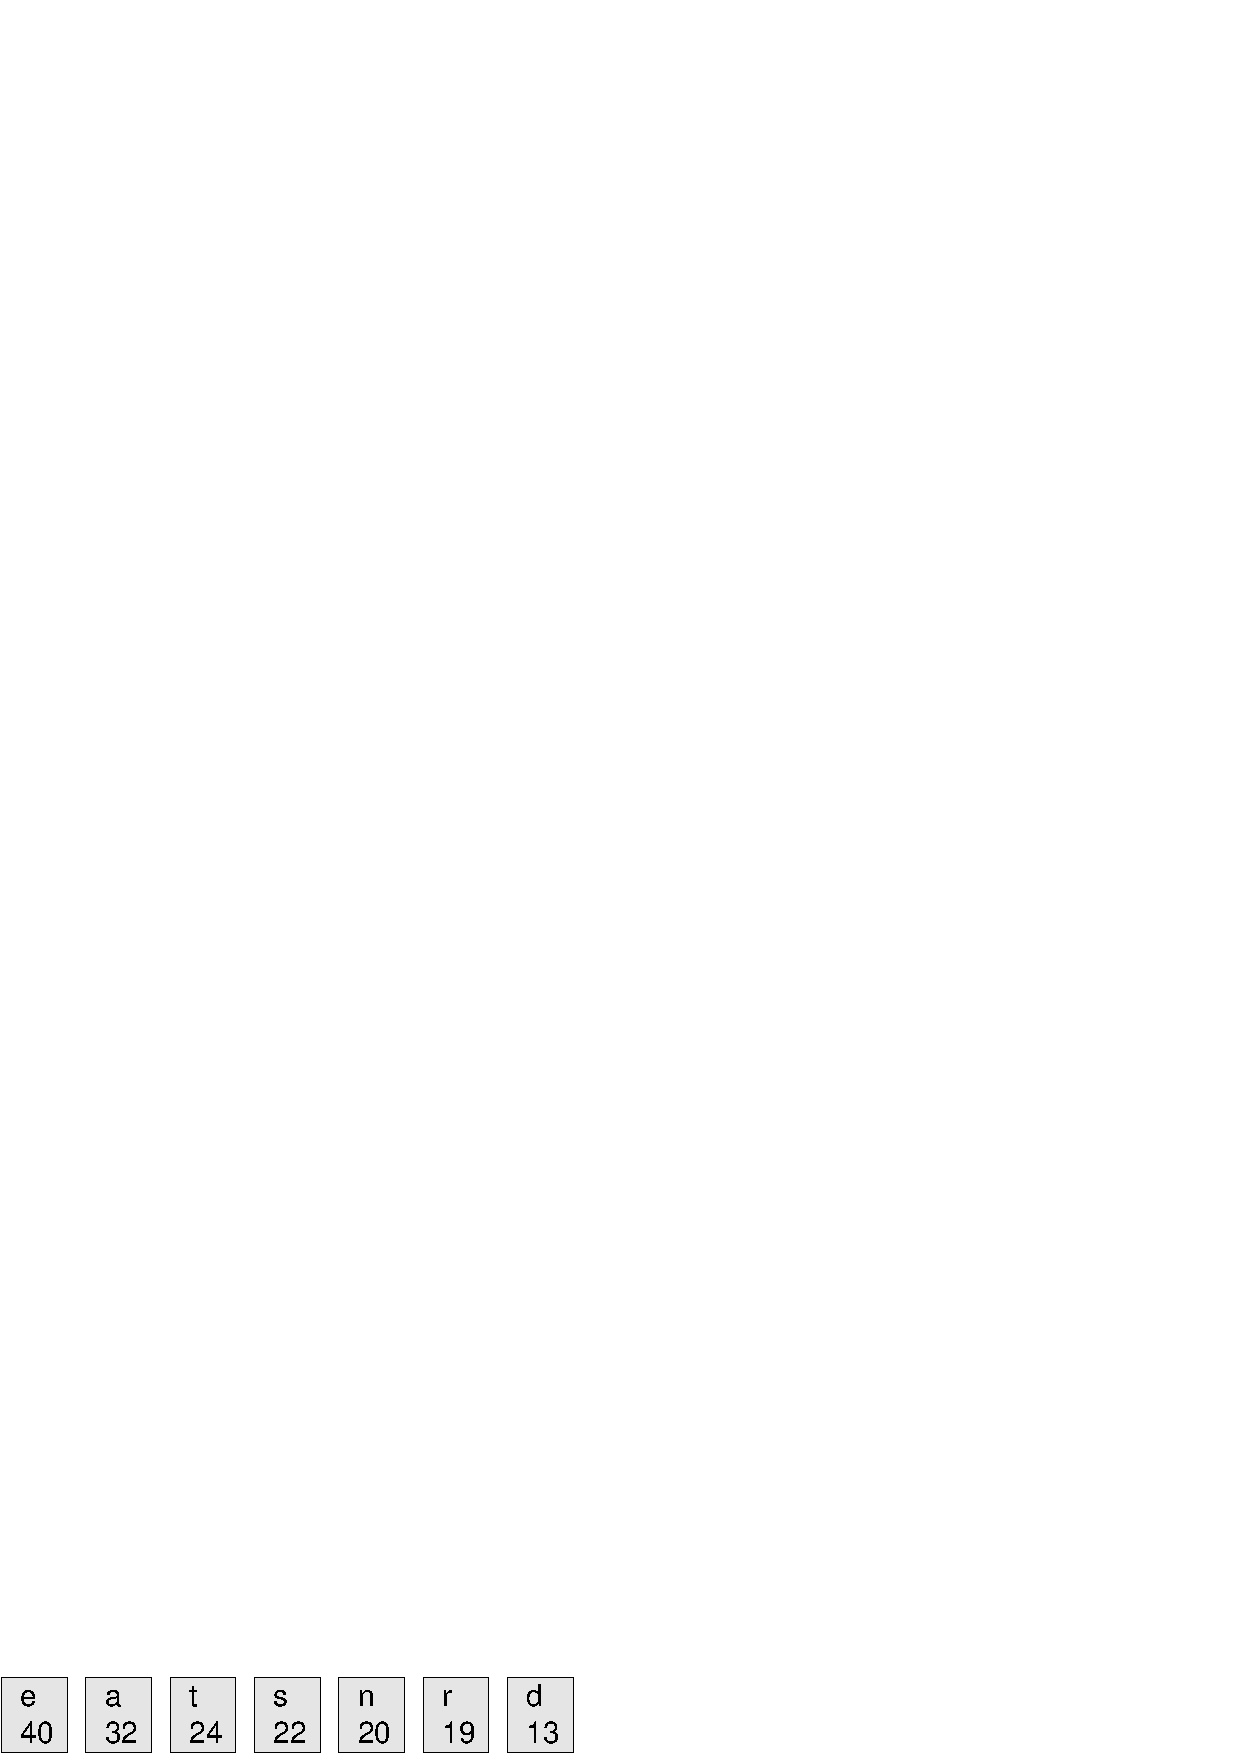
\includegraphics[width=2.0in]{figs/huff0.pdf}

In Step 2, we remove the two trees with the lowest frequency
({\tt r} and {\tt d}) and join them by creating a parent node
with frequency 32.  The letter value for the internal nodes is
irrelevant, so it is omitted from the figures.  When we put the
new tree back in the PriorityQueue, the result looks like this:

\includegraphics[width=2.0in]{figs/huff1.pdf}

Now we repeat the process, combining {\tt s} and {\tt n}:

\includegraphics[width=2.0in]{figs/huff2.pdf}

After the next interation, we have the following collection of
trees.  By the way, a collection of trees is called a {\bf forest}.

\index{forest}

\includegraphics[width=2.0in]{figs/huff3.pdf}

%\includegraphics{figs/huff4.pdf,width=2.0in}
%\includegraphics{figs/huff5.pdf,width=2.0in}

After two more iterations, there is only one tree left:

\includegraphics[width=2.0in]{figs/huff6.pdf}

This is the Huffman tree for the sample text.  Actually, it is not the
only one, because each time we join two trees, we choose arbitrarily
which goes on the left and which on the right, and when there is a tie
in the PriorityQueue, the choice is arbitrary.  So there may be many
possible trees for a given sample.

So how to we get a code from the Huffman tree?  The code
for each letter is determined by the path from the root of the tree
to the leaf that contains the letter.  For example, the path
from the root to {\tt s} is left-right-left.  If we represent
a left with {\tt .} and a right with {\tt -} (another arbitrary
choice) we get the following code table.

\begin{verbatim}
e       -.
a       --
t       ..-
s       .-.
n       .--
r       ....
d       ...-
\end{verbatim}

Notice that we have achieved the goal: the most frequent letters
have the shortest codes.

\begin{exercise}
By hand, figure out a Huffman tree for the following frequency
table:

\begin{verbatim}
e       93
s       71
r       57
t       53
n       49
i       44
d       43
o       37
\end{verbatim}
\end{exercise}


\section{The {\tt super} method}

One way to implement {\tt HuffTree} is to extend {\tt Pair}
from Exercise~\ref{ex.pair}.

\begin{verbatim}
public class HuffTree extends Pair implements Comparable {
    HuffTree left, right;

    public HuffTree (int freq, String letter,
                     HuffTree left, HuffTree right) {
        this.freq = freq;
        this.letter = letter;
        this.left = left;
        this.right = right;
    }
}
\end{verbatim}

{\tt HuffTree} implements {\tt Comparable} so we can put HuffTrees
into a PriorityQueue.  In order to implement {\tt Comparable}, we have to
provide a {\tt compareTo} method.  We could write one from scratch,
but it is easier to take advantage of the version of {\tt compareTo}
in the {\tt Pair} class.

Unfortunately, the existing method doesn't do exactly what we want.
For Pairs, we give priority to the higher frequency.  For HuffTrees,
we want to give priority to the lower frequency.  Of course, we could
write a new version of {\tt compareTo}, but that would override the
version in the parent class, and we would like to be able to invoke
the version in the parent class.

\index{Catch 22}

Apparently we are not the first people to encounter this little
{\bf Catch 22}, because the nice people who invented Java have provided
a solution.  The keyword {\tt super} allows us to invoke a method
that has been overridden.  It's called {\tt super} because parent
classes are sometimes called {\bf superclasses}.

\index{superclass}
\index{{\tt super}}

Here's an example from my implementation of {\tt HuffTree}:

\begin{verbatim}
    public int compareTo (Object obj) {
        return -super.compareTo (obj);
    }
\end{verbatim}

When {\tt compareTo} is invoked on a {\tt HuffTree}, it turns
around and invokes the overridden version of {\tt compareTo},
and then negates the result, which has the effect of reversing
the order of priority.

\index{parent class}
\index{child class}
\index{subclass}

When a child class (also called a {\bf subclass}) overrides
a constructor, it can invoke the parent's constructor using
{\tt super}:

\begin{verbatim}
    public HuffTree (int freq, String letter, 
                     HuffTree left, HuffTree right) {
        super (freq, letter);
        this.left = left;
        this.right = right;
    }
\end{verbatim}

In this example, the parent's constructor initializes {\tt freq}
and {\tt letter}, and then the child's constructor initializes
{\tt left} and {\tt right}.

Although this feature is useful, it is also error prone.  There
are some odd restrictions---the parent's constructor has to be
invoked first, before the other instance variables are
initialized---and there are some gotchas you don't even want to
know about.  In general, this mechanism is like a first aid kit.
If you get into real trouble, it can help you out.  But you
know what's even better?  Don't get into trouble.  In this case,
it is simpler to initialize all four instance variables in
the child's constructor.

\begin{exercise}
Type in the {\tt HuffTree} class definition from this section
and add a class method called {\tt build} that takes a {\tt FreqTab}
and returns a {\tt HuffTree}.  Use the algorithm in Section~\ref{hufftree}.
\end{exercise}


\section{Decoding}

When we receive an encoded message, we use the Huffman tree to
decode it.  Here is the algorithm:

\begin{enumerate}

\item Start at the root of the HuffTree.

\item If the next symbol is {\tt .}, go to the left child; otherwise,
go to the right child.

\item If you are at a leaf node, get the letter from the node and
append it to the result.  Go back to the root.

\item Go to Step 2.

\end{enumerate}

Consider the code {\tt ..--.--}, as an example.  Starting at the
top of the tree, we go left-left-right and get to the letter {\tt t}.
Then we start at the root again, go right-left and get to the
letter {\tt e}.  Back to the top, then right-right, and we get
the letter {\tt a}.  If the code is well-formed, we should be
at a leaf node when the code ends.  In this case the message
is my beverage of choice, tea.

\begin{exercise}
Use the example HuffTree to decode the following words:

\begin{enumerate}

\item {\tt .-.--.--..---}

\item {\tt .-...--.-......-.}

\item {\tt ...--.-.....}

\item {\tt -.--.-...-}

Notice that until you start decoding, you can't tell how many
letters there are or where the boundaries fall.
\end{enumerate}
\end{exercise}


\begin{exercise}
Write a class definition for {\tt Huffman}.  The constructor should
take a string that contains sample text, and it should build a
frequency table and a Huffman tree.

Write a method called {\tt decode} that takes a String of dots
and dashes and that uses the Huffman tree to decode the String
and return the result.

Note: even if you use the sample string in Section~\ref{freqtab},
you won't necessarily get the same HuffTree as in Section~\ref{hufftree},
so you (probably) won't be able to use your program to decode
the examples in the previous exercise.
\end{exercise}


\section{Encoding}
\label{codetab}

In a sense, encoding a message is harder than decoding, because for a
given letter we might have to search the tree to find the leaf node
that contains the letter, and then figure out the path from the root
to that node.

This process is much more efficient if we traverse the tree once,
compute all the codes, and build a Map from letters to
codes.

By now we have seen plenty of tree traversals, but this one is
unusual because as we move around the tree, we want to keep track
of the path we are on.  At first, that might seem hard, but there
is a natural way to perform this computation recursively.  Here
is the key observation: if the path from the root to a given node
is represented by a string of dots and dashes called {\tt path},
then the path to the left child of the node is {\tt path + '-'}
and the path to the right child is {\tt path + '.'}.

\begin{exercise}
\begin{enumerate}
\item Write a class definition for {\tt CodeTab}, which extends
{\tt HashMap}.

\item In the CodeTab definition,
write a recursive method called {\tt getCodes} that traverses
a HuffTree in any order.  When it reaches a leaf node, it should
print the letter in the node and the code that represents the path
from the root to the node.

\item Once {\tt getCodes} is working, modify it so that when it
reaches a leaf node, it makes an entry in the HashMap, with
the letter as the key and the code as the value.

\item Write a constructor for {\tt CodeTab} that takes a HuffTree as
a parameter and that invokes {\tt getCodes} to build the code
table.

\item In the {\tt Huffman} class, write a method called {\tt encode}
that traverses a string, looks up each character in the code
table, and returns the encoding of the string.  Test this method
by passing the result to {\tt decode} and see if you get the
original string back.

\end{enumerate}

\end{exercise}

\section{Glossary}
\index{superclass}
\index{subclass}
\index{{\tt super}}
\index{forest}

\begin{description}

\item[forest:] A collection of trees (duh!).

\item[Catch 22:] A situation in which the apparent solution to
a problem seems inevitably to preclude any solution to the problem.
The term comes from Joseph Heller's book of the same title (and
the excellent movie directed by Stanley Kubrick).

\index{Heller, Joseph}
\index{Kubrick, Stanley}

\item[superclass:] Another name for a parent class.

\item[subclass:] Another name for a child class.

\item[{\tt super}:] A keyword that can be used to invoke an overridden
method from a superclass.

\end{description}




\printindex

\clearemptydoublepage

\end{document}



